% ******************************* PhD Thesis Template **************************
% Please have a look at the README.md file for info on how to use the template

\documentclass[a4paper,12pt,numbered,print,index]{Classes/PhDThesisPSnPDF}

% ******************************************************************************
% ******************************* Class Options ********************************
% *********************** See README for more details **************************
% ******************************************************************************

% `a4paper'(The University of Cambridge PhD thesis guidelines recommends a page
% size a4 - default option) or `a5paper': A5 Paper size is also allowed as per
% the Cambridge University Engineering Deparment guidelines for PhD thesis
%
% `11pt' or `12pt'(default): Font Size 10pt is NOT recommended by the University
% guidelines
%
% `oneside' or `twoside'(default): Printing double side (twoside) or single
% side.
%
% `print': Use `print' for print version with appropriate margins and page
% layout. Leaving the options field blank will activate Online version.
%
% `index': For index at the end of the thesis
%
% `draftclassic': For draft mode without loading any images (same as draft in book)
%
% `draft': Special draft mode with line numbers, images, and water mark with
% timestamp and custom text. Position of the text can also be modified.
%
% `abstract': To generate only the title page and abstract page with
% dissertation title and name, to submit to the Student Registry
%
% `chapter`: This option enables only the specified chapter and it's references
%  Useful for review and corrections.
%
% ************************* Custom Page Margins ********************************
%
% `custommargin`: Use `custommargin' in options to activate custom page margins,
% which can be defined in the preamble.tex. Custom margin will override
% print/online margin setup.
%
% *********************** Choosing the Fonts in Class Options ******************
%
% `times' : Times font with math support. (The Cambridge University guidelines
% recommend using times)
%
% `fourier': Utopia Font with Fourier Math font (Font has to be installed)
%            It's a free font.
%
% `customfont': Use `customfont' option in the document class and load the
% package in the preamble.tex
%
% default or leave empty: `Latin Modern' font will be loaded.
%
% ********************** Choosing the Bibliography style ***********************
%
% `authoryear': For author-year citation eg., Krishna (2013)
%
% `numbered': (Default Option) For numbered and sorted citation e.g., [1,5,2]
%
% `custombib': Define your own bibliography style in the `preamble.tex' file.
%              `\RequirePackage[square, sort, numbers, authoryear]{natbib}'.
%              This can be also used to load biblatex instead of natbib
%              (See Preamble)
%
% **************************** Choosing the Page Style *************************
%
% `default (leave empty)': For Page Numbers in Header (Left Even, Right Odd) and
% Chapter Name in Header (Right Even) and Section Name (Left Odd). Blank Footer.
%
% `PageStyleI': Chapter Name next & Page Number on Even Side (Left Even).
% Section Name & Page Number in Header on Odd Side (Right Odd). Footer is empty.
%
% `PageStyleII': Chapter Name on Even Side (Left Even) in Header. Section Number
% and Section Name in Header on Odd Side (Right Odd). Page numbering in footer

% Uncomment to change page style
%\pagestyle{PageStyleII}

% ********************************** Preamble **********************************
% Preamble: Contains packages and user-defined commands and settings
% ******************************************************************************
% ****************************** Custom Margin *********************************

% Add `custommargin' in the document class options to use this section
% Set {innerside margin / outerside margin / topmargin / bottom margin}  and
% other page dimensions
\ifsetCustomMargin
  \RequirePackage[left=37mm,right=30mm,top=35mm,bottom=30mm]{geometry}
  \setFancyHdr % To apply fancy header after geometry package is loaded
\fi

% Add spaces between paragraphs
%\setlength{\parskip}{0.5em}
% Ragged bottom avoids extra whitespaces between paragraphs
\raggedbottom
% To remove the excess top spacing for enumeration, list and description
%\usepackage{enumitem}
%\setlist[enumerate,itemize,description]{topsep=0em}

% *****************************************************************************
% ******************* Fonts (like different typewriter fonts etc.)*************

% Add `customfont' in the document class option to use this section

\ifsetCustomFont
  % Set your custom font here and use `customfont' in options. Leave empty to
  % load computer modern font (default LaTeX font).
  %\RequirePackage{helvet}

  % For use with XeLaTeX
  %  \setmainfont[
  %    Path              = ./libertine/opentype/,
  %    Extension         = .otf,
  %    UprightFont = LinLibertine_R,
  %    BoldFont = LinLibertine_RZ, % Linux Libertine O Regular Semibold
  %    ItalicFont = LinLibertine_RI,
  %    BoldItalicFont = LinLibertine_RZI, % Linux Libertine O Regular Semibold Italic
  %  ]
  %  {libertine}
  %  % load font from system font
  %  \newfontfamily\libertinesystemfont{Linux Libertine O}
\fi

% *****************************************************************************
% **************************** Custom Packages ********************************

% ************************* Algorithms and Pseudocode **************************

%\usepackage{algpseudocode}
\usepackage{slashed}
\usepackage{amsmath}

% ********************Captions and Hyperreferencing / URL **********************

% Captions: This makes captions of figures use a boldfaced small font.
%\RequirePackage[small,bf]{caption}

\RequirePackage[labelsep=space,tableposition=top]{caption}
\renewcommand{\figurename}{Fig.} %to support older versions of captions.sty


% *************************** Graphics and figures *****************************

\usepackage{tikz,varwidth}
\usetikzlibrary{shapes.geometric, patterns}
\usetikzlibrary{arrows.meta,shapes,automata,petri,positioning,calc,decorations.markings}
\usepackage{graphicx}
\usepackage{tikz-3dplot}

%\usepackage{rotating}
%\usepackage{wrapfig}

% Uncomment the following two lines to force Latex to place the figure.
% Use [H] when including graphics. Note 'H' instead of 'h'
%\usepackage{float}
%\restylefloat{figure}

% Subcaption package is also available in the sty folder you can use that by
% uncommenting the following line
% This is for people stuck with older versions of texlive
%\usepackage{sty/caption/subcaption}
\usepackage{subcaption}

% ********************************** Tables ************************************
\usepackage{booktabs} % For professional looking tables
\usepackage{multirow}

%\usepackage{multicol}
%\usepackage{longtable}
%\usepackage{tabularx}


% *********************************** SI Units *********************************
\usepackage{siunitx} % use this package module for SI units


% ******************************* Line Spacing *********************************

% Choose linespacing as appropriate. Default is one-half line spacing as per the
% University guidelines

% \doublespacing
% \onehalfspacing
% \singlespacing


% ************************ Formatting / Footnote *******************************

% Don't break enumeration (etc.) across pages in an ugly manner (default 10000)
%\clubpenalty=500
%\widowpenalty=500

%\usepackage[perpage]{footmisc} %Range of footnote options


% *****************************************************************************
% *************************** Bibliography  and References ********************

%\usepackage{cleveref} %Referencing without need to explicitly state fig /table
% Add `custombib' in the document class option to use this section
\ifuseCustomBib
   \RequirePackage[square, sort&compress, numbers]{natbib} % CustomBib

% If you would like to use biblatex for your reference management, as opposed to the default `natbibpackage` pass the option `custombib` in the document class. Comment out the previous line to make sure you don't load the natbib package. Uncomment the following lines and specify the location of references.bib file

%\RequirePackage[backend=biber, style=numeric-comp, citestyle=numeric, sorting=nty, natbib=true]{biblatex}
%\bibliography{References/references}

\fi

% changes the default name `Bibliography` -> `References'
\renewcommand{\bibname}{References}


% ******************************************************************************
% ************************* User Defined Commands ******************************
% ******************************************************************************

% *********** To change the name of Table of Contents / LOF and LOT ************

%\renewcommand{\contentsname}{My Table of Contents}
%\renewcommand{\listfigurename}{My List of Figures}
%\renewcommand{\listtablename}{My List of Tables}
\DeclareMathOperator{\Tr}{Tr}
\let\Re\relax
\DeclareMathOperator{\Re}{Re}
\let\Im\relax
\DeclareMathOperator{\Im}{Im}

\makeatletter
\newcommand*{\textoverline}[1]{%
  $\m@th\overline{\mbox{#1}\raisebox{3.5mm}{}}$%
}
\makeatother


% ********************** TOC depth and numbering depth *************************

\setcounter{secnumdepth}{2}
\setcounter{tocdepth}{2}


% ******************************* Nomenclature *********************************

% To change the name of the Nomenclature section, uncomment the following line

%\renewcommand{\nomname}{Symbols}


% ********************************* Appendix ***********************************

% The default value of both \appendixtocname and \appendixpagename is `Appendices'. These names can all be changed via:

%\renewcommand{\appendixtocname}{List of appendices}
%\renewcommand{\appendixname}{Appndx}

% *********************** Configure Draft Mode **********************************

% Uncomment to disable figures in `draft'
%\setkeys{Gin}{draft=true}  % set draft to false to enable figures in `draft'

% These options are active only during the draft mode
% Default text is "Draft"
%\SetDraftText{DRAFT}

% Default Watermark location is top. Location (top/bottom)
%\SetDraftWMPosition{bottom}

% Draft Version - default is v1.0
%\SetDraftVersion{v1.1}

% Draft Text grayscale value (should be between 0-black and 1-white)
% Default value is 0.75
%\SetDraftGrayScale{0.8}


% ******************************** Todo Notes **********************************
%% Uncomment the following lines to have todonotes.

%\ifsetDraft
%	\usepackage[colorinlistoftodos]{todonotes}
%	\newcommand{\mynote}[1]{\todo[author=kks32,size=\small,inline,color=green!40]{#1}}
%\else
%	\newcommand{\mynote}[1]{}
%	\newcommand{\listoftodos}{}
%\fi

% Example todo: \mynote{Hey! I have a note}

% ************************ Thesis Information & Meta-data **********************
% Thesis title and author information, refernce file for biblatex
% ************************ Thesis Information & Meta-data **********************
%% The title of the thesis
\title{Centre Vortices in Lattice QCD}
%\texorpdfstring is used for PDF metadata. Usage:
%\texorpdfstring{LaTeX_Version}{PDF Version (non-latex)} eg.,
%\texorpdfstring{$sigma$}{sigma}

%% Subtitle (Optional)
\subtitle{Visualisations and Impact on the Gluon Propagator}

%% The full name of the author
\author{James Biddle}

%% Department (eg. Department of Engineering, Maths, Physics)
\dept{Department of Physics}

%% University and Crest
\university{University of Adelaide}
% Crest minimum should be 30mm.
\crest{
\includegraphics[width=0.8\textwidth]{UofA-LogoVertical.png}}
%% Use this crest, if you are using the college crest
%% Crest long miminum should be 65mm
%\crest{
\includegraphics[width=0.45\textwidth]{University_Crest_Long}}

%% College shield [optional] 
% Crest minimum should be 30mm.
%\collegeshield{
\includegraphics[width=0.2\textwidth]{CollegeShields/Kings}}


%% Supervisor (optional)
%% for multiple supervisors, append each supervisor with the \newline command
\supervisor{Dr. Waseem Kamleh \newline Prof. Derek B. Leinweber}

%% Supervisor Role (optional) - Supervisor (default) or advisor
\supervisorrole{\textit{Supervisors: }}
%% if no title is desired:
% \supervisorrole{}

%% Supervisor line width: required to align supervisors
\supervisorlinewidth{0.5\textwidth}

%% Advisor (optional)
%% for multiple advisors, append each advisor with the \newline command
%\advisor{Dr. A. Advisor\newline
%Dr. B. Advisor}
     
%% Advisor Role (optional) - Advisor (default) or leave empty
% \advisorrole{Advisors: }
%% if no title is required
% \advisorrole{}

%% Advisor line width: required to align supervisors
%\advisorlinewidth{0.25\textwidth}


%% You can redefine the submission text:
% Default as per the University guidelines:
% ``This dissertation is submitted for the degree of''
%\renewcommand{\submissiontext}{change the default text here if needed}

%% Full title of the Degree
\degreetitle{Master of Philosophy}

%% College affiliation (optional)
%%\college{King's College}

%% Submission date
% Default is set as {\monthname[\the\month]\space\the\year}
%\degreedate{September 2014} 

%% Meta information
%%\subject{LaTeX} \keywords{{LaTeX} {PhD Thesis} {Engineering} {University of Cambridge}}


% ***************************** Abstract Separate ******************************
% To printout only the titlepage and the abstract with the PhD title and the
% author name for submission to the Student Registry, use the `abstract' option in
% the document class.

\ifdefineAbstract
 \pagestyle{empty}
 \includeonly{Declaration/declaration, Abstract/abstract}
\fi

% ***************************** Chapter Mode ***********************************
% The chapter mode allows user to only print particular chapters with references
% Title, Contents, Frontmatter are disabled by default
% Useful option to review a particular chapter or to send it to supervisior.
% To use choose `chapter' option in the document class

\ifdefineChapter
 \includeonly{Chapter3/chapter3}
\fi

% ******************************** Front Matter ********************************
\begin{document}

\frontmatter

\maketitle

\tableofcontents

% ******************************* Thesis Dedidcation ********************************

\begin{dedication} 

I would like to dedicate this thesis to 

\end{dedication}
% ******************************* Thesis Declaration ***************************

\begin{declaration}

I certify that this work contains no material which has been accepted for the award of any other degree or diploma in my name, in any university or other tertiary institution and, to the best of my knowledge and belief, contains no material previously published or written by another person, except where due reference has been made in the text. In addition, I certify that no part of this work will, in the future, be used in a submission in my name, for any other degree or diploma in any university or other tertiary institution without the prior approval of the University of Adelaide and where applicable, any partner institution responsible for the joint-award of this degree.\\

I give permission for the digital version of my thesis to be made available on the web, via the University’s digital research repository, the Library Search and also through web search engines, unless permission has been granted by the University to restrict access for a period of time.\\

I acknowledge the support I have received for my research through the provision of an Australian Government Research Training Program Scholarship.

% Author and date will be inserted automatically from thesis.tex \author \degreedate

\end{declaration}
% ************************** Thesis Acknowledgements **************************

\begin{acknowledgements}      


I would like to acknowledge first and foremost my supervisors Prof. Derek Leinweber and Dr. Waseem Kamleh for their support and 


\end{acknowledgements}

% ************************** Thesis Abstract *****************************
% Use `abstract' as an option in the document class to print only the titlepage and the abstract.
\begin{abstract}
Understanding the structure of the quantum chromodynamic (QCD) vacuum is essential to explaining the properties of the strong nuclear force. In this work, we explore the centre vortex model for confinement, which has shown significant promise as an explanation for the distinctive long range properties of QCD. Specifically, we investigate the behaviour of the gluon propagator on three vortex-modified gauge field ensembles, which enables us to isolate the vortex contribution to this fundamental quantity. We also present novel visualisation techniques that allow for close inspection of the properties of the vortex vacuum. This work further reinforces the significance of centre vortices for a fundamental understanding of QCD vacuum structure.
\end{abstract}


% *********************** Adding TOC and List of Figures ***********************

\listoffigures

\listoftables

% \printnomenclature[space] space can be set as 2em between symbol and description
%\printnomenclature[3em]


% ******************************** Main Matter *********************************
\mainmatter

%!TEX root = ../thesis.tex
%*******************************************************************************
%*********************************** First Chapter *****************************
%*******************************************************************************

\chapter{Introduction}\label{chapter:Introduction}
\ifpdf
    \graphicspath{{Chapter1/Figs/Raster/}{Chapter1/Figs/PDF/}{Chapter1/Figs/}}
\else
    \graphicspath{{Chapter1/Figs/Vector/}{Chapter1/Figs/}}
\fi

The Standard Model of particle physics is one of the great accomplishments of modern physics, unifying three of the four forces of nature into one coherent theory. However, despite the remarkable power of the standard model, there are still unsolved questions within its framework. In particular, the theory of the strong interaction, Quantum ChromoDynamics (QCD), is notorious for its mathematical intractability. QCD governs the behaviour of quark colour interactions, mediated by the exchange of the force-carrying gauge boson known as the gluon. This interaction is responsible for binding quarks into baryons (quark triplets) and mesons (quark/anti-quark pairs). Due to the large coupling constant and non-Abelian nature of the $SU(3)$ gauge group, the techniques of perturbation theory that have proven so successful for performing Quantum ElectroDynamics (QED) calculations cannot be utilised when studying the low-energy behaviour of QCD. Instead, new approaches have been constructed to facilitate an understanding of this fundamental force.\\

First proposed in 1974~\cite{Wilson:1974sk}, the lattice is primary technique used to perform QCD calculations. Rather than treat spacetime as a set of continuous axes, it is instead discretised into a finite number of points on a four-dimensional hypercube. With spacetime reduced to a finite number of points, it becomes possible to perform first-principles calculations that are otherwise intractable, albeit with the introduction of systematic errors that must be accounted for. Utilising the lattice framework and the continual increase in computing power available to researchers, it has become possible over the last 40 years to simulate the behaviour of QCD. These results have proven invaluable in developing an understanding of QCD and in guiding the direction of experiments.\\

Experimental observations have found two key low-energy properties of the strong interaction that must somehow arise from the theory of QCD, namely
%
\begin{enumerate}
\item Confinement of quarks, in which quarks are never observed in isolation.
\item Dynamical chiral symmetry breaking, leading to dynamical mass generation that results in hadrons exhibiting a mass greater than the sum of their quark components.
\end{enumerate}
%
Numerous theories have been proposed to explain how QCD implies the emergence of these properties, and one that has shown particular promise in recent years is the centre vortex model. This model proposes that the vacuum is percolated by topologically non-trivial sheet-like objects known as centre vortices that naturally give rise to confining behaviour. Through lattice calculations it has been possible to investigate the impact of centre vortices on QCD. The results of these calculations have been very promising, suggesting an intimate relationship between centre vortices and the properties of confinement and dynamical chiral symmetry breaking. Continuing this line of investigation, part of this research is devoted to exploring the impact of centre vortices on the gluon propagator. The gauge boson propagator is an essential building block of any gauge theory, and an understanding of its behaviour is key to a full understanding of the theory. The gluon propagator can also be compared to the well understood photon propagator, allowing for a direct comparison to the non-confining theory of QED.\\

We also present a new approach for studying the centre vortex model. By making use of centre vortex identification techniques and 3D visualisation software, it becomes possible to construct 3D models of centre vortices on the lattice. These models enable us to explore the properties of centre vortices in a hands-on manner, allowing for an intuitive graphical understanding of this theoretical model. They also reveal the geometrical properties of centre vortices, raising interesting questions about the link between vortex geometry and the properties of QCD.\\

This thesis is structured as follows: Chapter~\ref{chapter:LatticeQCD} will review QCD in the continuum and demonstrate how this theory can be reformulated on the lattice. Chapter~\ref{chapter:Topology} will describe in detail the centre vortex model, vortex identification and a brief discussion of other topological objects. Chapter~\ref{chapter:GluonPropagator} will detail the calculation of the gluon propagator and the data analysis techniques used in this work. Chapter~\ref{chapter:Smoothing} provides an introduction to the smoothing routines used to study topological objects on the lattice. Chapter~\ref{chapter:GluonPropagatorResults} contains the results from the gluon propagator on vortex modified backgrounds and Chapter~\ref{chapter:Visualisations} presents the visualisations of the centre vortex vacuum. Finally, Chapter~\ref{chapter:Conclusions} summarises the findings of this research.
%!TEX root = ../thesis.tex
%*******************************************************************************
%****************************** Second Chapter *********************************
%*******************************************************************************

\chapter{Lattice QCD}\label{chapter:LatticeQCD}

\ifpdf
    \graphicspath{{Chapter2/Figs/Raster/}{Chapter2/Figs/PDF/}{Chapter2/Figs/}}
\else
    \graphicspath{{Chapter2/Figs/Vector/}{Chapter2/Figs/}}
\fi
Currently, lattice QCD represents the only technique able to perform accurate low-energy QCD calculations from first principles. The lattice prescription allows for the explicit calculation of path integrals present in continuum QCD, at the cost of introducing finite-spacing errors that must be systematically accounted for. In this chapter we will discuss the behaviour of QCD in the continuum, and demonstrate how the transition can be made to a finite set of coordinates on a lattice. We will then briefly detail how this formulation can be used to generate simulations of the QCD vacuum. Finally, we use this framework to describe how our generated configurations can be fixed to Landau gauge, one of the two gauge choices used in this research.

\section{QCD in the Continuum}
\subsection{Quarks and Gauge Invariance}
QCD is the gauge field theory that describes the interactions of quarks and gluons. Like all gauge theories, it has an internal symmetry group under which the Lagrangian is invariant. In the case of QCD there are three quark colours, which leads to the symmetry group being $SU(3)$, the group of $3\times 3$ unitary matrices of determinant 1. Note that this description of $SU(3)$ is only true in the fundamental representation, however it is this representation that the quarks inhabit and is therefore a useful and intuitive way to initially consider the group. We can observe this $SU(3)$ symmetry by inspecting the free quark Lagrangian
%
\begin{equation}
\mathcal{L}_0 = \bar{\psi}(x)\,(\slashed{\partial}+m)\,\psi(x)\,.
\label{eq:GlobalQuarkLagrangian}
\end{equation}
%
where $\psi(x)$ and $\bar{\psi}(x)$ contain the three quark and anti-quark fields respectively, $m$ is the quark mass and $\slashed{\partial}=\partial_\mu\,\gamma^\mu$. For the purposes of this work we follow the notation of Ref.~\cite{sakurai1982} and make use of the Pauli representation for the gamma matrices, such that they are Hermitian. The gamma matrices in this representation are explicitly given in Appendix~\ref{app:GellMann}. If we apply an $SU(3)$ transformation $\Omega$ to the three colour indices of the quark and anti-quark fields such that
%
\begin{align*}
\psi(x)&\rightarrow\Omega\,\psi(x)\\
\bar{\psi}(x)&\rightarrow \bar{\psi}(x)\,\Omega^\dagger\, ,
\end{align*}
%
we see that
%
\begin{align*}
\mathcal{L}_0\rightarrow\mathcal{L'}_0&=\bar{\psi}(x)\,\Omega^\dag\,(i\slashed{\partial}+m)\,\Omega\,\psi(x)\\
&= \bar{\psi}(x)\,(i\slashed{\partial}+m)\,\psi(x)\,\Omega^\dag\,\Omega\\
&= \bar{\psi}(x)\,(i\slashed{\partial}+m)\,\psi(x)\\
&= \mathcal{L}_0\, ,
\end{align*}
%
where we have made use of the unitarity property, $\Omega\,\Omega^\dag = I$. If this symmetry were all we required then $\mathcal{L}_0$ would be our Lagrangian and our theory would be pleasantly simple. However, we find that we need our gauge symmetry to be \textit{local}; that is, we demand that our gauge transformation itself be a function of $x$~\cite{peskin2018introduction}. In this case, we find that the derivative in Eq.~\eqref{eq:GlobalQuarkLagrangian} acting on the gauge transformation results in a loss of $SU(3)$ symmetry. We can write an arbitrary local $SU(3)$ gauge transformation as an exponential of the eight traceless, Hermitian group generators $\lambda_a$, known as the Gell-Mann matrices (see Appendix~\ref{app:GellMann} for their values), such that 
%
\begin{equation}
\Omega(x)=\exp\left(i\omega^a(x)\,\frac{\lambda_a}{2}\right)\, .
\label{eq:LocalGaugeTransformation}
\end{equation}
%
Note that we make use of the summation convention to imply a sum over the repeated indices. In this form, the spatial dependence is encapsulated entirely in the eight parameters, $\omega^a(x)$.  Using this form for $\Omega(x)$, we find that under a gauge transformation the Lagrangian is now
%
\begin{align}
\mathcal{L}_0\rightarrow\mathcal{L^\prime}_0&=\bar{\psi}(x)\,\Omega^\dag(x)\,(i\slashed{\partial}+m)\,\Omega(x)\,\psi(x)\nonumber\\
&=\bar{\psi}(x)\,\Omega^\dag(x)\left[i\frac{\lambda_a}{2}\,(\slashed{\partial}\,\omega^a(x))\,\Omega(x)\,\psi(x)+\,\Omega(x)\,(\slashed{\partial}\,\psi(x))+m\,\Omega(x)\,\psi(x)\right]\nonumber\\
&= \mathcal{L}_0+i\bar{\psi}(x)\,\Omega^\dag(x)\,\frac{\lambda_a}{2}\,(\slashed{\partial}\,\omega^a(x))\,\Omega(x)\,\psi(x)\, .
\label{eq:LocalTrans}
\end{align}
%
It is apparent then that gauge invariance is lost under a local gauge transformation. To restore gauge invariance, we introduce the notion of the gauge-covariant derivative
%
\begin{equation}
D_\mu = \partial_\mu + ig A_\mu(x)\, ,
\label{eq:CovariantDerivative}
\end{equation}
%
where $A_\mu(x)=A_\mu^a(x)\,\frac{\lambda_a}{2}$ encapsulates the eight new `gauge potentials' and $g$ is the strong coupling constant. As the gauge potentials are a linear combination of $\lambda_a$, they belong not to the group $SU(3)$, but to the Lie algebra $\mathfrak{su}(3)$. In the context of QCD, these gauge potentials are also known as the gluon field. For the sake of cleanliness, we will stop explicitly writing the dependence of our fields and gauge transformations on $x$ from here on, but it should be remembered that all gauge transformations are local unless explicitly stated otherwise.\\

Making the substitution $\partial_\mu\rightarrow D_\mu$, we obtain the new Lagrangian
%
\begin{equation}
\mathcal{L}_\text{quark} = \bar{\psi}\,(i\slashed{D}-m)\,\psi\,.
\end{equation}
%
This substitution introduces a new interaction term into the Lagrangian that gives rise to an interaction between our quark and gauge fields.
%
\begin{equation}
\mathcal{L}_\text{int} = ig\,\bar{\psi}\,A_\mu\,\psi
\label{eq:InteractingLagrangian}
\end{equation}
%
To preserve the gauge invariance of the Lagrangian, we need the gauge transformation property of Eq.~\eqref{eq:InteractingLagrangian} to counteract the last term of Eq.~\eqref{eq:LocalTrans}. Hence we require that
%
\begin{align}
ig\,\bar{\psi}\,A_\mu\,\psi \rightarrow ig\,\bar{\psi}\,A_\mu\,\psi - i\bar{\psi}\,\Omega^\dag\,\frac{\lambda_a}{2}(\partial_\mu\,\omega^a)\,\Omega\,\psi\, .
\end{align}
%
Making use of the transformation properties of $\psi$ and $\bar{\psi}$, this implies that
%
\begin{equation}
A_\mu\rightarrow \Omega\,A_\mu\,\Omega^\dag + \frac{i}{g}\,(\partial_\mu\,\Omega)\,\Omega^\dag\, . 
\label{eq:GaugePotentialTrans}
\end{equation}
%
This transformation property can also be expressed in terms of the covariant derivative. Doing so, we find that
%
\begin{align}
D_\mu\,\psi \rightarrow &\left(\partial_\mu +ig\,\Omega\,A_\mu\,\Omega^\dag - (\partial_\mu\,\Omega)\,\Omega^\dag\right)\,\Omega\,\psi\nonumber\\
&= (\partial_\mu\,\Omega)\,\psi + \Omega\,(\partial_\mu\,\psi) + ig\,\Omega\,A_\mu\,\psi - (\partial_\mu\,\Omega)\psi\nonumber\\
&=\Omega\,D_\mu\,\psi\, .\label{eq:CovariantTransformation}
\end{align}
%
And therefore
%
\begin{equation}
D_{\mu}\rightarrow\Omega\,D_\mu \Omega^\dag
\end{equation}
%
Eq.~\eqref{eq:CovariantTransformation} tells us that the covariant derivative of a quark field transforms in the same way as the quark field itself. This implies that the covariant derivative can be understood as a connection between two points that may have a different underlying gauge. For example, if we consider an infinitesimal translation in the quark field
%
\begin{equation*}
d\psi(x) = \psi(x+dx)-\psi(x)\, ,
\end{equation*} 
%
we note that the gauge at the point $x$ and at $x+dx$ in general will differ. It therefore does not make sense to compare the field values through the usual understanding of the derivative, as this ignores the change in local gauge. Instead, the covariant derivative accounts for this underlying gauge structure, `transporting' the field from one position to another. This is entirely analogous to the covariant derivative present in general relativity, however in this case the transport occurs over an internal gauge manifold, rather than an external curved space-time.\\

\subsection{Field Strength Tensor}
Using local gauge invariance as a guide, we can now seek other gauge invariant terms to insert into the Lagrangian. We define the gluon field strength tensor to be

%If we consider the commutator of the covariant derivative, we have
%
%\begin{align*}
%[D_\mu,\, D_\nu]\rightarrow &[\Omega\,D_\mu\,\Omega^\dag,\,\Omega\,D_\nu\,\Omega^\dag]\\
%&= \Omega\,D_\mu\, D_\nu\,\Omega^\dag - \Omega\,D_\nu\, D_\mu\,\Omega^\dag\\
%&= \Omega\,[D_\mu,\,D_\nu]\,\Omega^\dag\, .
%\end{align*}
%

%
\begin{equation}
F_{\mu\nu}=\partial_\mu A_\nu - \partial_\nu A_\mu + ig[A_\mu,\,A_\nu]\, .
\label{eq:FieldStrengthTensor}
\end{equation}
%
Alternatively, $F_{\mu\nu}$ may also be written
%
\begin{align}
F_{\mu\nu} = -\frac{i}{g}\,[D_\mu,\, D_\nu]\, .
\end{align}
%
By making use of the gauge transformation property of $A_\mu$, given in Eq.~\eqref{eq:GaugePotentialTrans}, we find that the field strength tensor transforms as
%
\begin{equation}
F_{\mu\nu}\rightarrow \Omega\,F_{\mu\nu}\, \Omega^\dagger\, .
\end{equation}
%
The proof of this is given in Appendix~\ref{app:GTF}. To obtain a gauge invariant quantity, we take the trace of the contracted field strength tensor. This allows us to make use of the cyclic property of the trace to obtain
%
\begin{align*}
\Tr(F_{\mu\nu}F^{\mu\nu})\rightarrow &\Tr\left(\Omega\,F_{\mu\nu}\, \Omega^\dagger\,\Omega\,F^{\mu\nu}\, \Omega^\dagger\right)\\
&=\Tr\left(\Omega^\dagger \, \Omega\,F_{\mu\nu}\,F^{\mu\nu}\right)\\
&=\Tr(F_{\mu\nu}F^{\mu\nu})
\end{align*}
Thus we define the full gauge invariant QCD Lagrangian to be
%
\begin{equation}
\mathcal{L_{\text{QCD}}}=\bar{\psi}(x)\,(\slashed{D}+m)\,\psi(x)-\frac{1}{2}\,\Tr(F_{\mu\nu}(x)\,F^{\mu\nu}(x))\, .
\label{eq:QCDLagrangian}
\end{equation}\\

This gluon term is not the only gauge invariant quantity we could construct; for example, $\bar{\psi}\,\psi\,\bar{\psi}\,\psi$ is clearly gauge invariant. However, it turns out that there is a further condition that must be satisfied by each term in the Lagrangian; each term must be \textit{renormalisable}~\cite{peskin2018introduction}. A complete discussion of renormalisation is unnecessary for this work, but renormalisability can be quickly summarised by looking at the dimensionality of each term in the Lagrangian. The Lagrangian must have units of $(\text{Energy})^4$, which in natural units is $(\text{mass})^4$,  hereafter referred to as just dimension $D=4$. We therefore require that each term and its accompanying coupling constant give the same dimensionality. The fermion field has dimension $\frac{3}{2}$, the gauge potential has dimension 1 and $\partial_\mu$ has dimension 1. Thus, the terms present in Eq.~\eqref{eq:QCDLagrangian} have dimension
%
\begin{align*}
\text{D}[\bar{\psi}(x)\,\gamma^\mu\,\partial_\mu\,\psi(x)]&=\frac{3}{2}+1+\frac{3}{2}=4\\
\text{D}[\bar{\psi}(x)\,\gamma^\mu\,A_\mu\,\psi(x)]&=\frac{3}{2}+1+\frac{3}{2}=4\\
\text{D}[\bar{m\psi}(x)\,\psi(x)]&=1+\frac{3}{2}+\frac{3}{2}=4\\
\text{D}[F_{\mu\nu}\,F^{\mu\nu}] &= 2+2=4\, ,
\end{align*}
%
as required. This also tells us that the coupling constant $g$ is dimensionless. If a new gauge invariant term $h\bar{\psi}\,\psi\,\bar{\psi}\,\psi$ with coupling constant $h$ is introduced then by the above rules we would require that $h$ have dimension $-2$. It turns out that if the dimensionality of the coupling constant is less than 0 then the term in non-renormalisable. This means that integrals involving this new term will diverge in such a way that they cannot be systematically be made finite through the use of a renormalisation scheme, and hence they cannot form part of any physical theory. By applying the requirements of gauge invariance and renormalisability, it is apparent that Eq.~\eqref{eq:QCDLagrangian} is the full QCD Lagrangian.

\subsection{Pure Gauge Action}
For the purpose of this research, we are interested in the behaviour of gluons in the absence of any quarks, and as such we need to develop a description of pure gauge fields. In the continuum, a pure gauge field has the Lagrangian~\cite{ryder1996quantum}
%
\begin{equation}
\mathcal{L}_{\text{gluon}}=\frac{1}{2}\Tr(F_{\mu\nu}\,F^{\mu\nu})\, ,
\label{eq:GaugeLagrangian}
\end{equation}
%
which we observe to be the last term in Eq.~\eqref{eq:QCDLagrangian}. This Lagrangian has the corresponding action
%
\begin{equation}
\mathcal{S}=\int~d^4x~\mathcal{L_\text{gluon}}\, .
\label{eq:QCDAction}
\end{equation}
%
When considering the path integral formulation of a gauge field theory, integrals such as the generating functional,
%
\begin{equation}
\mathcal{Z} =\int \mathcal{D} A_\mu \exp\left(i\,\mathcal{S}\,[A_\mu]\right),
\label{eq:GeneratingFunctional}
\end{equation}
%
and others of a similar form appear frequently. This integral closely resembles the partition function found in statistical mechanics, $\mathcal{Z}_{\text{classical}}=\int d^3x\,d^3p\,\exp\left(-\beta\,H(x,p)\right)$, with the notable exception of the factor of $i$ in the exponential. From the statistical mechanics perspective, the exponential in Eq.~\eqref{eq:GeneratingFunctional} is a probability weighting for a given gauge potential. However, unlike the classical case, the factor of $i$ in Eq.~\eqref{eq:GeneratingFunctional} results in an oscillatory weighting, rendering numerical simulations untenable. To ensure that the weight factor is purely real, it is necessary to perform a Wick rotation into Euclidean space~\cite{Schafer:1996wv,Wilson:1974sk}. A general Euclidean space vector $B_\mu^E$ is written as
%
\begin{equation}
B^E_\mu = B_E^\mu = (B_1,\, B_2,\, B_3,\, B_4)\, ,
\end{equation} 
%
and are contracted by the Euclidean metric $\delta_{\mu\nu}$. To preserve the value of Lorentz invariant quantities, we deduce the relationship to our Minkowski space vector $B_\mu^M$ to be
%
\begin{align*}
B_j^M &= B^j_M = B^E_j\, ,\\
-B_0^M &= B^0_M = -iB^E_4\, .
\end{align*}
%
Omitting the explicit Euclidean and Minkowski script, we can write our relevant Wick rotated quantities as
%
\begin{align*}
x^0 &= -ix_4\, ,\\
A^0 &= -iA_4\, ,\\
\partial^0 &= -i\partial_4\, .
\end{align*}
%
Hence, we find that
%
\begin{align*}
\mathcal{L}_E = -\mathcal{L}_M \implies \mathcal{S}_M = i\mathcal{S}_E\, ,
\end{align*} 
so that the generating functional now becomes 
%
\begin{equation}
\mathcal{Z}=\int \mathcal{D} A_\mu \exp\left(-\mathcal{S}_E\,[A_\mu]\right).
\end{equation}
%
This enables us to now truly consider the generating functional to be a probability weighting for a given configuration. From now on we shall work only in Euclidean quantities, and therefore the metric is $\delta_{\mu\nu}$. This also means that it is no longer essential to differentiate between covariant and contravariant Lorentz indices.\\

In Euclidean space, we can make use of the generating functional to write the expectation value of an arbitrary operator $Q[A_\mu]$ as~\cite{Luscher:1984xn}
%
\begin{equation}
\langle Q \rangle = \frac{1}{\mathcal{Z}}\int \mathcal{D} A_\mu\, Q[A_\mu]\, \exp\left(-\mathcal{S}_E\,[A_\mu]\right)\, .
\end{equation}
%
This definition of the expectation value, whilst potentially difficult or even impossible to calculate analytically, has an intuitive interpretation. To calculate the expectation value of some operator, we integrate over every possible configuration of $A_\mu(x)$, weighted by the action of that configuration. In the case where the coupling constant $g$ of the theory is sufficiently small, as is the case for QED or high-energy QCD, it is possible to expand $\exp\left(-\mathcal{S}_E\,[A_\mu]\right)$ in terms of the coupling constant, leading to a perturbative expansion. Alternatively, if the only relevant configurations in the theory are those near the classical action satisfying $\frac{\delta S[A_\mu]}{\delta A_\mu}=0$, then the action can be expanded around the classical solution. However, in the case of low-energy QCD, both of these approximations are invalid, and as such it becomes essential to sample possible configurations of $A_\mu(x)$ and generate a representative finite subset that can be used to approximate the continuum expectation value. Obtaining this subset on which we can perform calculations is one of the key aims of lattice QCD.

\section{Lattice Discretisation}\label{sec:LatticeDiscretisation}
Using the continuum understanding developed in the previous section, we can now consider discretising spacetime into a finite lattice. The lattice is a hypercube with $N_s$ lattice sites in the spacial directions and $N_t$ sites in the time direction. Each lattice site is separated by a spacing $a$, resulting in a total lattice volume $V=(N_s\,a)^3\times N_t\,a$. A two dimensional example of a discrete lattice with spacing $a$ is shown in Fig.~\ref{fig:LatticeExample}. For labelling points on the lattice, the notation $\hat{\mu}$ is often used. $\hat{\mu}$ denotes the unit vector in the $\mu$ direction; for example, $\hat{y} = (0,0,1,0)$. We also must impose boundary conditions for the lattice; in this work we choose periodic boundary conditions such that $x+(N+1)a\hat{\mu}=x$.\\
%
\begin{figure}[ht]
\centering
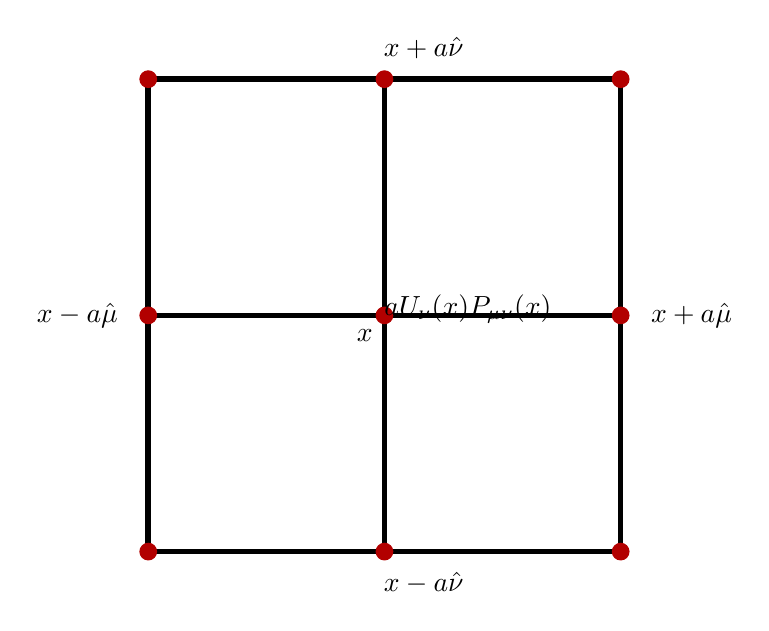
\begin{tikzpicture}
\tkzDefPoint(0,0){A}
\tkzDefPoint(3,0){B}
\tkzDefPoint(0,3){C}
\tkzDefPoint(3,3){D}

\tkzDefShiftPoint[A](0.15,-0.3){A'}
\tkzDefShiftPoint[A](-0.3,0.3){A''}
\tkzDefShiftPoint[A](0.3,0.3){A'''}
\tkzDefShiftPoint[B](-0.15,-0.3){B'}
\tkzDefShiftPoint[B](-0.3,0.3){B''}
\tkzDefShiftPoint[C](-0.3,-0.3){C'}
\tkzDefShiftPoint[C](0.3,-0.3){C''}
\tkzDefShiftPoint[D](-0.3,-0.3){D'}

\begin{scope}[very thick,decoration={
    markings,
    mark=at position 0.55 with {\arrow[scale=2.5]{stealth}}}
    ] 
\tkzDrawSegments[postaction={decorate}](A,C);
\end{scope}

\draw [step=3cm, line width=2pt] (-3-0.0001,-3-0.0001) grid (3,3);
\draw plot[mark=*,mark size = 3pt,mark options={color=black!30!red}] coordinates {(-3,-3)(0,-3)(0,0)(-3,0)(-3,3)(0,3)(3,3)(3,0)(3,-3)};
\node at (-0.25,-0.25) {$x$};
\node at (3.9,0) {$x+a\hat{\mu}$};
\node at (-3.9,0) {$x-a\hat{\mu}$};
\node at (0.5,3.4) {$x+a\hat{\nu}$};
\node at (0.5,-3.4) {$x-a\hat{\nu}$};

\begin{scope}[very thick,decoration={
    markings,
    mark=at position 0.55 with {\arrow[scale=2]{stealth}}}
    ] 
\tkzDrawSegments[postaction={decorate}](A''',B'');
\tkzDrawSegments[postaction={decorate}](B'',D');
\tkzDrawSegments[postaction={decorate}](D',C'');
\tkzDrawSegments[postaction={decorate}](C'',A''');
\end{scope}

\tkzDrawSegments[thick, <->, >=stealth](A',B') 

\tkzLabelSegment[below=-0.25,fill=white,inner sep=5pt](A',B'){$a$}
\tkzLabelSegment[left=0.15,fill=white,inner sep=5pt](A,C){$U_\nu(x)$}
\tkzLabelSegment[above=0.75](A''',B''){$P_{\mu\nu}(x)$}
\end{tikzpicture}
\caption[An example of a 2D lattice with lattice spacing $a$.]{\label{fig:LatticeExample} An example of a 2D lattice with lattice spacing $a$. From site $x$ we define $x+a\hat{\mu}$ to refer to the next lattice site in the $\hat{\mu}$ direction. The gauge links $U_\mu(x)$ (see Eq.~\eqref{eq:GaugeLink}) are defined on the links between sites. The plaquette $P_{\mu\nu}(x)$ (see Eq.~\eqref{eq:Plaquette}) is the product of the four gauge links around a $1\times 1$ loop.}
\end{figure}
%

When spacetime is discretised, it becomes necessary to consider derivatives as finite differences and integrals as finite sums.
\begin{align*}
\partial_\mu\,f(x)&\rightarrow \frac{f(x+a\hat{\mu})-f(x)}{a}\\
\int d^4x~f(x) &\rightarrow a^4\sum_x \,f(x)
\end{align*}
For example, we can construct the lattice form of Eq.~\eqref{eq:FieldStrengthTensor} as
%
\begin{equation}
F_{\text{Lat}}^{\mu\nu}(x) = \frac{A_\nu(x+a\hat{\mu})-A_\nu(x)}{a}-\frac{A_\mu(x+a\hat{\nu})-A_\mu(x)}{a}+ig[A_\mu(x),\,A_\nu(x)].
\label{eq:DiscreteFST}
\end{equation}
%
The notation $A_\nu(x+a\hat{\mu})$ denotes the field $A_\nu$ located at the site one lattice spacing in the $\hat{\mu}$ direction from $x$. We could continue to reformulate our lattice theory by imposing this method of discretisation, and indeed this is historically how the lattice framework was constructed~\cite{Wilson:1974sk}. However, it is useful to instead formulate our lattice theory in terms of gauge {\it links}. Analogous to how we introduced the covariant derivative to compensate for the fact that the quark field at infinitesimally different points in space has a different underlying gauge, we now want to have a mechanism for comparing gluon fields at some finite separation. This requires us to solve the parallel transport equation of our gauge field~\cite{Bing:1999ee,peskin2018introduction}
%
\begin{equation}
\frac{dx^\mu(t)}{dt}\,D_\mu \,U(x(t),y)=0\, ,
\label{eq:ParallelTransport}
\end{equation}
%
where $U(x(t),y)$ is an $SU(3)$ element and $x(t)$ is some path parametrised by $t\,\in\,[0,1]$ satisfying $x(0)=y$. We further require that $U(x(0),y)=I$, as the parallel transport for a fixed point is trivial. We can now make use of the explicit parametrisation of the path between two adjacent lattice sites, $x^\mu(t) = y^\mu+a\,t\,\delta_\nu^\mu$, where $y^\mu$ is a fixed position and $\nu$ is the direction we are transporting the field. It must be stressed that $\nu$ is not a free index, and thus need not be conserved on both sides of an expression. Substituting this parametrisation into Eq.~\eqref{eq:ParallelTransport} we have
\begin{align*}
&a\, \delta_\nu^\mu\, (\partial_\mu + igA_\mu)\,U(x(t),y)=0\\
&a\, \partial_\nu\, U(x(t),y) = -iag\, A_\nu\,U(x(t),y)\\
&\frac{\partial}{\partial t}\, U(x(t),y) = -iag\,A_\nu\, U(x(t),y)\, .
\end{align*}
For a non-Abelian field, this is precisely the differential equation solved by the path-ordered exponential, known as the Wilson line
%
\begin{align*}
U(x(t),y) &= \mathcal{P}\exp\left(-\int_0^t \,dt^\prime\, iag \,A_\nu(t^\prime)\right)\\
&=\mathcal{P}\exp\left(-ig\int_{y}^{y+at\hat{\nu}}\,dx^\prime\, A_\nu\left(x^\prime\right)\right)\, .
\end{align*}
%
Hence, for each direction $\hat{\mu}$, we define the gauge links between adjacent lattice sites to be
%
\begin{equation}
U_\mu(x) = \mathcal{P}\exp\left(-ig\int_x^{x+a\hat{\mu}}dx'\,A_\mu(x')\right)\, .
\label{eq:GaugeLink}
\end{equation}
%
From this definition we also see that we can write the gauge link in the opposite direction, i.e. from $x+a\hat{\mu}$ to $x$, as
%
\begin{align*}
\mathcal{P}\exp\left(-ig\int^x_{x+a\hat{\mu}}dx'\,A_\mu(x')\right) &= \mathcal{P}\exp\left(+ig\int_x^{x+a\hat{\mu}}dx'\,A_\mu(x')\right)\\
&=U^\dag_\mu(x)\, .
\end{align*}
%
These gauge links have the simple gauge transformation property~\cite{Lepage:1998dt} (see Appendix~\ref{app:WilsonLineGT})
%
\begin{equation}
U_\mu(x)\rightarrow \Omega(x)\,U_\mu(x)\,\Omega^\dag(x+a\hat{\mu})\, .
\label{eq:LinkTransformation}
\end{equation}
%
Making use of this gauge transformation property, we can construct gauge invariant Wilson loops by taking the trace of the product of the $U_\mu$'s around a closed loop. These Wilson loops form an essential building block of the lattice action, and  appear in later chapters as quantity of interest in their own right. The simplest such loop, the $1\times 1$ square, is called the \textit{plaquette}, and is defined as
\begin{equation}
P_{\mu\nu}(x) = U_\mu(x)\,U_\nu(x+a\hat{\mu})\, U_\mu^\dag(x+a\hat{\nu})\, U_\nu^\dag(x)\, .
\label{eq:Plaquette}
\end{equation}
Calculating the Wilson loop by taking the trace of the plaquette we see that by the cyclic property of the trace the Wilson loop is gauge invariant
\begin{align*}
\Tr\left(P_{\mu\nu}(x)\right)\rightarrow& \Tr \left(\Omega(x)\,U_\mu(x)\Omega^\dag(x+a\hat{\mu})\,\Omega(x+a\hat{\mu})\,U_\nu(x+a\hat{\mu})\,\Omega^\dag(x+a\hat{\mu}+a\hat{\nu})\right.\\
&~~~~~\left.\Omega(x+a\hat{\mu}+a\hat{\nu})\,U_\mu^\dag(x+a\hat{\nu})\,\Omega^\dag(x+a\hat{\nu})\,\Omega(x+a\hat{\mu})\, U_\nu^\dag(x)\,\Omega^\dag(x)\right)\\
=&\Tr\left(P_{\mu\nu}(x)\right)\, .
\end{align*}
Both the gauge links and the plaquette are also visualised in Fig.~\ref{fig:LatticeExample}.\\

We now return to the lattice formulation of QCD, making use of the gauge links to define our quantities of interest. Firstly, we approximate our gauge links on the lattice by using a midpoint definition, such that
\begin{equation}
U_\mu^\text{lat}(x) = \exp\left(-iag\, A_\mu\left(x+\frac{a}{2}\hat{\mu}\right)\right)\, .
\label{eq:GaugeLinkLat}
\end{equation}
From this definition, we can also recover the midpoint gauge potential~\cite{Leinweber:1998im,Alles:1996ka}
\begin{equation}
A_\mu\left(x+\frac{a}{2}\hat{\mu}\right) = \frac{i}{2ag}\left(U_\mu(x) - U_\mu^\dag(x)\right) - \frac{i}{6ag}\Tr\left(U_\mu(x) - U_\mu^\dag(x)\right)I + \mathcal{O}(a^2)\, .
\label{eq:GaugePotentialLat}
\end{equation}
We then note that we can write $F_{\mu\nu}$ in terms of the plaquette by Taylor expanding Eq.~\eqref{eq:Plaquette} (see Appendix \ref{app:TEPlaquette}) to obtain~\cite{Gupta:1997nd}
%
\begin{equation}
P_{\mu\nu} = I-ia^2g\, F_{\mu\nu} - \frac{a^4 g^2}{2}F^2_{\mu\nu} +\mathcal{O}(a^6)\, ,
\label{eq:PlaquetteExpansion}
\end{equation} 
%
and hence to $\mathcal{O}(a^2)$
%
\begin{align}
\frac{1}{2}\Tr\left(F_{\mu\nu}F^{\mu\nu}\right) = \sum_{\mu,\,\nu}\frac{1}{g^2}\Tr\left(I-\frac{1}{2}\left(P_{\mu\nu}+P_{\mu\nu}^\dag\right)\right)\, .
\label{eq:FieldStrengthPlaquette}
\end{align}
%
We have now arrived at a definition of the contracted field strength tensor that can be used to define our lattice action. We can make a further simplification by noting that because $P_{\mu\nu}=P_{\nu\mu}^\dagger$, $\Re(P_{\mu\nu}) = \Re(P_{\nu\mu})$ and therefore we only need to sum over the 6 plaquettes for which $\mu<\nu$, so long as we introduce a factor of $2$. This gives us the definition of the Wilson action, 
%
\begin{equation}
\mathcal{S}_\text{W} = \beta\sum_x\,\sum_{\mu<\nu} \frac{1}{3}\Tr\left(I-\frac{1}{2}\left(P_{\mu\nu}+P_{\mu\nu}^\dag\right)\right)\, ,
\label{eq:WilsonAction}
\end{equation}
%
where $\beta = \frac{6}{g^2}$ is the lattice coupling constant. To remove higher order errors from the lattice action, it is possible to take into account terms containing larger Wilson loops, following procedure similar to the one outlined above~\cite{Alford:1995hw,Symanzik:1983dc,Symanzik:1983gh}.\\

For the purpose of this work, the gauge fields were generated using the $\mathcal{O}(a^2)$-improved L\"uscher-Weisz action~\cite{Luscher:1984xn}, 
%
\begin{align}
\begin{aligned} \mathcal{S} _ { LW } = &\sum_x \left[ \frac { 5 \beta } { 9 } \sum _ { \mu < \nu } \operatorname { Tr } \left\{ 1 - \frac { 1 } { 2 } \left( P _ { \mu \nu } + P _ { \mu \nu } ^ { \dagger } \right) \right\}\right. \\
& \left.- \frac { \beta } { 36 u _ { 0 } ^ { 2 } } \sum _ { \text { rect } } \operatorname { Tr } \left\{ 1 - \frac { 1 } { 2 } \left( R _ { \mu \nu } + R _ { \mu \nu } ^ { \dagger } \right) \right\}\right]\, , \end{aligned}
\end{align}
%
where
\begin{equation}
u_0 = \left(\frac{1}{3}\operatorname{ Re } \Tr\langle P_{\mu\nu} \rangle\right)^{\frac{1}{4}}\, ,
\end{equation}
and $R_{\mu\nu}$ is the $2\times 1$ rectangle Wilson loop, defined similarly to the plaquette 
\begin{align}
\begin{array} { r l } { R _ { \mu \nu } ( x ) = } & { U _ { \mu } ( x ) U _ { \nu } ( x + \hat { \mu } ) U _ { \nu } ( x + \hat { \nu } + \hat { \mu } ) U _ { \mu } ^ { \dagger } ( x + 2 \hat { \nu } ) } \\ { } & { \times U _ { \nu } ^ { \dagger } ( x + \hat { \nu } ) U _ { \nu } ^ { \dagger } ( x ) + U _ { \mu } ( x ) U _ { \mu } ( x + \hat { \mu } ) } \\ { } & { \times U _ { \nu } ( x + 2 \hat { \mu } ) U _ { \mu } ^ { \dagger } ( x + \hat { \mu } + \hat { \nu } ) U _ { \mu } ^ { \dagger } ( x + \hat { \nu } ) U _ { \nu } ^ { \dagger } ( x ) }\, . \end{array}
\end{align}
The presence of the `tadpole' improvement factor $u_0$ is necessary to modify the coupling constant such that the action has better agreement with the continuum over small distances~\cite{Lepage:1992xa}. This choice of action provides reduced errors in comparison to the Wilson action.\\

This lattice framework provides the tools necessary to explicitly calculate quantities of interest from a first-principles standpoint. Firstly, the gauge links are generated by Monte Carlo methods, using $\exp\left(-\mathcal{S}\right)$ as a probability weighting for a given configuration. Once these configurations are generated, gauge fixing can be performed (Sec.~\ref{sec:LandauGauge}, \ref{sec:MCG}), and quantities of interest such as the gluon propagator (Chapter~\ref{chapter:GluonPropagator}) can be obtained.

\section{Gauge Fixing}
The choice of gauge is crucial when performing calculations on the lattice, or, more generally, in any gauge field theory calculation. This is because many quantities are gauge dependent, or are much simpler to calculate in a particular gauge. There are two choices of gauge relevant to this study: Landau gauge and maximal centre gauge. Maximal centre gauge is best explored in the context of centre vortices, and will therefore be detailed in chapter~\ref{sec:MCG}, however the Landau gauge fixing condition provides a good introduction to the gauge fixing procedure, and as such will be described here.

\subsection{Landau Gauge}\label{sec:LandauGauge}

In the continuum, Landau gauge corresponds to imposing the condition
\begin{equation}
\partial_\mu A^\mu = 0\, .
\label{eq:LandauGaugeCont}
\end{equation}
%
On the lattice, we can approximate this condition by imposing
\begin{equation}
\Delta(x) = \sum _ { \mu } A _ { \mu } \left( x + \frac{a}{2}\hat { \mu } \right) - A _ { \mu } \left( x-\frac{a}{2}\hat { \mu } \right) = 0\, .
\label{eq:LandauGaugeLat}
\end{equation}
Here the fact that we have defined the lattice gauge potential to be at the midpoint of the link produces an improved continuum limit when we consider Eq.~\eqref{eq:LandauGaugeLat} in momentum space~\cite{Alles:1996ka}. Performing a discrete Fourier transform, we see that
%
\begin{align}
\Delta(p) &= \sum_x \Delta(x) e^{-i\,p\cdot x} \nonumber\\
&=\sum_{x,\,\mu} e^{-i\,p\cdot x} \left(A _ { \mu } \left( x + \frac{a}{2}\hat { \mu } \right) - A _ { \mu } \left( x-\frac{a}{2}\hat { \mu } \right)\right) \nonumber\\
&= \sum_{x,\,\mu} e^{i\,p\cdot\frac{a}{2}\hat{\mu} }\,e^{-i\,p\cdot\left(x+\frac{a}{2}\hat{\mu} \right)}A _ { \mu } \left( x + \frac{a}{2}\hat { \mu } \right) - e^{-i\,p\cdot\frac{a}{2}\hat{\mu} }\,e^{-i\,p\cdot\left(x-\frac{a}{2}\hat{\mu} \right)}A _ { \mu } \left( x - \frac{a}{2}\hat { \mu } \right) \nonumber\\
&= \sum_\mu \left(e^{i\,p\cdot\frac{a}{2}\hat{\mu} } - e^{-i\,p\cdot\frac{a}{2}\hat{\mu} }\right) A_\mu(p) \nonumber\\
&=\sum_\mu 2i\sin\left(\frac{a}{2} p_\mu\right)A_\mu(p) = 0\, .
\label{eq:LandauGaugeLatP}
\end{align}
%
This is to be compared to the momentum space Landau gauge condition which can be obtained from the gauge potential defined on the lattice sites, rather than at the midpoint. If the midpoint definition is not used, the Landau gauge condition has the form~\cite{Alles:1996ka}
%
\begin{equation}
\sum _ { \mu } \left[ \left( \cos (a\,p _ { \mu }) - 1 \right) - i \sin (ap _ { \mu }) \right] A _ { \mu } ^ { \prime } ( p ) = 0\, .
\label{eq:LandauGaugeLatBad}
\end{equation}
%
In the limit as $a\rightarrow 0$, it can be seen that Eq.~\eqref{eq:LandauGaugeLatP} exhibits
$\mathcal{O}(a^2)$ improvement, whereas Eq.~\eqref{eq:LandauGaugeLatBad} has only $\mathcal{O}(a)$ improvement.\\

The Landau Gauge condition is imposed on the lattice by finding extrema of the functional~\cite{Bonnet:1999mj}
%
\begin{equation}
\mathcal{F} =  \frac{4}{3}\mathcal{F}_1 - \frac{1}{12u_0}\mathcal{F}_2\, ,
\label{eq:LGFunctional}
\end{equation}
%
where
%
\begin{align*}
\mathcal{F}_1 &= \sum _ { \mu , x } \frac { 1 } { 2 } \operatorname { Tr } \left\{ U _ { \mu } ^ { \Omega } ( x ) + U _ { \mu } ^ { \Omega } ( x ) ^ { \dagger } \right\}\\
\mathcal{F}_2 &= \sum _ { \mu , x } \frac { 1 } { 2 } \operatorname { Tr } \left\{ U _ { \mu } ^ { \Omega } ( x ) \,U _ { \mu } ^ { \Omega } ( x + a\hat { \mu } ) + U _ { \mu } ^ { \Omega } ( x + a\hat { \mu } )^\dagger\, U _ { \mu } ^ { \Omega } ( x )^\dagger  \right\}\, .
\end{align*}
%
We explicitly write $U^\Omega_\mu$ to emphasise that we are considering gauge links under an as yet unknown gauge transformation $\Omega$. It becomes apparent why we seek the extrema of this particular functional when we take the functional derivative with respect to the free parameters of the gauge transformation , $\omega^a(x)$ (see Eq.~\eqref{eq:LocalGaugeTransformation}).
%
\begin{equation}
\frac { \delta \left\{ \frac { 4 } { 3 } \mathcal { F } _ { 1 } - \frac { 1 } { 12 u _ { 0 } } \mathcal { F } _ { 2 } \right\} } { \delta \omega ^ { a } ( x ) } = g a ^ { 2 } \sum _ { \mu } \operatorname { Tr } \left\{ \left[ \partial _ { \mu } A _ { \mu } ( x ) - \frac { 4 } { 360 } a ^ { 4 } \partial _ { \mu } ^ { 5 } A _ { \mu } ( x ) + \mathcal { O } \left( a ^ { 6 } \right) \right] \frac{\lambda^a}{2} \right\} + \mathcal { O } \left( g ^ { 3 } a ^ { 4 } \right)\, .
\label{eq:LGFunctionalDeriv}
\end{equation}
%
If Eq.~\eqref{eq:LGFunctionalDeriv} is at an extrema, then 
%
\begin{equation*}
\sum_\mu \partial_\mu A_\mu(x) = \sum_\mu \frac{4}{360}a^4 \partial_\mu^5\,A_\mu(x) + \mathcal{O}(a^6)+\mathcal{O}(g^3a^4)\, .
\end{equation*}
%
Hence at order $\mathcal{O}(a^4)$, finding the extrema of Eq.~\eqref{eq:LGFunctionalDeriv} is equivalent to satisfying the continuum Landau gauge condition given in Eq.~\eqref{eq:LandauGaugeCont}. This Landau gauge fixing method gives an example of how a gauge choice can be implemented on a discrete lattice such that it approximates the continuum condition. This in turn enables us to use the continuum Landau gauge definition of the gluon propagator as described in Chapter~\ref{chapter:GluonPropagator}, which forms a vital component of this research.

\section{Lattice Units}

In the previous sections we have explicitly detailed how a variety of lattice quantities are constructed. For clarity, it is useful to remove extraneous constants by utilising so-called `lattice units'. Transforming to lattice units is done by multiplying physical quantities by relevant factors of the lattice spacing $a$ to obtain a dimensionless quantity. Some examples of lattice units are
%
\begin{align*}
x_\text{lat} &= a^{-1}\,x_\text{phys}\\
p_\text{lat} &= a\, p_\text{phys}\\
A(x)_\text{lat} &= a\, A(x)_\text{phys}\, .
\end{align*}
%
Furthermore, it is also conventional to remove factors of $g$ by setting $g=1$. These conventions have the effect of removing factors of $a$ and $g$, such that
%
\begin{align*}
A_\mu \left( x+\frac{a}{2}\hat{\mu} \right)&\rightarrow A_\mu \left(x+\frac{\hat{\mu}}{2} \right)\\
U_\mu(x) &\rightarrow \exp\left( -i A_\mu \left(x+\frac{\hat{\mu}}{2}\right)\right)\\
P_{\mu\nu}(x) &\rightarrow U_\mu(x)\,U_\nu(x+\hat{\mu})\, U_\mu^\dag(x+\hat{\nu})\, U_\nu^\dag(x)\, .
\end{align*}
%
These conventions will be adopted for the remainder of the thesis unless stated otherwise. 

%!TEX root = ../thesis.tex
%*******************************************************************************
%****************************** Third Chapter **********************************
%*******************************************************************************
\chapter{Topology of the Lattice}

% **************************** Define Graphics Path **************************
\ifpdf
    \graphicspath{{Chapter3/Figs/Raster/}{Chapter3/Figs/PDF/}{Chapter3/Figs/}}
\else
    \graphicspath{{Chapter3/Figs/Vector/}{Chapter3/Figs/}}
\fi
QCD presents two key properties that distinguish it from the other forces of nature:
\begin{enumerate}
\item Confinement of quarks, resulting in the absence of isolated quarks.
\item Dynamical chiral symmetry breaking, leading to dynamical generation of mass. This results in a substantial discrepancy between the mass of hadrons and the sum of the masses of the quarks that comprise them.
\end{enumerate}
These properties are experimentally verified to exist in nature, however the question of how they arise from the gauge theory of QCD developed in the preceding chapter is still the subject of intense investigation. It is believed that both these properties are connected by some underlying topological structure of the QCD vacuum. Proposed candidates include Abelian monopoles~\cite{tHooft:1981bkw,Smit:1989vg,Matsubara:1993nq,Suzuki:1989gp,Mandelstam:1974pi,Kronfeld:1987ri}, instantons~\cite{Belavin:1975fg,Witten:1978bc,Callan:1977gz,Schafer:1996wv,Trewartha:2013qga,Aharonov:1978jd} and centre vortices~\cite{'tHooft:1977hy,'tHooft:1979uj,Feynman:1981ss,Aharonov:1978jd,Cornwall:1979hz,Nielsen:1979xu}. With the advent of lattice simulations, the most promising of these appears to be the centre vortex model. Numerical evidence from the lattice has been amassed that indicates that topological objects known as centre vortices are tied to both confinement and dynamical chiral symmetry breaking~\cite{Biddle:2018dtc,Faber:1997rp,Langfeld:1998cz,Bowman:2008qd,Trewartha:2015ida,Trewartha:2015nna,Trewartha:2017ive,DelDebbio:1996lih,Greensite:2003bk,DelDebbio:1998luz,OMalley:2011aa,Langfeld:2003ev}. It is therefore the subject of this research to further extend the investigation into the properties of centre vortices, specifically in the gluonic sector of QCD.\\

As dynamical chiral symmetry breaking is primarily concerned with quarks, we will omit a detailed discussion of this property and instead begin this chapter outlining the confinement property exhibited by the strong force. We will then introduce centre vortices and motivate how they provide a potential explanation for confinement in QCD. From here we will survey the lattice results found in current literature pertaining to centre vortices, and describe how it is that we can identify centre vortices on the lattice. Finally we will briefly describe instantons and topological charge, in preparation for later chapters that draw on these concepts.  
\section{Confinement}\label{sec:Confinement}
The confinement property of QCD, and the accompanying notion of asymptotic freedom, is one of the defining low-energy features of the theory of the strong interaction. With Gell-mann and Zweig's concurrent proposal of quarks as the elementary constituents of baryons and mesons~\cite{GellMann:1964nj,Zweig:1964jf}, it is natural to then attempt to observe these new particles in isolation. However, efforts to observe quarks proved impossible. Early experiments testing the behaviour of electron-proton collisions demonstrated that protons scatter elastically, behaving as though they are finite-sized particles recoiling electromagnetically from the incident electron~\cite{Hofstadter:1956qs}. These experiments indicated no further substructure to the proton, inconsistent with the quark model. As accelerator energies improved, later experiments~\cite{Bloom:1969kc, Breidenbach:1969kd}, using electron energies of $7$ and $10~\si{GeV}$ found that inelastic scattering effects became dominant, with electrons behaving as though they were scattering off of loosely bound constituent particles. To explain this behaviour, Feynman proposed what is known as the 'parton' model~\cite{Feynman:1969ej}, treating the proton as being comprised of non-interacting electrically charged particles in the limit that the incident electron energy tends towards infinity. This is precisely the notion of asymptotic freedom; at large distance scales the partons are tightly bound, whereas at short distances they behave as free particles. It did not take long for the separate theories of quarks and partons to recognised as complementary, and by the early 70's the quark-parton model of hadrons accurately explained the the experimental results observed in particle colliders.\\

These experimental and theoretical results led in part to the development of the non-Abelian gauge field theory of QCD, as introduced in Chapter~\ref{chapter:LatticeQCD}. The proof that non-Abelian gauge theories are asymptotically free was discovered in 1973~\cite{Gross:1973id}, and experimental evidence of the existence of 3 quark colours through study of the cross section of $e^+ e^-$ collisions supports the initial $SU(3)$ colour symmetry anticipated by Gell-Mann and Zweig. At high energies, QCD has consistently explained the behaviour of hadronic matter, and has become the accepted theory of the strong nuclear interaction. However, the question of whether QCD is indeed a confining theory still remains. As confinement is a low-momentum property of QCD, it is apparent that any analytic proof of confinement must take place far from the asymptotic limit. To date, no such analytic proof has been found.\\

Lattice calculations are currently the only method by which it is possible to investigate low-energy QCD phenomena from first-principles. Calculations of the static potential between two massive quarks, both recent and old~\cite{Born:1993cq, Bonnet:1999gt, Creutz:1980hb, DiGiacomo:1990hc}, have shown that the potential rises linearly at sufficiently large separation distances. This behaviour is precisely what is expected of a colour confining theory. Other confinement mechanisms have also been proposed on the lattice, including mechanisms based on the behaviour of the gluon propagator at $q=0$~\cite{Zwanziger:1991gz} and the behaviour of the pion mass and Polyakov loop at light quark masses~\cite{Iwasaki:1991mr}. All lattice results so far have indicated that QCD is in fact a confining theory at low energy.\\

There is good evidence that confinement has its roots in the topological properties of the QCD vacuum. It is well understood that the QCD vacuum, unlike the QED vacuum, admits non-trivial instanton solutions: solutions of the vacuum field configurations that are all minima of the classical action, yet are distinguished from one another by a topological quantum number~\cite{Belavin:1975fg}. The presence of instanton solutions was significant in resolving the $U(1)$ anomaly~\cite{tHooft:1986ooh}, and provides an excellent method of calculating the ground state hadron spectrum~\cite{Schafer:1996wv}. The non-trivial topology of the QCD vacuum, and the success of topological features in resolving QCD anomalies, motivates the search for a topological explanation of confinement. A variety of features have been proposed, including: Abelian monopoles~\cite{Ivanenko:1990xu, Chernodub:1995tt}, merons~\cite{Callan:1977qs} and dual superconductors~\cite{Mandelstam:1974pi,tHooft:1982ylj}. One of the most promising models in recent years is known as the \textit{Centre Vortex Model}, and it is this model that forms the backbone of this research.

\section{Centre Vortices}
Originally proposed by 't Hooft in 1978~\cite{'tHooft:1977hy,'tHooft:1979uj}, centre vortices are closed two-dimensional surfaces present in four-dimensional Euclidean space that carry colour-magnetic flux. The key property of a centre vortex is that in three dimensions, where the vortices appear as tubes, any Wilson loop (see Sec.~\ref{sec:LatticeDiscretisation}) that encloses a vortex will acquire a centre phase, such that
%
\begin{equation}
W(C)\rightarrow z \,W(C)\, ,
\end{equation}
%
where $z$ is an element of $Z(3)$, the centre of $SU(3)$. The centre of a group is the subgroup that contains all the elements of the group that commute with all other elements. In the case of $SU(3)$ this corresponds to
%
\begin{equation}
Z(3) = \big\lbrace \exp\left(\frac{m\pi i}{3} \right)I ~ | ~ m = 0,\pm 1\big\rbrace\, . 
\end{equation}
%
When considering the value of any given Wilson loop, the centre vortex model suggests that
%
\begin{equation}
W(C) = \prod_i z_i\times \lbrace\text{short-distance physics}\rbrace\, ,
\end{equation}
%
where the $z_i$ correspond to the phases of the centre vortices intersecting the loop $C$. A simple visualisation of this idea is shown in Fig.~\ref{fig:CentreVortex}. It is not immediately apparent why this form of the Wilson loop is related to confinement, however a simple $SU(3)$ calculation motivates the relevance of this model~\cite{Greensite:2016pfc}. To understand the significance of this calculation it is worth first deviating slightly to detail the relationship between the Wilson loop and the potential energy between two massive (static) quarks.\\
% 
\begin{figure}
\centering
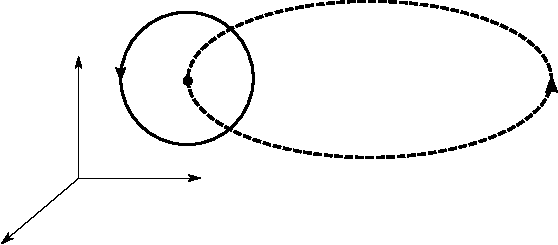
\includegraphics[width=\linewidth]{./centre_vortex.pdf}
\caption{\label{fig:CentreVortex} A single centre vortex (dashed line) intersecting a Wilson loop (solid line) in 3 dimensions. The Wilson loop will acquire a centre phase corresponding to the phase of the vortex.}
\end{figure}
%

Follwing the argument presented in Ref.~\cite{Makeenko:2009dw}, consider a Wilson loop calculated around a rectangle in the $x-t$ plane with dimensions $R\times T$. As the Wilson loop is gauge invariant, we are free to select a convenient gauge in which to perform the calculation. To this end, we choose the fields to be in axial gauge, such that $A_0(x)=0\implies U_0(x) = 1\,\forall\,x$. So the Wilson loop becomes
%
\begin{equation}
W(R\times T) = \Tr \left(U_1(0)\,U_1^\dagger(T)\right)\, .
\end{equation}
%
We can insert a complete set of energy eigenstates, $\sum_n |\,n\rangle\,\langle n \,|=1$ to obtain
%
\begin{align*}
W(R\times T) &= \Tr \left( \sum_n \langle U_1(0)\, |\, n\rangle\,\langle n\, |\, e^{-E_n(R)\, T}\, | \, U_1(0) \rangle\right)\\
&=  \sum_n \Tr \left( \big|\langle U_1(0)\, |\, n\rangle\big|^2 \right)\,e^{-E_n(R)\,T} 
\end{align*}
%
As $T\rightarrow \infty$, the only surviving contribution will be the lowest energy, $E_0(R)$. This means that
%
\begin{equation}
\lim_{T\rightarrow \infty} W(R\times T) \propto e^{-E_0(R)\, T}\, .
\label{eq:WilsonEnergy}
\end{equation}
\\

With Eq.~\ref{eq:WilsonEnergy} in mind, we return to the aforementioned $SU(3)$ confinement model. Consider a two-dimensional plane with area $L^2$, with $2N$ vortices piercing the plane. Assuming an even distribution of vortices, the total vortex density is $\rho = \frac{2N}{L^2}$. As there are two $SU(3)$ vortex types, corresponding to the two non-trivial phases $\exp\left(\frac{\pm 2\pi i}{3}\right)$, we assume that there is an equal distribution of vortex phases, i.e. there are $N$ vortices of each type. The probability of finding $n$ vortices of a given phase in some region of the plane $A\subseteq L^2$ is equal to the probability that exactly $n$ vortices are in $A$, multiplied by the probability that exactly $N-n$ vortices are outside of $A$, multiplied by the number of ways this situation can occur. Expressed mathematically, this is
%
\begin{equation}
P_N(n) = {N\choose n} \left(\frac{A}{L^2}\right)^n \left(1-\frac{A}{L^2}\right)^{N-n}\, .
\end{equation}
%
The expectation value of the Wilson loop around the perimeter of $A$ can be written as
%
\begin{equation}
\langle W(\partial A)\rangle = \sum_{m,n = 0}^N \left(\exp\left(\frac{2\pi i}{3}\right)\right)^n P_N(n)\, \left(\exp\left(\frac{2\pi i}{3}\right)\right)^m P_N(m)\, .
\end{equation}
%
If we assume the vortex phases are uncorrelated, then we can make use of the following property of uncorrelated random variables $X$ and $Y$
%
\begin{equation}
E[XY] = E[X]E[Y]\, ,
\end{equation}
%
to write
%
\begin{equation}
\langle W(\partial A)\rangle = \sum_{n=0}^N \left(\exp\left(\frac{2\pi i}{3}\right)\right)^n P_N(n)\,\sum_{m=0}^N \left(\exp\left(\frac{2\pi i}{3}\right)\right)^m P_N(m)\, .
\label{eq:WilsonExpectation}
\end{equation}
%
We consider just the first sum in Eq.~\ref{eq:WilsonExpectation} and calculate
%
\begin{align*}
\sum_{n=0}^N \left(\exp\left(\frac{2\pi i}{3}\right)\right)^n P_N(n) & = \left(1-\frac{A}{L^2}\right)^{N}\sum_{n=0}^{N} {N\choose n} \left(\exp\left(\frac{2\pi i}{3}\right)\,\frac{A}{L^2}\left(1-\frac{A}{L^2}\right)^{-1}\right)^n\\
&=\left(1+\left(\exp\left(\frac{2\pi i}{3}\right) - 1\right)\frac{A}{L^2}\right)^N\, ,
\end{align*}
%
where we have made use of the binomial series to evaluate the sum. Hence the total expectation value is
%
\begin{align}
\langle W(\partial A)\rangle &=\left(1+\left(\exp\left(\frac{2\pi i}{3}\right) - 1\right)\frac{A}{L^2}\right)^N\, \left(1+\left(\exp\left(\frac{-2\pi i}{3}\right) - 1\right)\frac{A}{L^2}\right)^N\nonumber\\
&=\left(1 -3\frac{A}{L^2} + 3\left(\frac{A}{L^2}\right)^2\right)^N\nonumber\\
&= \left(\left(\frac{A}{L^2}\right)^3+\left(1-\frac{A}{L^2}\right)^3\right)^N\, .\label{eq:WilsonExpectationSimple}
\end{align}
%
Rewriting Eq.~\ref{eq:WilsonExpectationSimple} in terms of the vortex density $\rho$, we have
%
\begin{equation}
\langle W(\partial A)\rangle = \left(\left(\frac{A\rho}{2N}\right)^3+\left(1-\frac{A\rho}{2N}\right)^3\right)^N\, .
\end{equation}
%
Now we take the limit as $N,L^2\rightarrow\infty$, keeping $\rho$ constant. Taking the limit, we find
%
\begin{equation}
\langle W(\partial A)\rangle = \exp\left(-\frac{3}{2}\rho A\right)
\label{eq:WilsonAreaLaw}
\end{equation}
%
Letting $A=R\times T$ as in Eq.~\ref{eq:WilsonEnergy}, we see that $E_0(R) = -\frac{3}{2}\rho R$, so the static quark potential rises linearly with distance between them, exactly as it should in a confining theory. Eq.~\ref{eq:WilsonAreaLaw} demonstrates an {\it area law} behaviour of the Wilson loop; this is often taken as a requirement for confinement~\cite{DelDebbio:1998luz,Dosch:1988ha}.\\

%
\begin{figure}[h]
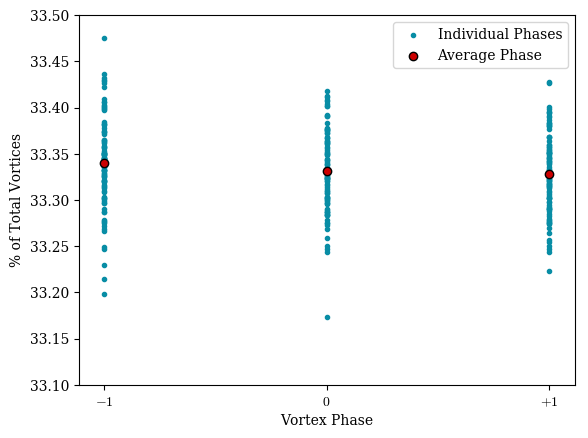
\includegraphics{./VortexDistribution.png}
\caption{\label{fig:VortexDistribution}A plot of the vortex phase distribution of 100 Monte-Carlo generated configurations, as a percentage of the total number of vortices. The method by which vortices are identified will be detailed in Sec.~\ref{sec:LocatingVortices}.}
\end{figure}
%
It is important to highlight the assumptions and simplifications made in the above argument. Most easily addressed is the assumption that there is an equal number of $+1$ and $-1$ vortices. By identifying vortices in Monte-Carlo generated configurations and plotting the distribution of phases in Fig.~\ref{fig:VortexDistribution}, we see that there is little deviation from an even distribution, especially in the ensemble average. This is an expected result, as we shall see later that vortices are required to form closed loops in 3D to conserve the vortex flux, so a vortex line should pierce a 2D surface once in each direction, corresponding to the two non-trivial phases.\\

The assumption that the vortex density is constant is, however, less well motivated. So far we have treated vortices as infinitesimally thin sheets in 4D, which is not physically motivated. An infinitely thin vortex introduces a singularity in the action, as the vortex flux must be constrained to an infinitely thin cross-section. Rather, physical vortices are `thick'; they have a finite cross-section in the direction perpendicular to the vortex sheet. If the vortex is contained entirely within the area $A$ it contributes the centre phase as described above. However, as $A$ approaches the size of the vortex cross section, one must account for vortices that are only partially inside $A$, and thus not necessarily contributing a pure centre phase. Although this consideration spoils the elegance of the above confinement mechanism for small Wilson loops, it does potentially save the model from a previously noted pitfall related to the Casimir scaling of the Wilson loop expectation value~\cite{Greensite:1982be}, as will be described in more detail in Sec.~\ref{}. Finally, it is worth noting that this issue is only relevant to Wilson loops of similar size to the vortex cross-section. As the Wilson loop increases in size, the majority of the vortices will be contained entirely within the loop, with a diminishing number of thick vortices overlapping the perimeter of the loop, as shown in Fig.~\ref{fig:VortexSizes}.\\
%
\begin{figure}[htb!]
\centering
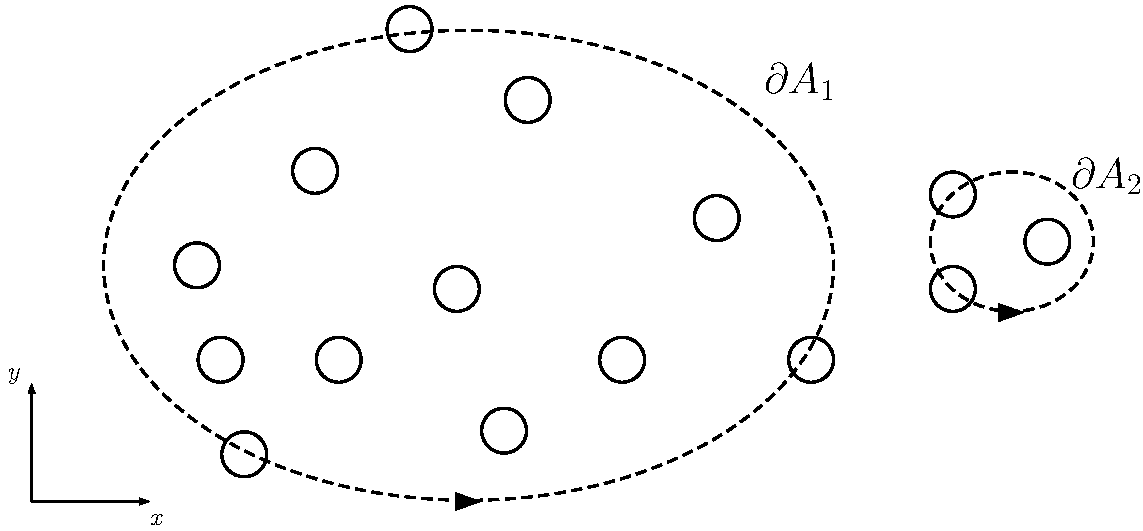
\includegraphics[width=\linewidth]{./LargeVortex.pdf}
\caption{\label{fig:VortexSizes}An example of two Wilson loops (dashed lines) lying in a plane, pierced by vortices of finite cross-section (solid lines). \textbf{Left:} The majority of vortices contributing to the phase are fully contained within the large loop, with only a few overlapping at the perimeter. \textbf{Right:} For a small loop, the contribution from overlapping vortices is significant as there are few vortices fully inside the loop.}
\end{figure}

The final assumption is that the vortex locations are random and uncorrelated from one another. This is perhaps the most significant assumption made in the above picture, as can be seen from the following calculation~\cite{Engelhardt:1999fd}. As vortices must form closed lines in 3D, let us suppose that instead of being randomly distributed, the vortices come in pairs separated by a maximum distance $d$. This corresponds to requiring that vortex lines form a closed loop of some maximum diameter $d$. If this vortex line pierces the Wilson loop in both directions, then the product of the phases, $\exp\left(\frac{2\pi i}{3}\right)\times \exp\left(\frac{-2\pi i}{3}\right) = 1$, results in no contribution to the Wilson loop. Hence, the only vortices capable of contributing a non-trivial phase to the Wilson loop are those contained within a strip of width $d$ about the perimeter of the loop. Note that not every vortex within this strip will contribute a non-trivial phase, as for example the vortex may be smaller than $d$ or oriented such that the vortex flows in direction of $\partial A$ and thus still pierces twice. We will take the most generous case, however, and assume that every vortex piercing this strip contributes a non-trivial phase. To first order, the area of relevance to to the expectation value of the Wilson loop is now $A_\text{strip}=\partial A\, d$. The probability to find $N$ vortices lying within this strip is 
%
\begin{equation}
P_N(n) = {N\choose n} \left(\frac{\partial A d}{L^2}\right)^n \left(1-\frac{\partial A d}{L^2}\right)^{N-n}\, .
\end{equation}
%
By following the same steps used to arrive at Eq.~\ref{eq:WilsonAreaLaw}, we find
%
\begin{equation}
\langle W(\partial A)\rangle = e^{-\frac{3}{2}\rho\, d\, \partial A}\, .
\end{equation}
%
So we see that instead of an area law, we now have a perimeter law for the Wilson loop, dependent on the upper bound for the vortex size. This implies that if there is some upper limit on the size of a vortex, we can no longer expect to see confining behaviour. We deduce therefore that to obtain a confining theory, it is necessary to allow the vortex size to be potentially infinite. In the language of the vortex model, this is called \textit{vortex percolation}. Conversely, the presence of an upper bound on the vortex size would imply a deconfined phase. This suggests that the size of vortices can be used as an \textit{order parameter} for confinement~\cite{Langfeld:1998cz}, with two distinct phases:
\begin{enumerate}
\item Vortex percolation $\implies$ confinement.
\item Loss of vortex percolation $\implies$ deconfinement.
\end{enumerate}
\subsection{Current Evidence for Centre Vortices}
\subsubsection{String Tension}

\subsubsection{Hadron Spectrum}

\subsubsection{Mass Function}

\subsubsection{Gluon Propagator}

\subsubsection{Casimir Scaling}


\section{Locating Centre Vortices}\label{sec:LocatingVortices}
\subsection{Maximal Centre Gauge}\label{sec:MCG}
\subsection{Centre Projection}
\section{Further Topological Quantities}
\subsection{Instantons}
\subsection{Topological Charge}

%A frequently seen mistake is to use `\textbackslash begin\{center\}' \dots `\textbackslash end\{center\}' inside a figure or table environment. This center environment can cause additional vertical space. If you want to avoid that just use `\textbackslash centering'
%
%
%\begin{table}
%\caption{A badly formatted table}
%\centering
%\label{table:bad_table}
%\begin{tabular}{|l|c|c|c|c|}
%\hline 
%& \multicolumn{2}{c}{Species I} & \multicolumn{2}{c|}{Species II} \\ 
%\hline
%Dental measurement  & mean & SD  & mean & SD  \\ \hline 
%\hline
%I1MD & 6.23 & 0.91 & 5.2  & 0.7  \\
%\hline 
%I1LL & 7.48 & 0.56 & 8.7  & 0.71 \\
%\hline 
%I2MD & 3.99 & 0.63 & 4.22 & 0.54 \\
%\hline 
%I2LL & 6.81 & 0.02 & 6.66 & 0.01 \\
%\hline 
%CMD & 13.47 & 0.09 & 10.55 & 0.05 \\
%\hline 
%CBL & 11.88 & 0.05 & 13.11 & 0.04\\ 
%\hline 
%\end{tabular}
%\end{table}
%
%\begin{table}
%\caption{A nice looking table}
%\centering
%\label{table:nice_table}
%\begin{tabular}{l c c c c}
%\hline 
%\multirow{2}{*}{Dental measurement} & \multicolumn{2}{c}{Species I} & \multicolumn{2}{c}{Species II} \\ 
%\cline{2-5}
%  & mean & SD  & mean & SD  \\ 
%\hline
%I1MD & 6.23 & 0.91 & 5.2  & 0.7  \\
%
%I1LL & 7.48 & 0.56 & 8.7  & 0.71 \\
%
%I2MD & 3.99 & 0.63 & 4.22 & 0.54 \\
%
%I2LL & 6.81 & 0.02 & 6.66 & 0.01 \\
%
%CMD & 13.47 & 0.09 & 10.55 & 0.05 \\
%
%CBL & 11.88 & 0.05 & 13.11 & 0.04\\ 
%\hline 
%\end{tabular}
%\end{table}
%
%
%\begin{table}
%\caption{Even better looking table using booktabs}
%\centering
%\label{table:good_table}
%\begin{tabular}{l c c c c}
%\toprule
%\multirow{2}{*}{Dental measurement} & \multicolumn{2}{c}{Species I} & \multicolumn{2}{c}{Species II} \\ 
%\cmidrule{2-5}
%  & mean & SD  & mean & SD  \\ 
%\midrule
%I1MD & 6.23 & 0.91 & 5.2  & 0.7  \\
%
%I1LL & 7.48 & 0.56 & 8.7  & 0.71 \\
%
%I2MD & 3.99 & 0.63 & 4.22 & 0.54 \\
%
%I2LL & 6.81 & 0.02 & 6.66 & 0.01 \\
%
%CMD & 13.47 & 0.09 & 10.55 & 0.05 \\
%
%CBL & 11.88 & 0.05 & 13.11 & 0.04\\ 
%\bottomrule
%\end{tabular}
%\end{table}

%!TEX root = ../thesis.tex
%*******************************************************************************
%*********************************** Fourth Chapter *****************************
%*******************************************************************************

\chapter{Lattice Configurations and the Gluon Propagator}\label{chapter:GluonPropagator}
\ifpdf
    \graphicspath{{Chapter4/Figs/Raster/}{Chapter4/Figs/PDF/}{Chapter4/Figs/}}
\else
    \graphicspath{{Chapter4/Figs/Vector/}{Chapter4/Figs/}}
\fi

Now that we have developed the required background understanding of lattice QCD and the topological objects of interest to this research, we can detail how our calculations are performed. This chapter will first describe how we calculate the primary quantity of interest, the Landau gauge gluon propagator, on the lattice. We will then motivate our choice of momentum variables, before proceeding to a description of the lattice parameters and data cuts utilised in this work.

\section{Lattice Definition of the Gluon Propagator}
In a gauge field theory the position-space propagator, $D_{\mu\nu}(x,y)$, of the gauge boson is the two-point correlation function. In the case of QCD this can be interpreted as the probability amplitude of a gluon being created at the space-time point $x$, propagating to $y$, and then being annihilated. The propagator therefore serves as a useful measure of the behaviour of gluons as a function of distance; or, correspondingly, as a function of momentum in the momentum-space representation. In this section we detail how the Landau gauge gluon propagator is calculated on the lattice. We begin with the definition of the coordinate space propagator as a two-point correlator~\cite{Zwanziger:1991gz,Cucchieri:1999sz,Langfeld:2001cz}.
\begin{equation}
D^{ab}_{\mu\nu}(x) = \langle A^a_\mu(x) \, A^b_\nu(0)\rangle.
\label{eq:coordGluonProp}
\end{equation}
The propagator in momentum space is simply related by the discrete Fourier transform,
\begin{equation}
D^{ab}_{\mu\nu}(p) = \sum_x e^{-ip\cdot x} \langle A^a_\mu(x) \, A^b_\nu(0) \rangle. 
\end{equation}
Noting that the coordinate space propagator $D^{ab}_{\mu\nu}(x-y)$ only depends on the difference $x-y,$ such that
\begin{equation}
\langle A^a_\mu(x) \, A^b_\nu(0)\rangle = \langle A^a_\mu(x+y) \, A^b_\nu(y)\rangle\, ,
\end{equation}
we can make use of translational invariance to average over the four-dimensional volume to obtain the form for the momentum space propagator.
\begin{align}
D^{ab}_{\mu\nu}(p) &= \frac{1}{V}\sum_{x,y} e^{-ip\cdot x}\langle A^a_\mu(x+y) \, A^b_\nu(y) \rangle \nonumber \\
                &= \frac{1}{V}\sum_{x,y} \langle e^{-ip\cdot (x+y)} A^a_\mu(x+y) \, e^{+ip\cdot y}A^b_\nu(y) \rangle \nonumber \\
                &= \frac{1}{V}\langle A^a_\mu(p) \, A^b_\nu(-p) \rangle. \label{eq:gluPropxtop}
\end{align}

Hence we find that the momentum space gluon propagator on a finite lattice with four-dimensional volume $V$ is given by
%
\begin{equation}
D_{\mu\nu}^{ab}(p) \equiv \frac{1}{V}\left \langle A^a_\mu (p)\,A^b_\nu(-p)\right\rangle \, . \label{eq:gluonProp}
\end{equation}
%
In the continuum, the Landau-gauge momentum-space gluon propagator has the following form~\cite{Leinweber:1998im,Bonnet:2001uh}
%
\begin{equation}
D^{ab}_{\mu\nu}(p) = \left ( \delta_{\mu\nu} - \frac{p_\mu p_\nu}{p^2} \right )\,\delta^{ab}\,D(p^2) \, ,
\end{equation}
%
where $D(p^2)$ is the scalar gluon propagator.  Contracting Gell-Mann index $b$ with $a$ and
Lorentz index $\nu$ with $\mu$ one has
%
\begin{equation}
D^{aa}_{\mu\mu}(p) = (4-1)\,(n_c^2-1)\,D(p^2) \, ,
\end{equation}
%
such that the scalar function can be obtained from the gluon propagator via
%
\begin{equation}
D(p^2) = \frac{1}{3(n_c^2-1)}\,D^{aa}_{\mu\mu}(p) \, ,
\label{eq:scalarProp}
\end{equation}
%
where $n_c = 3$ is the number of colours.

As the lattice gauge links $U_\mu(x)$ naturally reside in the $3\times 3$ fundamental representation of $SU(3),$ we now wish to work in the matrix representation of $A_\mu(x)$, as introduced in Eq.~\ref{eq:CovariantDerivative}. Using the orthogonality relation $\Tr(\lambda_a\lambda_b) = 2\delta_{ab}$ for the Gell-Mann matrices, it is straightforward to see that
%
\begin{equation}
2\Tr(A_\mu\,A_\mu) = A^a_\mu A^a_\mu\, ,
\end{equation}
%
which can be substituted into equation~\ref{eq:scalarProp} to obtain the final expression for the lattice scalar gluon propagator,
%
\begin{equation}
D(p^2) = \frac{2}{3\,(n_c^2-1)\,V}\big\langle {\rm Tr}\, A_\mu(p)\,A_\mu(-p) \big\rangle \,. \label{eq:scalarProp2}
\end{equation}

To calculate Eq.~\ref{eq:scalarProp2} on the lattice, we need to define $A_\mu(p)$. As defined in Eq.~\ref{eq:GaugePotentialLat}, we make use of the midpoint definition of the coordinate-space gauge potential in terms of the lattice link variables. Once the link variables are fixed to Landau gauge following the procedure described in Sec.~\ref{sec:LandauGauge}, we can obtain the momentum-space gauge potential by performing a Fourier transform,
%
\begin{equation}
A_\mu(p) = \sum_x e^{-ip\cdot(x+\hat{\mu}/2)}\, A_\mu(x+\hat{\mu}/2)\, .
\end{equation}
%
We have now constructed the necessary tools to calculate the Landau gauge scalar gluon propagator within the lattice framework established in Chapter \ref{chapter:LatticeQCD}.

\section{Momentum Variables}\label{sec:MomentumVariables}
As discussed in Sec.~\ref{sec:Confinement}, it is understood that at QCD is asymptotically free. With this understanding, we expect that at high momentum the Landau gauge gluon propagator will tend towards the Landau gauge photon propagator~\cite{ryder1996quantum}
%
\begin{equation}
D_\gamma(p^2) = \frac{1}{p^2}\, .
\end{equation}
%
However, lattice discretisation errors cause a deviation from this idealised behaviour that we would like to systematically account for. To do this, we follow the work of Refs.~\cite{Weisz:1982zw, Weisz:1983bn,Luscher:1985zq,Symanzik:1983dc,Symanzik:1983gh} and consider the behaviour of the photon propagator on the lattice. We therefore consider for this section only an Abelian theory. The field strength tensor is then simplified to
%
\begin{equation}
F_{\mu\nu} = \partial_\mu \,A_\nu - \partial_\nu\,A_\mu
\end{equation}
%
We consider this Abelian field to be on a lattice generated using the Wilson action (see Eq.~\ref{eq:WilsonAction}). From Eq.~\ref{eq:FieldStrengthPlaquette} we know that the Wilson action can be written as $\mathcal{S}_\text{W} = a^4\frac{1}{2}\sum_x F_{\mu\nu}F^{\mu\nu} + \mathcal{O}(a^4)$. As we are interested in the momentum-space propagator, we write the field strength tensor at the plaquette midpoint $\tilde{x}$ as
%
\begin{align*}
F_{\mu\nu}(\tilde{x}) &= \sum_p e^{ip\tilde{x}} \left(\frac{A_\nu\left(\tilde{x}+a\frac{\hat{\mu}}{2}\right) - A_\nu\left(\tilde{x}-a\frac{\hat{\mu}}{2} \right)}{a} - \frac{A_\mu\left(\tilde{x}+a\frac{\hat{\nu}}{2}\right) - A_\mu\left(\tilde{x}-a\frac{\hat{\nu}}{2} \right)}{a}\right)\\
&= \frac{1}{a} \sum_p e^{ip\tilde{x}} \left(\tilde{A}_\nu(p)\, e^{-iap\frac{\hat{\mu}}{2}} - \tilde{A}_\nu(p)\, e^{iap\frac{\hat{\mu}}{2}} - \tilde{A}_\mu(p)\, e^{-iap\frac{\hat{\nu}}{2}} + \tilde{A}_\mu(p)\, e^{iap\frac{\hat{\nu}}{2}}\right)\\
&= -\frac{1}{a} \sum_p e^{ip\tilde{x}}\left(2i\sin\left(\frac{a p_\mu}{2}\right)\tilde{A}_\nu(p) - 2i\sin\left(\frac{a p_\nu}{2}\right)\tilde{A}_\mu(p)\right)\\
&= - \sum_p e^{ip\tilde{x}}\tilde{f}_{\mu\nu}(p)\, ,
\end{align*}
%
where
%
\begin{equation}
\tilde{f}_{\mu\nu}(p) = i\left(\hat{k}_\mu \tilde{A}_\nu(p) - \hat{k}_\nu \tilde{A}_\mu(p)\right)\, ,~\hat{k}_\mu = \frac{2}{a}\sin\left(\frac{ap_\mu}{2}\right)\, .
\end{equation}
%
The Wilson action can therefore be written as
%
\begin{align}
\mathcal{S}_\text{W} &= a^4\frac{1}{2}\sum_{\tilde{x}}\sum_{p,\,p^\prime}e^{i\tilde{x}(p+p^\prime)}\tilde{f}_{\mu\nu}(p) \, \tilde{f}^{\mu\nu}(p^\prime)\nonumber\\
&=a^4\frac{1}{2}\sum_{p,\,p^\prime} \delta(p+p^\prime)\tilde{f}_{\mu\nu}(p) \, \tilde{f}^{\mu\nu}(p^\prime) \nonumber\\
&= a^4\frac{1}{2}\sum_{p}\tilde{f}_{\mu\nu}(p) \, \tilde{f}^{\mu\nu}(-p) + \mathcal{O}(a^4)\, . \label{eq:WilsonMomentum}
\end{align}
%
We are now in a position to consider the propagator. Equivalent to the two-point correlator definition, the propagator is also the Green's function of the equations of motion, satisfying
%
\begin{equation}
M_{\mu\nu}D^{\nu\lambda}(p) = \delta_\mu^\lambda\, .
\end{equation}
%
In the continuum, we can write the Abelian Lagrangian in terms of momentum space variables as 
%
\begin{align*}
\mathcal{L} &= \frac{1}{2}\tilde{F}_{\mu\nu}\,\tilde{F}^{\mu\nu}\\
&= \frac{1}{2}(k_\mu\,\tilde{A}_\nu - k_\nu\,\tilde{A}_\mu)\,(k^\mu\,\tilde{A}^\nu - k^\nu\,\tilde{A}^\mu)\\
&= (k^2\delta_{\mu\nu} - k_\mu\,k_\nu)\tilde{A}^\mu\,\tilde{A}^\nu\, ,
\end{align*}
%
and hence
%
\begin{equation}
M_{\mu\nu} = (k^2\delta_{\mu\nu} - k_\mu\,k_\nu)\, .
\label{eq:ContEquationsOfMotion}
\end{equation}
%
However, it is understood that in the continuum the equations of motion are not invertible unless an additional gauge fixing term is added, with a gauge fixing parameter $\alpha$. Hence, the equations of motion for the photon field in momentum space are given by Eq.~\ref{eq:ContEquationsOfMotion} with an additional gauge fixing term~\cite{ryder1996quantum}
%
\begin{equation}
M_{\mu\nu} = k^2\delta_{\mu\nu} - \left(1-\frac{1}{\alpha}\right)k_\mu k_\nu\, .
\end{equation}
%
By inspection, we see that Eq.~\ref{eq:WilsonMomentum} will have the same equations of motion, with the substitution $k_\mu\rightarrow \hat{k}_\mu$. In turn, this gives the propagator
%
\begin{equation}
D_{\mu\nu}(p) = \frac{1}{\hat{k}^2}\left[\delta_{\mu\nu} + (\alpha-1)\frac{\hat{k}_\mu \hat{k}_\nu}{\hat{k}^2}\right]\, .
\end{equation}
Landau gauge corresponds to setting $\alpha=0$, so we find that
%
\begin{equation}
D_{\mu\mu}(p) = \frac{3}{\hat{k}^2}\, ,
\end{equation}
%
and therefore by comparison with Eq.~\ref{eq:scalarProp} we see that
%
\begin{equation}
D(p^2) = \frac{1}{\hat{k}^2}\, .
\end{equation}
%
This suggests that for the Wilson action we should make the substitution $p_\mu\rightarrow q_\mu = \hat{k}_\mu = \frac{2}{a}\sin\left(\frac{a p_\mu}{2}\right)$ so that at tree-level we observe the expected behaviour of the gluon propagator.\\

A similar analysis can be performed for the L\"uscher and Weisz action, taking into account the contributions from the rectangle terms. The L\"uscher and Weisz action written in the same form as Eq.~\ref{eq:WilsonMomentum} is~\cite{Weisz:1982zw}
%
\begin{equation}
\mathcal{L}_\text{LW} = a^4\frac{1}{2}\sum_p \left(1+\frac{1}{12}a^2\hat{k}^2\right) \tilde{f}_{\mu\nu}(p) \, \tilde{f}^{\mu\nu}(-p) + \mathcal{O}(a^6)\, .
\end{equation}
%
The equations of motion then become
%
\begin{equation}
M_{\mu\nu} = \left(\hat{k}^2 + \frac{1}{12}a^2\hat{k}^4\right)\delta_{\mu\nu} - \left(1-\frac{1}{\alpha}\right)\left(\sqrt{\hat{k}_\mu^2 + \frac{1}{12}a^2\hat{k}_\mu^4}\right)\left(\sqrt{\hat{k}_\nu^2 + \frac{1}{12}a^2\hat{k}_\nu^4}\right)\, .
\end{equation}
Therefore the propagator is
%
\begin{equation}
D_{\mu\nu}(p) = \frac{1}{\hat{q}^2}\left[\delta_{\mu\nu} + (\alpha-1)\frac{\hat{q}_\mu \hat{q}_\nu}{\hat{q}^2}\right]\, ,
\end{equation}
with
\begin{equation}
q_\mu = \sqrt{\hat{k}_\mu^2 + \frac{1}{12}a^2\hat{k}_\mu^4} = \frac{2}{a}\sqrt { \sin ^ { 2 } \left( \frac { p _ { \mu } a } { 2 } \right) + \frac { 1 } { 3 } \sin ^ { 4 } \left( \frac { p _ { \mu } a } { 2 } \right) }\, .
\end{equation}
%
In Landau gauge, this suggests the tree-level form for the scalar propagator is
%
\begin{equation}
D(p^2) = \frac{a^2}{4 \sin ^ { 2 } \left( \frac { p _ { \mu } a } { 2 } \right) + \frac { 1 } { 3 } \sin ^ { 4 } \left( \frac { p _ { \mu } a } { 2 } \right)} = \frac{1}{q^2}\, .
\label{eq:LWCorrection}
\end{equation}\\

For this work, we make the variable substitution $p_\mu\rightarrow q_\mu$ to ensure that at high momentum where we expect the gluon propagator to tend towards tree level we observe that $q^2 D(q^2) = 1$. The momentum variables chosen for both the Wilson and L\"uscher and Weisz action have been numerically verified to provide better tree level agreement in Refs.~\cite{Marenzoni:1994ap, Bonnet:2001uh}, and we present a comparison of the L\"uscher and Weisz and uncorrected variables in Fig.~\ref{fig:MomentumComparison}. We plot $k^2\,D(k^2)$ (where $k_\mu$ is the momentum variable for the given case under consideration) such that the tree-level propagator appears as $k^2\,D(k^2)=1$, shown as the black dashed line. We can clearly see that at high momenta the corrected gluon propagator tends towards the expected tree-level behaviour, whereas the uncorrected propagator fans out considerably. This fanning is the result of asymmetry between the spacial and temporal components of the propagator, which is accounted for in the tree-level correction~\cite{Marenzoni:1994ap}. The results presented in Fig.~\ref{fig:MomentumComparison} clearly motivate the need for tree-level correction when calculating the gluon propagator on the lattice.\\
%
\begin{figure}[htb!]
\centering
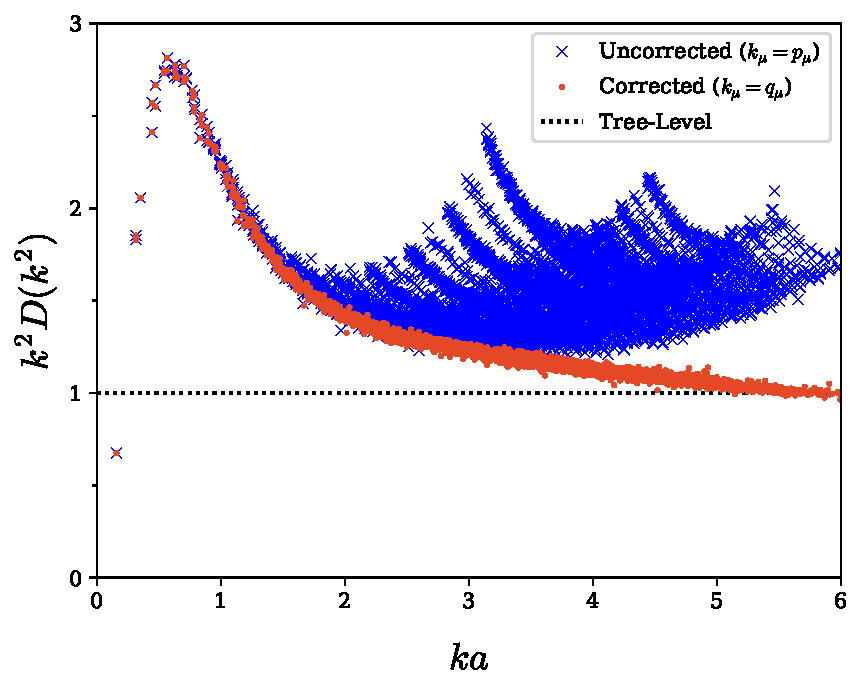
\includegraphics[width=\linewidth]{./ScalarGluComp_q2_MomentumComparison.pdf}
\caption{\label{fig:MomentumComparison} The scalar gluon propagator is plotted with no tree-level momentum correction (blue crosses) and the L\"uscher and Weisz correction (red dots) presented in Eq.~\ref{eq:LWCorrection}. It is clear that the corrected momentum has improved tree-level behaviour, free from the fanning effect present in the uncorrected case.}
\end{figure}
%
\section{Lattice Parameters and Data Cuts} \label{sec:LatticeParameters}
We calculate the gluon propagator on 100 configurations of a $20^3\times 40$ $SU(3)$ lattice with spacing $a=0.125\,\si{fm}$, as used in Refs.~\cite{Trewartha:2015nna,OMalley:2011aa}. When considering the gluon propagator it is useful to maintain the plotting convention introduced in Fig.~\ref{fig:MomentumComparison} of considering $q^2D(q^2)$ against $qa$. This has the twofold benefit of both aiding in visualisation of the tree-level behaviour, and enabling clearer analysis of the infrared properties of the propagator by suppressing the low-$qa$ region. Following the procedure of Ref.~\cite{Bonnet:2001uh,Leinweber:1998im} all results are plotted after a momentum half-cut. The momentum half-cut corresponds to only considering lattice momenta in the range
%
\begin{equation}
p_\mu = \frac{2\pi n_\mu}{a N_\mu},~n_\mu\in \left(-\frac{N_\mu}{4},\,\frac{N_\mu}{4}\right]\, .
\end{equation}
%
This cut limits the positive range of the kinematically corrected $q_\mu$ to
%
\begin{equation}
q_\mu \in \left[0,\, \frac{2\sqrt{21}}{3a}\right]\approx\left[0,3.06\right]\, .
\end{equation}
%
Furthermore, a cylinder cut of radius $pa=2$ lattice units is performed such that we only consider points within two lattice units of the diagonal. This cut is implemented by considering points satisfying
%
\begin{equation}
|pa|^2\, \sin(\theta_c) \leq 2\, ,
\end{equation}
%
where
%
\begin{equation}
\theta_c = \cos^{-1}\left(\frac{pa \cdot \hat{n}}{|pa|}\right)\, ,
\end{equation}
%
and $\hat{n} = \frac{1}{2}(1,\,1,\,1,\,1)$ is the unit vector along the diagonal. This is performed so that all directions are equally sampled, whilst omitting points where one direction dominates the signal. This assists in filtering out high-momentum systematic errors. Finally, we can take advantage of the rotational symmetry of the scalar propagator to perform $Z(3)$ averaging over the Cartesian coordinates. This means that we average over all points with the same Cartesian radius; for example, we would average across the points $(n_x,n_y,n_z)=(2,1,1),\,(1,2,1)$ and $(1,1,2)$. These choices of cuts assist in producing a cleaner signal that accurately represents the behaviour of the continuum propagator.\\

With these cuts implemented, the gluon propagator on the untouched configurations appears as Fig.~\ref{fig:UntouchedPropagator}. We observe the expected tree-level behaviour at high momenta, with an infrared enhancement indicative of amplified low-momentum propagation. Due to the cuts we have made, we observe a much cleaner signal, particularly in the region $qa\geq 1.5$, in agreement with the results of Ref.~\cite{Bonnet:2001uh}. It should be noted that the difference in peak height observed between Fig.~\ref{fig:MomentumComparison} and Fig.~\ref{fig:UntouchedPropagator} is due to a different renormalisation constant. This issue will be discussed in detail in Sec.~\ref{sec:Renormalisation}.
%
\begin{figure}[htb!]
\centering
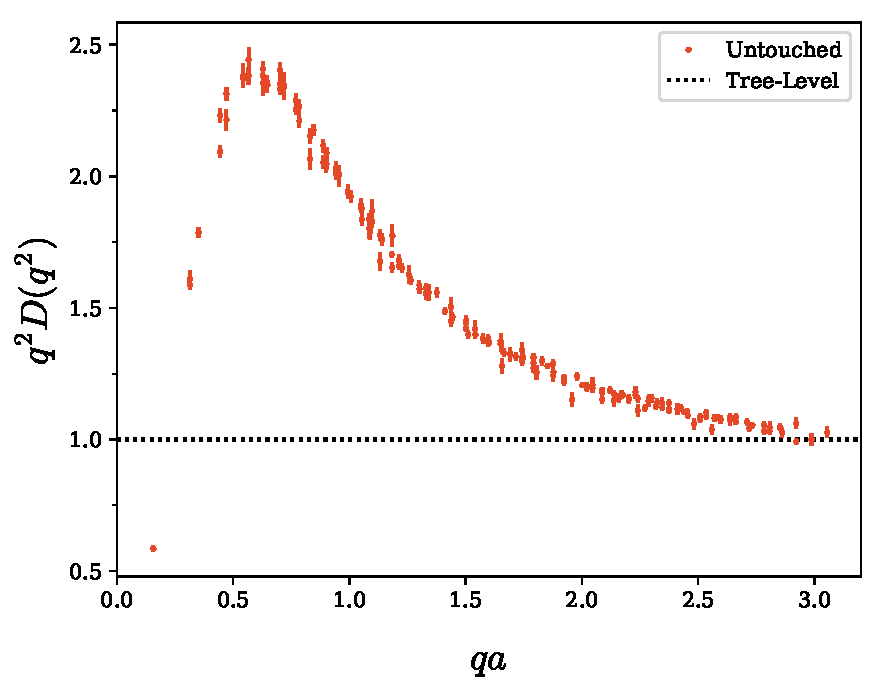
\includegraphics[width=\linewidth]{./ScalarGluComp_q2_NoCoolU.pdf}
\caption{\label{fig:UntouchedPropagator} The untouched gluon propagator with all data cuts and correct momentum variables utilised. We observe a substantially cleaner signal when compared to the untouched propagator shown in Fig.~\ref{fig:MomentumComparison}.}
\end{figure}



%!TEX root = ../thesis.tex
%*******************************************************************************
%*********************************** Fifth Chapter *****************************
%*******************************************************************************

\chapter{Smoothing}\label{chapter:Smoothing}
\ifpdf
    \graphicspath{{Chapter5/Figs/Raster/}{Chapter5/Figs/PDF/}{Chapter5/Figs/}}
\else
    \graphicspath{{Chapter5/Figs/Vector/}{Chapter5/Figs/}}
\fi

Lattice definitions of topological objects are plagued by random fluctuations originating from the Monte-Carlo generation of lattice configurations and as a result identification of topological objects can give inaccurate or even nonsensical results. Hence, when considering the behaviour of topological objects on the lattice, it has been proven to be necessary to remove the high frequency fluctuations in the gauge fields~\cite{Bonnet:2000dc}. Furthermore, when investigating the long range behaviour of the lattice it is also beneficial to filter off the short distance fluctuations to better reveal the physics in the domain of interest~\cite{Moran:2008ra}. This filtering process is known as smoothing, and it forms an important step in any study of lattice topological objects and long range behaviour. For example, it has previously been shown that smoothing is necessary to obtain agreement between the untouched and vortex only string tension, mass function and instanton content~\cite{Trewartha:2015ida,Trewartha:2015nna,Trewartha:2017ive}. The process of smoothing in turn falls into two sub-categories: cooling and smearing.\\

The purpose of both these methods is similar, however, the algorithms used to implement them differ. Cooling assesses each link in turn, replacing the existing link with one that locally minimises some choice of action (see e.g. the Wilson action, Eq.~\ref{eq:WilsonAction}). Rather than explicitly minimising a given action, smearing  instead replaces each link with a weighted average of its nearest neighbours. Once every link in the lattice has been updated according to one of these methods, the configuration is said to have had one sweep of smoothing applied. The process can then be repeated to an arbitrary number of sweeps to achieve the desired degree of smoothness.  Due to the differences in the routines, it is important to compare the results from both to observe how they each perform and quantify how they alter the result.

\section{Smoothing Methods}
\subsection{Cooling}
Cooling is the original method devised for smoothing lattice gauge fields, first utilised in an analysis of the topological susceptibility of simplified lattice models~\cite{Berg:1981nw}. It was shown early on that the process of cooling can be used to distinguish between `genuine' topological charge that is representative of classical minima of the action, and background Monte-Carlo topological charge brought about by random fluctuations created during the generation of the lattice configuration. Under cooling, the former is preserved whilst the latter is annihilated. The process of cooling according to the simplest Wilson action is based on the method outlined by Cabibbo and Marinari~\cite{Cabibbo:1982zn,Creutz:1980zw}, and is performed as follows.\\

We first define the `staple' associated with a link $U_\mu$. A staple is the product of all the link variables around a chosen loop, except for the link being cooled. For example, the $1\times 1$ plaquette staple associated with $U_\mu$ is
%
\begin{equation}
\tilde { U }^{1\times 1} _ { \mu \nu}(x) = U _ { \nu } ( x + \hat { \mu } ) U _ { \mu } ^ { \dagger } ( x + \hat { \nu } ) U _ { \nu } ^ { \dagger } ( x )\, .
\end{equation}
%
Graphically, this can be seen as in Fig.~\ref{fig:Staple}. Larger staples are defined similarly; for example a $2\times 2$ staple corresponds to the product of seven of the eight links in the $2\times 2$ square, with $U_\mu(x)$ omitted. For the Wilson action, which is all we shall consider for now, the six unique $1\times 1$ staples are the only ones required. Once all relevant staples are calculated, they are summed to obtain
%
\begin{equation}
\bar{U} = \sum_{\alpha = 1} ^ 6 \tilde{U}_\alpha\, ,
\label{eq:Staples}
\end{equation}
where $\alpha$ enumerates the staples, not the Lorentz index. We can now rewrite the Wilson action associated with a single link $U_\mu$ as, 
%
\begin{equation}
S(U_\mu) = 3 - \operatorname{Re}\Tr (U_\mu \bar{U})\, ,
\label{eq:WilsonActionCool}
\end{equation}
%
which is a different, but completely equivalent, form of Eq.~\ref{eq:WilsonAction}.\\ % 
\begin{figure}[ht!]
\centering
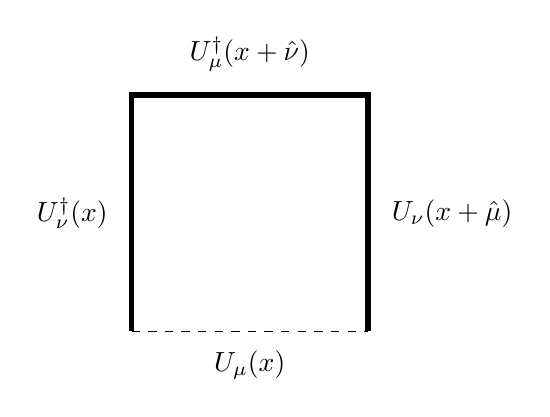
\begin{tikzpicture}
\draw[line width = 2pt] (0,-3) -- (0,0)node[midway, label=right:{$U_\nu(x+\hat{\mu})$}]{} -- (-3,0)node[midway, label=above:{$U_\mu^\dag(x+\hat{\nu})$}]{} -- (-3,-3)node[midway, label=left:{$U_\nu^\dag(x)$}]{};
\draw[dashed] (-3,-3) -- (0,-3)node[midway, label=below:{$U_\mu(x)$}]{};
%\draw plot[mark=*,mark size = 3pt,mark options={color=red}] coordinates {(-3,-3)(0,-3)(0,0)(-3,0)};
\end{tikzpicture}
\caption[An example $1\times 1$ staple.]{\label{fig:Staple} An example $1\times 1$ staple, with the dashed link indicating the link the staple is relative to. The origin of the name staple is apparent from the shape of the 3 solid links.}
\end{figure}
%

The objective of cooling is to select a new $SU(3)$ matrix, $U_\mu^\prime$, to replace $U_\mu$ with such that $U_\mu^\prime$ minimises Eq.~\ref{eq:WilsonActionCool}. This is equivalent to maximising
%
\begin{equation}
R = \operatorname{Re} \Tr (U_\mu^\prime \, \bar{U})\, .
\label{eq:CoolFunctional}
\end{equation}
%
Naively, it would seem that $U_\mu^\prime = \bar{U}^{-1}$ would be the ideal choice. However, $\bar{U}$ is a sum of $SU(3)$ matrices, and $SU(3)$ is only closed under multiplication, not addition. Hence, $\bar{U}$, and by extension $\bar{U}^{-1}$, are not necessarily in $SU(3)$, making $\bar{U}^{-1}$ and invalid substitute for $U_\mu$. However, any $SU(2)$ element can be written in the form $U = a _ { 0 } I + i \vec { a } \cdot \vec { \sigma }$, where $\vec{\sigma}$ are the Pauli matrices and $a\in\mathbb{R}^4$  satisfies $a^2=1$. Hence, a sum of $SU(2)$ elements will be proportional to another $SU(2)$ element. We can exploit this fact to construct an new $SU(3)$ element from three $SU(2)$ subgroups. To this end, we wish to find a $U^\prime$ of the form
%
\begin{equation}
U^\prime_\mu = a_3\,a_2\,a_1\,U_\mu\, ,
\label{eq:UPrime}
\end{equation}
%
where the $a_i$ are each in different a $3\times 3$ representation of $SU(2)$. The optimal choice is
%
\begin{align*}
a_1 &= \frac{1}{k_1}
\begin{pmatrix}
\frac{1}{2}\left((U_\mu \, \bar{U})_{11} + (U_\mu \, \bar{U})^*_{22}\right) & \frac{1}{2}\left((U_\mu \, \bar{U})_{12} - (U_\mu \, \bar{U})^*_{21}\right) & 0\\
\frac{1}{2}\left((U_\mu \, \bar{U})_{21} - (U_\mu \, \bar{U})^*_{12}\right) & \frac{1}{2}\left((U_\mu \, \bar{U})^*_{11} + (U_\mu \, \bar{U})_{22}\right) & 0\\
0 & 0 & k_1
\end{pmatrix}^\dagger\\
a_2 &= \frac{1}{k_2}
\begin{pmatrix}
\frac{1}{2}\left((U_\mu \, \bar{U})_{22} + (U_\mu \, \bar{U})^*_{33}\right) & 0 & \frac{1}{2}\left((U_\mu \, \bar{U})_{23} - (U_\mu \, \bar{U})^*_{32}\right)\\
0 & k_2 & 0\\
\frac{1}{2}\left((U_\mu \, \bar{U})_{32} - (U_\mu \, \bar{U})^*_{23}\right) & 0 & \frac{1}{2}\left((U_\mu \, \bar{U})^*_{22} + (U_\mu \, \bar{U})_{33}\right)
\end{pmatrix}^\dagger\\
a_3 &= \frac{1}{k_3}
\begin{pmatrix}
0 & 0 & k_3\\
0 & \frac{1}{2}\left((U_\mu \, \bar{U})_{11} + (U_\mu \, \bar{U})^*_{33}\right) & \frac{1}{2}\left((U_\mu \, \bar{U})_{13} - (U_\mu \, \bar{U})^*_{31}\right)\\
0 & \frac{1}{2}\left((U_\mu \, \bar{U})_{31} - (U_\mu \, \bar{U})^*_{13}\right) & \frac{1}{2}\left((U_\mu \, \bar{U})^*_{11} + (U_\mu \, \bar{U})_{33}\right)
\end{pmatrix}^\dagger\, .
\end{align*}
The factor of $\frac{1}{k_i}$ fixes the determinant such that $\det(a_i)=1$. The procedure for identifying these $SU(2)$ elements is described in detail in Appendix~\ref{app:Cooling}. With this construction of $U_\mu^\prime$ we locally minimise the Wilson action for each link. This determination of $U_\mu^\prime$ is repeated 12 times per link. One sweep of cooling constitutes updating each link on the lattice according to this procedure.\\

As detailed in Ref.~\cite{Bonnet:2000dc}, this process can be thought of as locally minimising the Wilson action of the three $SU(2)$ subgroups, which collectively minimises the Wilson action of the full $SU(3)$ link. It is then simple to extend this procedure to different actions by expanding the size and shape of the staples considered in the construction of $\bar{U}$. As all of the quantities utilised in the cooling procedure are gauge invariant, cooling can be performed in any gauge to arrive at the same cooled configuration. Cooling also maintains the Boltzmann distribution of the lattice links~\cite{Cabibbo:1982zn}, indicating that the new links can be considered a thermalised distribution. However, cooling is not a gauge transformation, and as such it represents a deviation from the original physical configuration. We therefore need to be careful when selecting the action used for the cooling routine to ensure that we are not removing the physics that we are interested in. To best study instantons and topological charge on a periodic lattice, it has been shown that a $\mathcal{O}(a^4)$ three-loop  improved action is most suitable~\cite{BilsonThompson:2002jk}. This action is dubbed a `three-loop' action as it consists of a linear combination of $1\times 1$, $2\times 2$ and $3\times 3$ Wilson loops. This choice of action combines both computational efficiency with an effective stabilisation of instantons and an accurate preservation of the topological charge under repeated cooling sweeps. As a result, it is this three-loop cooling routine that will be utilised in this research.

\subsection{Over-Improved Smearing}
Despite the accurate results obtained from cooled lattice configurations, cooling presents certain computational inefficiencies. Given that the staples, $\bar{U}_\alpha$ must remain constant while updating a given link $U_\mu$, there are limitations to how  parallelised the algorithm can be, especially for larger combinations of loops such as those used in the chosen three-loop improved action. To avoid these issues, a different type of smoothing was developed, known as `smearing'. Rather than locally minimising the action by direct substitution of each link, the initial APE smearing~\cite{Albanese:1987ds, Falcioni:1984ei} routine replaces each link with a weighted average of its nearest neighbours, according to
%
\begin{equation}
U^\prime = (1-\alpha)\,U_\mu + \frac{\alpha}{6}\,\bar{U}^\dagger\, ,
\end{equation}
%
where $\bar{U}$ is the sum of the staples given in Eq.~\ref{eq:Staples} and $\alpha$ is some weighting parameter. However, as stated in the previous section, a linear combination of $SU(3)$ matrices is not necessarily in $SU(3)$, so APE smearing is dependent on a choice of projection into the $SU(3)$ group. To remove the need for this projection step, the method of stout-link smearing was developed~\cite{Morningstar:2003gk}.\\

We will first outline the stout-link smearing algorithm, then extend this to the over-improved stout-link smearing employed in this research. To begin, we define
%
\begin{equation}
\Sigma_\mu = \rho_\text{sm}\,(U_\mu\,\bar{U})^\dagger\, ,
\end{equation}
%
where $\rho_\text{sm}$ is a smearing constant chosen to remain fixed for all lattice sites and $\bar{U}$ is the sum of the relevant staples depending on the choice of action. Using this definition we construct
%
\begin{equation}
Q_\mu = \frac{i}{2}\left( \Sigma_\mu^\dagger - \Sigma_\mu \right) - \frac{i}{6}\Tr\left(\Sigma_\mu^\dagger - \Sigma_\mu\right)I\, .
\end{equation}
By construction, $Q_\mu$ is Hermitian ($Q_\mu = Q_\mu^\dagger$) and traceless, so it belongs to the $SU(3)$ Lie algebra. It can therefore be exponentiated to obtain an element of $SU(3)$. We then define the new smeared link by
%
\begin{equation}
U_\mu^\prime = \exp(iQ_\mu)\,U_\mu\, .
\end{equation}
%
This definition effectively corresponds to a complex sum of neighbouring link combinations, however it has numerically been demonstrated to give similar results to the previous APE smearing technique, provided that the smearing parameter $\rho_\text{sm}$ is selected appropriately~\cite{Morningstar:2003gk}. For this work, we choose $\rho_\text{sm}=0.06$, in accordance with the results of Ref.~\cite{Moran:2008ra}. As in the case of cooling, the choice of staples used to define $\bar{U}$ has significant impact on the behaviour of topological objects under smearing. To this end, work has been done to tune the smearing algorithm so that it preserves instanton-like objects under repeated smearing sweeps, leading to the development of over-improved stoutlink smearing~\cite{Moran:2008ra}.\\

To see the necessity for over-improved stoutlink smearing, it is important to detail how we quantitatively measure the effect of smearing on topological objects. To do this, we calculate the instanton action in terms of the instanton radius. The error terms in the instanton action then give an indication of how the instanton radius will change as the action decreases under smearing. This in turn gives an indication of how well the smearing routine preserves topological objects. If the Baker-Campbell-Hausdorff plaquette expansion given in Appendix~\ref{app:TEPlaquette} is instead truncated at $\mathcal{O}(a^4)$ rather than $\mathcal{O}(a^2)$, the Wilson action becomes~\cite{GarciaPerez:1993lic}
%
\begin{equation}
\mathcal{S}_\text{W} = a^4\sum_x\,\sum_{\mu,\,\nu} \Tr\left[\frac{1}{2}F_{\mu\nu}^2 + \frac{a^2}{24}\left\lbrace \left( D _ { \mu } F _ { \mu \nu } ( x ) \right) ^ { 2 } + \left( D _ { \nu } F _ { \mu \nu } ( x ) \right) ^ { 2 } \right\rbrace + \mathcal{O}(a^4)\right]\, .
\end{equation}
%
Substituting in the instanton potential (Eq.~\ref{eq:InstantonSolution}) and field strength tensor (Eq.~\ref{eq:InstantonFieldStrength}), we find that the Wilson action goes like
%
\begin{equation}
S_\text{W}^\text{inst} = \frac{8\pi^2}{g^2}\left\{1-\frac{1}{5}\left(\frac{a}{\rho}\right)^2 + \mathcal{O}\left(\frac{a}{\rho}\right)^4 \right\}\, ,
\end{equation}
%
where $\rho$ is the instanton radius. We note then that as the Wilson action is minimised, the $-\frac{1}{5}\left(\frac{a}{\rho}\right)^2$ term must become increasingly negative, implying that the instanton radius decreases. This is precisely the effect we wish to avoid, as the instanton radius will shrink under smearing to the point where the instanton-like objects `fall through' the lattice as $\rho\rightarrow a$. A similar calculation can be done for the L\"uscher and Weisz action, showing that~\cite{GarciaPerez:1993lic}\\
%
\begin{equation}
S_\text{LW}^\text{inst} = \frac{8\pi^2}{g^2}\left\{ 1 - \frac { 17 } { 210 } \left(  \frac{a}{\rho} \right) ^ { 4 } + \mathcal { O } \left( \frac{a}{\rho} \right) ^ { 6 } \right\}\, .
\end{equation}
%

In both of the previous instanton actions, the leading error term is negative, resulting in a suppression of the instanton radius. To counteract this we `over-improve' the action by modifying it to be a linear combination of $S_\text{W}$ and $S_\text{LW}$, introducing a parameter $\epsilon$ that interpolates between them~\cite{Moran:2008ra}. This modified action is given as
%
\begin{equation}
S ( \epsilon ) =  \beta \sum _ { x } \sum _ { \mu > \nu } \left[ \frac { 5 - 2 \epsilon } { 3 } \left( 1 - P _ { \mu \nu } ( x ) \right) - \frac { 1 - \epsilon } { 12 } \left( \left( 1 - R _ { \mu \nu } ( x ) \right) + \left( 1 - R _ { \nu \mu } ( x ) \right) \right) \right]\, .
\end{equation}
%
We see that $S(1)=S_\text{W}$ and $S(0) = S_\text{LW}$. Expanding $S(\epsilon)$ in terms of the instanton solution, we have
%
\begin{equation}
S^\text{inst}(\epsilon) = \frac { 8 \pi ^ { 2 } } { g ^ { 2 } } \left[ 1 - \frac { \epsilon } { 5 } \left( \frac { a } { \rho  } \right) ^ { 2 } + \frac { 14 \epsilon - 17 } { 210 } \left( \frac { a } { \rho } \right) ^ { 4 } + \mathcal { O } \left( \frac{a}{\rho} \right) ^ { 6 } \right]\, .
\end{equation}
%
The parameter $\epsilon$ can now be tuned so as to preserve instantons under smearing. Performing stoutlink smearing with this choice of action dependent on $\epsilon$ is known as over-improved stoutlink smearing. When using this routine, it is necessary to select appropriate $\rho_{\text{sm}}$ and $\epsilon$ parameters. We keep the previous value of $\rho_{\text{sm}}=0.06$, however there is some subtlety to finding an appropriate $\epsilon$. The natural choice for $\epsilon$ may be to follow Ref.~\cite{GarciaPerez:1993lic} and set $\epsilon=-1$ to ensure that the leading error term is positive. However, one then runs the risk of unphysically growing the instanton size such that it annihilates with anti-instantons present on the lattice. Furthermore, we wish to smear such that the instantons are minimally distorted as they undergo the smearing process. To this end, we follow the results of Ref.~\cite{Moran:2008ra} and choose $\epsilon = -0.25$. We then choose the corresponding staple parameter $\bar{U}$ to be the sum over the $1\times 1$ and $(2\times 1) + (1\times 2)$ loops with $U_\mu$ omitted, with respective weightings $\frac{5-2\epsilon}{3}$ and $-\frac{1-\epsilon}{12}$. We can now utilise this over-improved stoutlink smearing routine to filter out short distance physics, isolating the topological objects of interest.

\section{Results from the Gluon Propagator}\label{sec:CoolingGluProp}

Making use of the smoothing methods defined above, we now wish to compare their effect on the gluon propagator. Summarising the previous sections, we employ $\mathcal{O}(a^4)$-improved three-loop cooling and over-improved stoutlink smearing with smearing parameters $\rho_\text{sm}=0.06$ and $\epsilon=-0.25$. We first plot the untouched propagator after 0, 1, 2, 4 and 8 sweeps of cooling in Fig.~\ref{fig:1to10SweepsCooling}. In gauge fixing to Landau gauge, each sweep has been preconditioned by the Landau gauge transformation of the prior sweep in descending order (i.e. the transformation for sweep 10 preconditions sweep 9). This preconditioning is done to ensure that the Landau gauge functional is near the same local minima for each cooling sweep. We observe the expected removal of short distance fluctuations that is typical of smoothing, resulting in a suppressed propagator at large $q$. This is complemented by an amplification in the infra-red region which can be attributed to the increase in low momentum modes arising from the smoothing of the gauge fields.\\
%
\begin{figure}[tb]
\centering
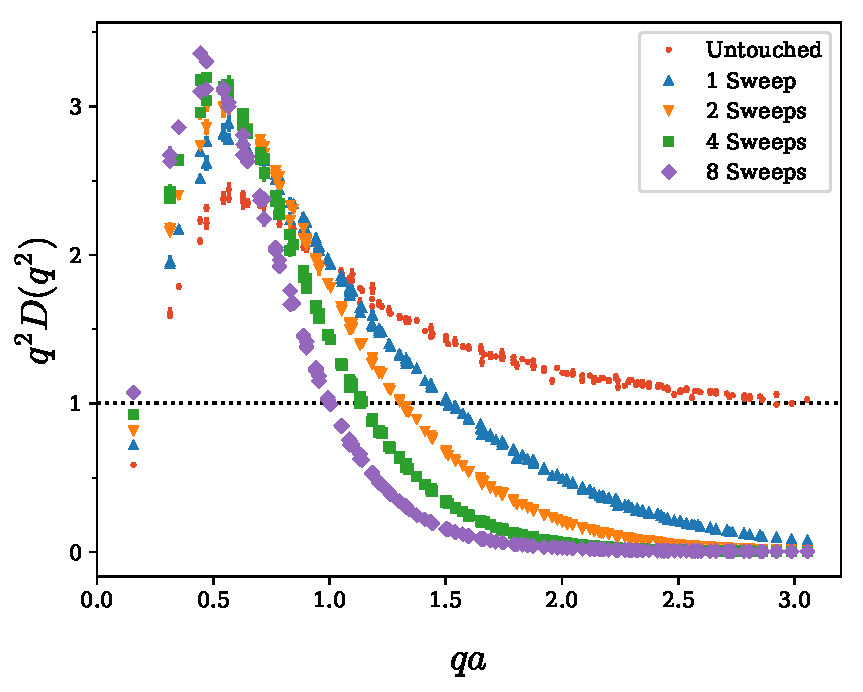
\includegraphics[width=\linewidth]{./ScalarGluComp_q2_1to10sweeps.pdf}
\caption[Comparison of the gluon propagator on the untouched configurations after cooling.]{\label{fig:1to10SweepsCooling}Comparison of the gluon propagator on the untouched configurations after cooling. For clarity we have selected a sample of sweeps between 1 and 8.}
\end{figure}
%

To compare the effects of cooling and over-improved smearing, the untouched gluon propagator is plotted in Fig.~\ref{fig:SmearCoolComp} after either over-improved smearing or cooling. By comparing the smeared and cooled propagator we can see that cooling has a more rapid effect, related to the well-known fast removal of action from the lattice. The qualitative shape of the propagator remains the same however, and it can be seen that, for example, 4 smearing sweeps produces a propagator remarkably similar to 1 cooling sweep. More generally, we observe that in regards to the shape of the propagator, $n_{\text{sm}}\approx4\,n_{\text{cool}}$. Following the observation made in Ref.~\cite{Thomas:2014tda} that the number of over-improved stoutlink smearing sweeps is related to the gradient flow time by
%
\begin{equation}
t\approx\rho\,n_{\text{sm}}\, ,
\end{equation}
%
we deduce that the relationship between gradient flow time and cooling is
\begin{equation}
t\approx0.24\,n_{\text{cool}}\,.
\end{equation}\\
%
\begin{figure}[tb]
\centering
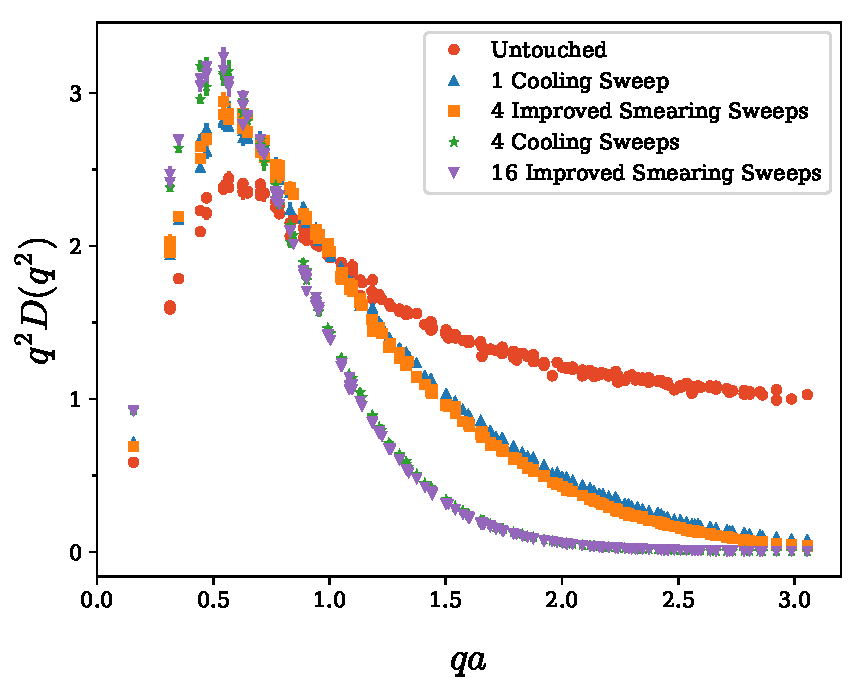
\includegraphics[width=\linewidth]{./ScalarGluComp_q2_SmearCoolComp.pdf}
\caption[The gluon propagator after cooling or improved smearing.]{\label{fig:SmearCoolComp}The gluon propagator after cooling or improved smearing. We see that the shape of the plot changes minimally between the smoothing routines. However cooling requires fewer sweeps to produce the same effect when compared to smearing.}
\end{figure}
%

It is well understood that smoothing alters the vortex background, and based on previous work~\cite{Cais:2008za,Trewartha:2015ida,DelDebbio:1998luz} we anticipate that the vortices identified on smoothed configurations would differ to those identified on the unsmoothed configurations. We therefore perform vortex identification only on the untouched configurations, with smoothing then being performed independently on the untouched, vortex-only and vortex-removed configurations, as shown in Chapter~\ref{chapter:GluonPropagatorResults}. We choose to use cooling as the smoothing algorithm for the results presented in this research as it lowers the action of the lattice configurations faster than over-improved smearing, however it is worth noting that similar results can be obtained with the use of over-improved smearing. With this understanding of smoothing routines developed, we are now in a position to calculate the gluon propagator on our vortex modified configurations. We are now free to employ cooling to filter out the long-range physics and isolate the vortex contribution to the propagator, illuminating the significance of centre vortices. 


%!TEX root = ../thesis.tex
%*******************************************************************************
%*********************************** Sixth Chapter *****************************
%*******************************************************************************

\chapter{Gluon Propagator on Vortex-Modified Backgrounds}
\ifpdf
    \graphicspath{{Chapter6/Figs/Raster/}{Chapter6/Figs/PDF/}{Chapter6/Figs/}}
\else
    \graphicspath{{Chapter6/Figs/Vector/}{Chapter6/Figs/}}
\fi
Here we present the results from the gluon propagator, calculated according to method outlined in Chapter~\ref{chapter:GluonPropagator}, on our three vortex-modified configurations:
\begin{enumerate}
\item Original `untouched' fields, $U_{\mu}(x),$

\item Projected vortex-only fields, $Z_{\mu}(x),$

\item Vortex-removed fields, $R_\mu(x) = Z^{\dagger}_{\mu}(x)\,U_{\mu}(x).$
\end{enumerate} 
\section{Preliminary Results}

\begin{figure}[tb]
\centering
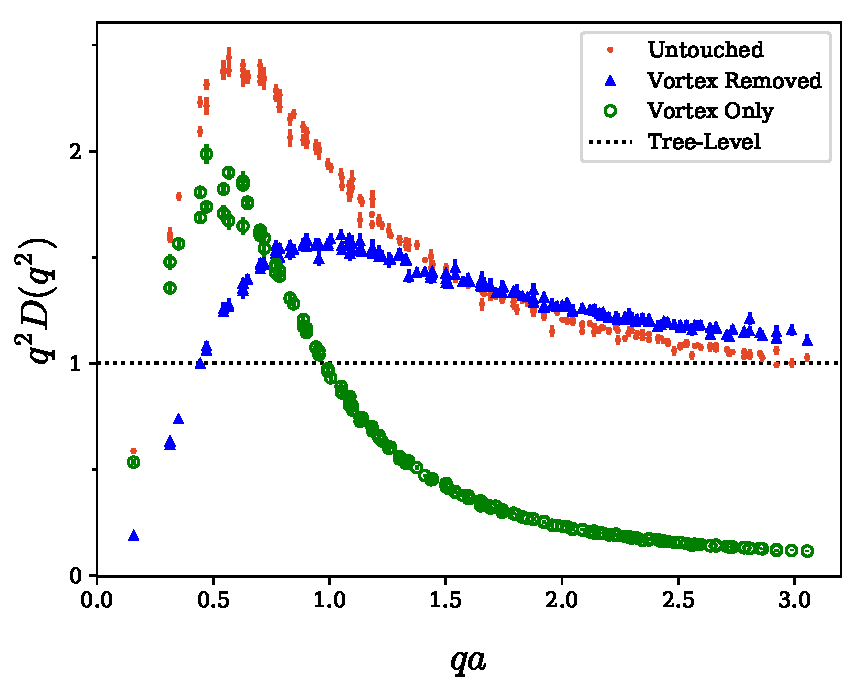
\includegraphics[width=\linewidth]{./ScalarGluComp_q2_NoCoolSum.pdf}
\caption{\label{fig:NoCool}The gluon propagator calculated from the original untouched (red dots), shown with the vortex removed (blue triangles) and vortex only (green open circles) results. Here, the renormalisation factor for the vortex removed and vortex only propagators is chosen to be the same as for the untouched propagator.}
\end{figure}
%
\begin{figure}[tb]
\centering
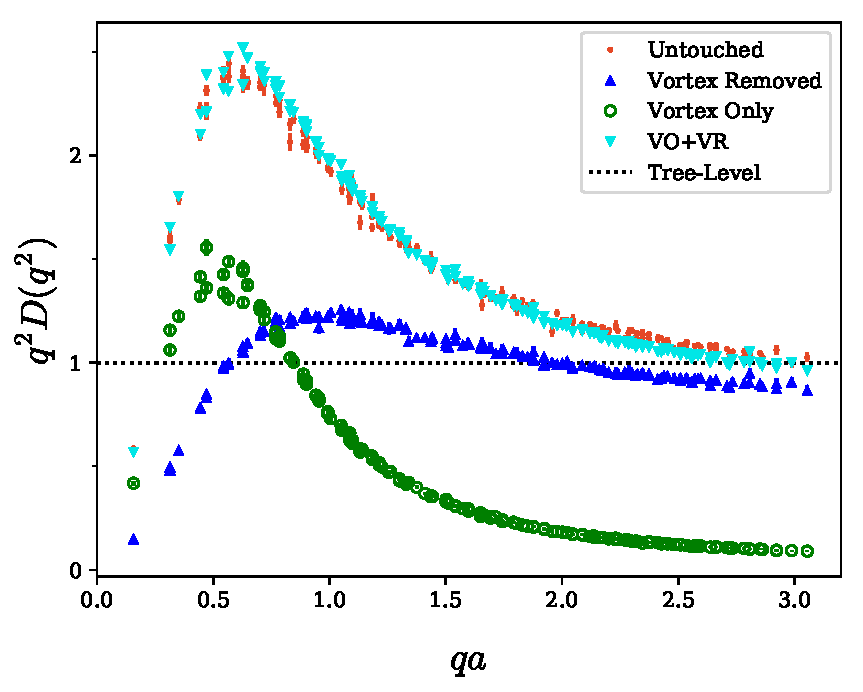
\includegraphics[width=\linewidth]{./ScalarGluComp_q2_NoCoolSum2.pdf}
\caption{\label{fig:NoCoolSum}The gluon propagator from the original untouched ensemble as in Fig.~\ref{fig:NoCool}, now shown with the independently renormalised sum (cyan triangles) of the vortex removed and vortex only propagators. The two vortex modified propagators are also shown, but here their renormalisation factor is chosen to be the same as for the summed propagator.}
\end{figure}

Calculating the scalar propagator on untouched, vortex-removed and vortex only configurations gives the results illustrated in Fig.~\ref{fig:NoCool}. To make contact with the tree-level propagator at large $q^2$, we renormalise such that $q^2D(q^2)=1$ for $qa = 3.0$ on the original configurations, and apply this same renormalisation factor to the vortex removed and vortex only propagators. The vortex removed configurations display the expected behaviour, with vortex removal corresponding to significant infrared suppression of the propagator when compared to the untouched propagator, in agreement with the results of Ref.~\cite{Bowman:2010zr}. The increased roughness of the gauge fields after vortex removal is evidenced by the enhancement of the propagator at large $q$. This reflects the increase in short-distance fluctuations that have been introduced to the gauge fields by the vortex removal procedure.\\

It is interesting to note that the vortex only propagator retains approximately two thirds of the untouched propagator's peak strength. This is comparable to previous work showing partial recovery of the string tension on vortex only configurations~\cite{Trewartha:2015ida,Trewartha:2017ive,Langfeld:2003ev,Stack:2002sy}. Despite only recovering a portion of the original strength, the infrared peak is still considerably greater than the peak observed in the vortex removed propagator. The loss of strength is most likely in part because of the known imperfections in the vortex identification algorithm that results in some vortex matter remaining in the vortex removed configurations. The vortex only configurations also exhibit a loss of short range strength, due to the absence of the high frequency modes that are instead contained within the vortex removed field.\\

If we sum the vortex only and vortex removed propagators and independently renormalise such that $q^2\,D(q^2)=1$ at $qa=3.0$, we obtain the result shown in Fig.~\ref{fig:NoCoolSum}. Here we observe agreement between the untouched and summed propagators. This indicates that vortex modification effectively partitions the lattice configuration into short range physics on the vortex removed configurations and long range physics on the vortex only configurations, up to errors in the vortex identification procedure.

\subsection{Partitioning}

\begin{figure}[tb]
\centering
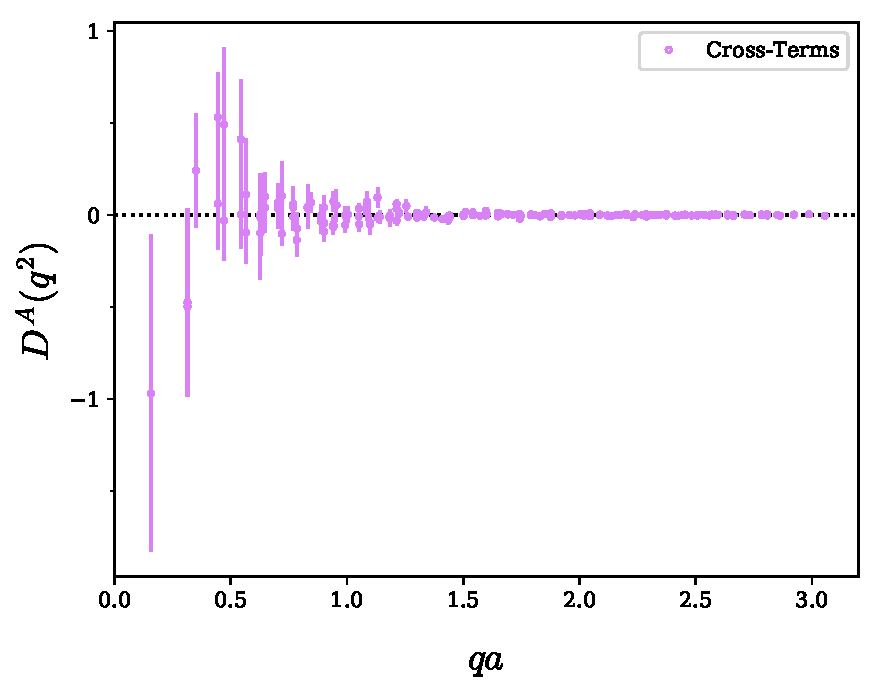
\includegraphics[width=\linewidth]{./ScalarGluComp_q2_CrossTerms.pdf}
\caption{\label{fig:CrossTerms} Calculation of the cross-terms arising from Eq.~\ref{eq:Partition}}
\end{figure}

This partitioning is expected if the vortex removed and vortex only configurations are orthogonal. To see how this behaviour emerges, suppose that we can decompose the gluon field $A_\mu$ into two independent fields as follows
\begin{equation}
  A_\mu(p) = B_\mu(p) + C_\mu(p).
\end{equation}
In the context of this work, we associate $B_\mu$ with the background field of short-range gluon fluctuations and $C_\mu$ with the centre vortex field.
Note also that if $B$ and $C$ are in Landau gauge then so is $A.$ Using this partitioning it follows that the gluon propagator for $A$ can be written as the sum of the respective gluon propagators for $B$ and $C,$
\begin{align}
  D^{A}_{\mu\nu}(p) &= \frac{1}{V}\langle A_\mu(p) \, A_\nu(-p) \rangle\nonumber \\
  &= \frac{1}{V}\Big(\langle B_\mu(p)B_\nu(-p)\rangle + \langle C_\mu(p)C_\nu(-p)\rangle\nonumber\\
   &~~~~~~~+ \langle B_\mu(p)C_\nu(-p)+ C_\mu(p)B_\nu(-p) \rangle\Big)\nonumber \\
  &= D^{B}_{\mu\nu}(p) + D^{C}_{\mu\nu}(p),\label{eq:Partition}
\end{align}
where we have made use of the fact that $B$ and $C$ represent orthogonal degrees of freedom in the gauge field and hence in the ensemble average the cross-correlations should vanish. These cross-correlations are explicitly calculated by evaluating 
\begin{equation}
D_{\text{cross-terms}}(p^2) = \frac { 2 } { 3 \left( n _ { c } ^ { 2 } - 1 \right) V } \left\langle \operatorname { Tr } \left( B_\mu(p)C_\mu(-p)+ C_\mu(p)B_\mu(-p) \right) \right\rangle\, ,
\label{eq:CTprop}
\end{equation}
analogous to the scalar gluon propagator derived in Chapter~\ref{chapter:GluonPropagator}. The results of this calculation are shown in Fig.~\ref{fig:CrossTerms}. As can be clearly seen, in the ensemble average Eq.~\ref{eq:CTprop} vanishes, indicating that the vortex only and vortex removed configurations truly do represent a orthogonal degrees of freedom.\\  

To elucidate the connection to the unitary formulation of the lattice gauge links, we suppose that we can transform $A$ to an ``ideal centre gauge'' such that in lattice units the field $C$ consists purely of centre phases,
\begin{equation}
C_\mu(x) = k\,\frac{2\pi}{3} I,\quad k\in \{-1,0,+1\}.
\end{equation}
On a continuous manifold we can write the Wilson line corresponding to a lattice link as a path-ordered exponential,
\begin{equation}
U_{\mu}(x) = \mathcal{P} e^{i\int_0^1 d\lambda \,A_{\mu}(x+\lambda\hat{\mu})}.
\end{equation}
The lattice midpoint approximation replaces the integral as follows,
\begin{equation}
U_{\mu}(x) = e^{iA_{\mu}(x+\hat{\mu}/2)}.
\end{equation}
As $A = B + C$ it immediately follows that we can write
\begin{equation}
U_{\mu}(x) = e^{i B_{\mu}(x+\hat{\mu}/2)} \, e^{i C_{\mu}(x+\hat{\mu}/2)},
\end{equation}
noting that in our ideal centre gauge $[B,C] = 0$ so the Baker-Campbell-Haussdorff relation is trivial. Identifying
\begin{equation}
Z_{\mu}(x) = e^{i C_{\mu}(x+\hat{\mu}/2)}
\end{equation}
as the vortex-projected field, and
\begin{equation}
R_{\mu}(x) = e^{i B_{\mu}(x+\hat{\mu}/2)}
\end{equation}
as the background remainder field we thus recover the decomposition of the links used herein,
\begin{equation}
U_{\mu}(x) = Z_{\mu}(x)\cdot R_{\mu}(x).
\end{equation}
In practise, on the lattice the maximal centre gauge fixing that is implemented will differ from the ideal centre gauge postulated here due to apparent numerical difficulties in simultaneously identifying all vortex matter within an $SU(3)$ gauge field. What this means is that the projected field $Z$ may not capture all of the vortex matter such that there is some non-trivial topological structures that remain in the background field $R.$ The infrared enhancement in the vortex removed results in Fig.~\ref{fig:NoCool} suggests this is the case.\\

\subsection{Renormalisation}

In Fig.~\ref{fig:NoCoolSum} it proved necessary to independently renormalise the untouched and summed propagators such that they agree at $qa=3.0$. The necessity of this renormalisation is worth discussing, as it is important to motivate why comparison between the original and reconstructed propagators is valid. To do this, it is beneficial to first consider the renormalised gluon propagator in the continuum. The renormalised propagator at any loop order, $D_R^\text{C}(q^2)$ can be related to the bare propagator, $D^\text{C}(q^2)$ via the relationship
%
\begin{equation}
D^\text{C}(q^2) = Z^\text{C}_3 \, D_R^\text{C}(q^2)\, .
\label{eq:ContinuumRenormalisation}
\end{equation}
%
Typically $Z^\text{C}_3$ and $D^\text{C}(q)$ are infinite, whereas $D_R^\text{C}(q)$ is finite. The renormalised propagator is not independent of the renormalisation scheme, and the expression for $Z^\text{C}_3$ depends on the renormalisation scheme employed. For example, in the minimal subtraction (MS) scheme at one-loop order with no quark fields, $Z_3^\text{C}=1+\frac{5g^2}{8\pi^2\epsilon}$~\cite{ryder1996quantum}, where the quantity $\epsilon$ is introduced during the analytic continuation to $d = 4-\epsilon$ dimensions as part of the dimensional regularisation procedure. However, regardless of the chosen renormalisation scheme, the renormalised propagator can always be expressed in the form shown in Eq.~\ref{eq:ContinuumRenormalisation}~\cite{vanRitbergen:1997va}.\\

On the lattice, we can explicitly calculate the now finite bare dimensionless propagator $D^\text{L}(q^2)$, as the lattice introduces an explicit momentum cutoff of $\frac{\pi}{a}$. In the language of the continuum, this can be thought of as an approximation of the continuum bare propagator to all loop orders. Similarly, the lattice renormalisation constant $Z_3(\mu, a)$ is also finite. On the lattice, Eq.~\ref{eq:ContinuumRenormalisation} becomes
%
\begin{equation}
a^2 D^\text{L}(q^2) = Z_3(\mu, a)\, D_R(q^2)\, ,
\label{eq:LatticeRenormalisation}
\end{equation}
%
where the $a^2$ factor restores the dimensionality of the left-hand side of the equation. Despite the finiteness of $D^\text{L}(q^2)$ and $Z_3(\mu, a)$, it is still necessary to enforce a renormalisation scheme to be able to draw meaningful comparisons between propagators. As such, we employ the momentum space subtraction (MOM) scheme~\cite{Bowman:2004jm,Leinweber:1998uu,Bonnet:2001uh}, which requires that for some sufficiently large $\mu$
%
\begin{equation}
D_R(q^2)\big|_{q^2=\mu^2}=\frac{1}{\mu^2}\, .
\end{equation}
%
This sets the value of the renormalisation constant to be
%
\begin{equation}
Z_3(\mu,a) = a^2 \, \mu^2 \, D^\text{L}(\mu^2)\, ,
\end{equation}
such that
%
\begin{equation}
D_R(q^2) = \frac{D^\text{L}(q^2)}{\mu^2 \, D^\text{L}(\mu^2)}\, .
\end{equation}
%
This renormalised propagator is what we plot in e.g. Fig.~\ref{fig:NoCoolSum}. The value of $\mu$ is arbitrary, however it is necessary that it is sufficiently large such that it is outside the infrared region where the gluon propagator exhibits substantial deviation from tree-level behaviour. Furthermore, $\mu$ must be away from the momentum cutoff, as the renormalisation constant is only independent of the cutoff in the limit that the cutoff tends towards infinity~\cite{Bonnet:2001uh,Boucaud:2006pc}. Given the momentum range of $qa\in [0,4.6]$, arising from the momentum variables described in Sec.~\ref{sec:MomentumVariables}, a choice of $\mu =3.0$ satisfies both conditions. Additionally, it also falls below the maximum momentum of $qa = 3.1$ imposed by the momentum half-cut described in Sec.~\ref{sec:LatticeParameters}. Once the renormalisation scheme has been imposed, it is then possible to connect the lattice results with those obtained from perturbation theory by connecting the renormalisation constant with those obtained from the MS or modified minimal subtraction (\textoverline{\text{MS}}) schemes.\\

This discussion of renormalisation has motivated why it is acceptable to compare the untouched and summed propagators in Fig.~\ref{fig:NoCoolSum}; it is the renormalised propagator, not the bare propagator, that carries the physical meaning. Hence, the fact that the untouched and summed propagators agree after renormalisation is an important result indicating the effective partitioning of the gluon propagator under vortex modification. The final point worth discussing is the renormalisation applied to the vortex only and vortex removed propagators. Given that we don't have an {\it a priori} expectation of the tree-level behaviour, imposing the MOM condition lacks meaning. Instead, to facilitate comparisons, we make use of the original $Z_3(\mu, a)$ obtained for the untouched propagator unless specified otherwise. Maintaining this consistency is sufficient to comment on the qualitative shape of the propagator, which is the most significant point of interest in this research. 

%\textcolor{red}{\textbf{Renormalisation steps:}
%\begin{enumerate}
%\item Calculation contains divergent integrals that must be isolated.
%\item Dimensional regularisation isolates the infinities in the integral.
%\item Redefine the mass/coupling to absorb these infinities. The new constant is \textit{finite}, whereas the original constant is taken to be \textit{infinite}.
%\item Alternatively, the counter term method can be used.
%\item The counter term method states that the original constant is \textit{finite}, that are modified by infinite constants.
%\item Upon calculating physical quantities, the infinite constants cancel off the infinities arising from the loop integrals.
%\end{enumerate}
%\textbf{Questions:}
%\begin{enumerate}
%\item At what scale does $D_{\text{QED}}(q^2) = \frac{1}{q^2}$?
%\item At what scale can we suppose that $D_{\text{QED}}(q^2) = D_{\text{QCD}}(q^2)$
%\item Is it reasonable to say that the condition that must be enforced on the combined propagator is $D(q^2) = \frac{1}{q^2}$ at some large momentum, and as such this is the normalisation that should be applied to the VR and VO propagators?
%\item Does $D_{\text{QCD}}(q^2)$ equal the bare continuum propagator at a fixed cutoff?
%\item What does the renormalised propagator correspond to in the continuum? 
%\end{enumerate}
%}

\section{Impact of Cooling}

\begin{figure}[tb]
\centering
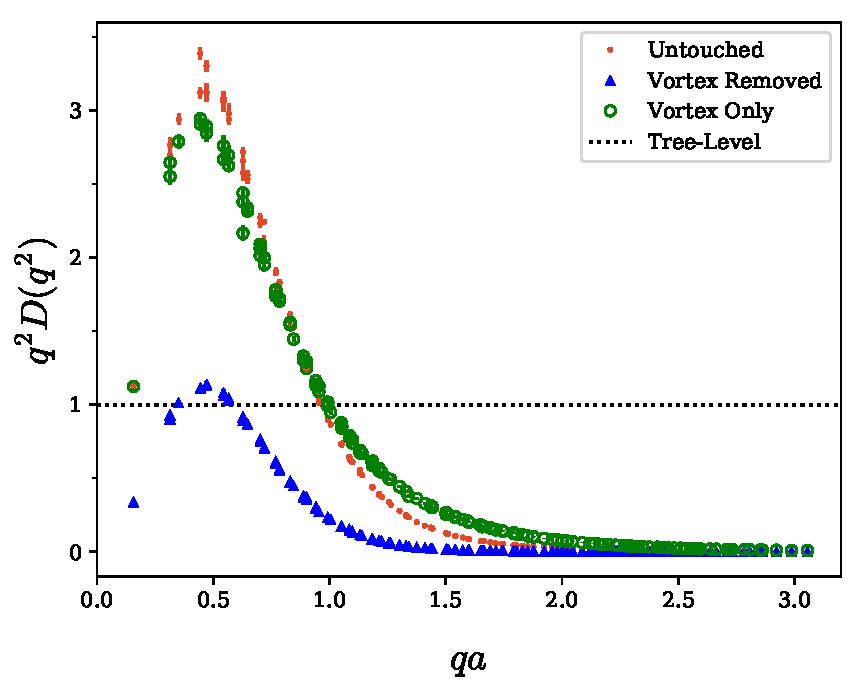
\includegraphics[width=\linewidth]{./ScalarGluComp_q2_10sweepsAll.pdf}
\caption{\label{fig:10SweepsCooling}The gluon propagator calculated on the three ensembles after 10 sweeps of cooling. We now observe an improved agreement between the untouched and vortex only propagators.}
\end{figure}  
%
After performing 10 sweeps of cooling on the untouched, vortex-removed and vortex-only ensembles, we obtain the results shown in Fig.~\ref{fig:10SweepsCooling}. As is typical of cooling, the removal of short range structures means that all three ensembles tend to zero as $q\rightarrow\infty$. There is now a noticeable improvement in the agreement between the untouched and vortex only configurations; however there is still a difference present, especially in the $qa\approx0.5$ and $qa\approx1.5$ regions.\\

We perform the same analysis of the vortex only propagator under cooling as performed in Sec.~\ref{sec:CoolingGluProp} on the untouched propagator. Once again in gauge fixing, each sweep is preconditioned by the Landau gauge transformation of the previous sweep in descending order. The result of this analysis is shown in Fig.~\ref{fig:1to10VO}. This figure shows a similar change in the vortex only propagator when compared to the untouched propagator in Fig.~\ref{fig:1to10SweepsCooling}, with an enhancement in the infrared and suppression in the UV modes. The UV suppression is less noticeable in this case due to the prior removal of short range effects brought about by the vortex identification.\\

%
\begin{figure}[tb]
\centering
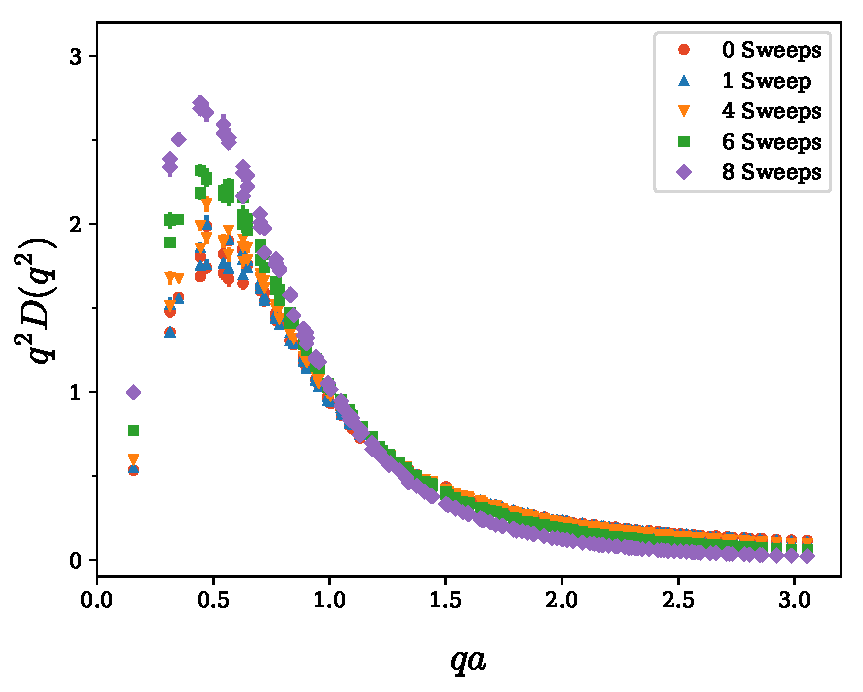
\includegraphics[width=\linewidth]{./ScalarGluComp_q2_1to10sweepsVO.pdf}
\caption{\label{fig:1to10VO}The vortex only propagator after different sweeps of cooling. A trend similar to Fig.~\ref{fig:1to10SweepsCooling} is observed, with enhancement in the infrared and suppression in the UV region.}
\end{figure}
%
We observe that the vortex only and untouched propagators in Fig.~\ref{fig:10SweepsCooling} resemble the gluon propagator under a differing number of sweeps of cooling, as shown in Fig.~\ref{fig:1to10SweepsCooling} and Fig.~\ref{fig:1to10VO}. The vortex only propagator has a peak that sits below the untouched propagator, and the untouched propagator is further suppressed in the $qa\approx 1.5$ region. Following the trend in Fig.~\ref{fig:1to10SweepsCooling} and Fig.~\ref{fig:1to10VO}, this indicates that further cooling on the vortex only propagator would align it with the untouched propagator. This follows from an understanding that the vortex-only configurations are initially much rougher than their untouched counterparts~\cite{Trewartha:2015nna}, and should therefore require additional cooling to obtain agreement with the untouched configurations.\\
%
\begin{figure}[tb]
\centering
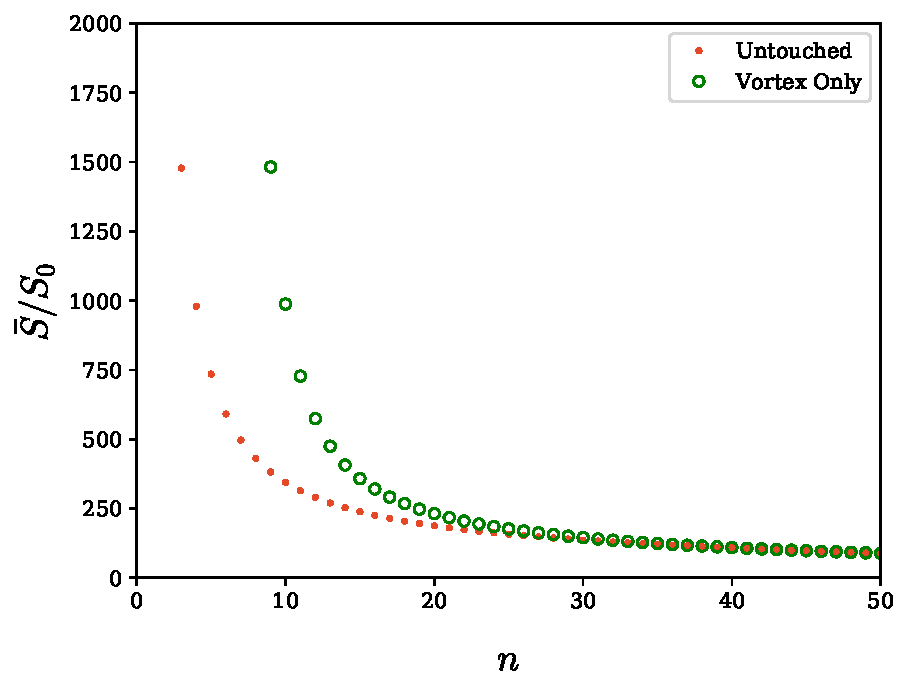
\includegraphics[width=\linewidth]{./ActionMatch.pdf}
\caption{\label{fig:ActionMatch}The average action calculated on the untouched and vortex-only configurations as a function of cooling sweeps, $n$. The vortex only configurations are initially rougher than the untouched, as evidenced by the higher average action.}
\end{figure}
%
\begin{table}[tb]
\caption{\label{tab:ActionMatch}Comparison of the number of cooling sweeps on the untouched ($n_U$) and vortex only ($n_{VO}$) configurations required to match the average action.}
\centering
\begin{tabular}{c | c | c | c}
$n_U$ & $\bar{S}/S_0$ & $n_{VO}$ & $\bar{S}/ S_0$\\
\hline
5 & $734.83$ & 11 & $727.67$\\
10 & $344.22$ & 15 & $357.68$\\
15 & $238.21$ & 20 & $231.19$\\
20 & $187.55$ & 24 & $184.68$\\
25 & $156.92$ & 28 & $155.72$\\
30 & $135.91$ & 32 & $135.61$\\
35 & $120.29$ & 36 & $120.66$\\
40 & $107.08$ & 40 & $109.02$\\
\end{tabular}
\end{table}
%
\begin{figure}[tb]
\centering
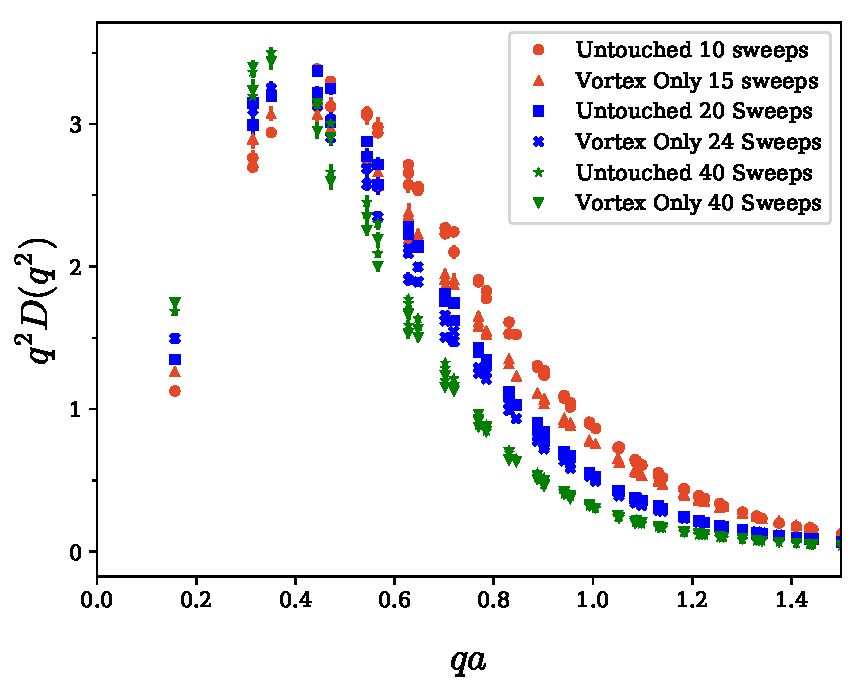
\includegraphics[width=\linewidth]{./ScalarGluComp_q2_UVOActionMatch.pdf}
\caption{\label{fig:UVOActionMatch}Comparison of the gluon propagator on the untouched and vortex only configurations after tuning the number of cooling sweeps to best match the average plaquette action. This procedure gives a much better agreement in the shape of the gluon propagator from the two configurations.}
\end{figure}
%

We take the average $\mathcal{O}(a^4)$ three-loop improved action of the lattice divided by the single instanton action $S_0=\frac{8\pi^2}{g^2}$, denoted $\bar{S}/S_0$, to be a measure of roughness. We observe that for $n<20$ cooling sweeps the vortex-only configurations have a significantly higher action than their untouched counterparts after the same number of sweeps of cooling, as illustrated in Fig.~\ref{fig:ActionMatch}. We therefore seek to find the number of sweeps required to best match the action between the vortex-only and untouched configurations. The results of this procedure are shown in Table \ref{tab:ActionMatch}. If we now plot these matched configurations, we obtain the results shown in Fig.~\ref{fig:UVOActionMatch}. Here we have truncated the plot at large $qa$ to better show the agreement in the mid-$qa$ region. By matching the actions as closely as possible with an integer number of cooling sweeps, we see that there is a better agreement between the untouched and vortex-only gluon propagators.\\

\section{Summary}
The results presented above concur with the now significant body of evidence that centre vortices contain the essential degrees of freedom of the Yang-Mills vacuum, such that the application of smoothing enables the recreation of the major features of QCD~\cite{Bertle:2001xd,Trewartha:2015ida,Trewartha:2015nna,Trewartha:2017ive,DelDebbio:1998luz}. We have shown that vortex identification partitions the gluon propagator into low and high momentum modes, with the vortex only configurations encapsulating the majority of the infrared strength. Cross-correlation between the vortex only and vortex removed propagators can be seen to vanish in the ensemble average. By cooling the configurations, we observe that the vortex only configurations are continuously suppressed, while the infrared peak in the untouched and vortex only propagator acquires better agreement. By tuning the number of cooling sweeps to best match the average action of the vortex only and untouched configurations, we can effectively match the gluon propagators obtained from each of these configurations.\\

%
\begin{figure}
\centering
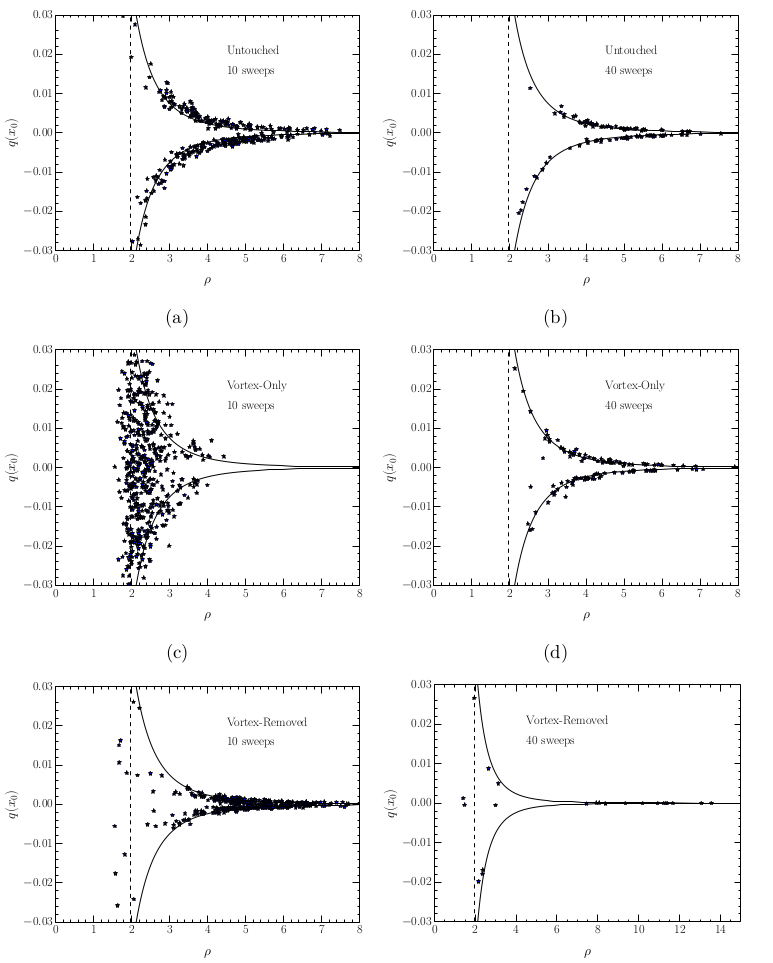
\includegraphics[width=\linewidth]{./Instanton_Radius.png}
\caption{\label{fig:InstantonRadius} The topological charge at the instanton centre, $q(x_0)$, is plotted against the instanton radius $\rho$ for the vortex modified configurations under 10 and 40 sweeps of cooling. The solid line represents the theoretical distribution. These plots are acquired from \citet{Trewartha:2015ida}.}
\end{figure}
%
Noting that sufficient smoothing of a vortex-only field generates a topological background of instanton-like objects, we can regard the thin centre vortices as the seeds of instantons. The smoothing process that is applied on the vortex-only configurations raises a question regarding the precise role of vortices in the restoration of the infrared propagator; is it simply the presence of (sufficiently smoothed) vortices or is it more indirectly the reformation of the instanton background? If we examine Fig.~\ref{fig:10SweepsCooling}, we see that after the application of 10 sweeps of cooling the vortex-only propagator has the appropriate qualitative infrared behaviour. Comparing with previous work, in particular Fig.~7 within Ref.~\cite{Trewartha:2015ida} (replicated in Fig.~\ref{fig:InstantonRadius}) which shows the typical distribution of the instanton radius against the topological charge at the centre, we can see that after only 10 sweeps of cooling the vortex-only distribution still deviates significantly from the ideal theoretical instanton relationship. This suggests that it is the smoothed centre vortices that are directly responsible for the infrared structure of the gluon propagator.
%!TEX root = ../thesis.tex
%*******************************************************************************
%*********************************** Seventh Chapter *****************************
%*******************************************************************************

\chapter{Centre Vortex Visualisations}
\ifpdf
    \graphicspath{{Chapter7/Figs/Raster/}{Chapter7/Figs/PDF/}{Chapter7/Figs/}}
\else
    \graphicspath{{Chapter7/Figs/Vector/}{Chapter7/Figs/}}
\fi

In previous chapters we have motivated the significance of centre vortices in QCD through the calculation of the gluon propagator. Although we can predict many of the properties of vortices through calculation, these properties can also be explored through visualisations of the lattice. To this end, in this chapter we present a novel visualisation technique that allows us to view thin centre vortices on the lattice through the use of three-dimensional (3D) models.

\section{Time Slices}
As the lattice is a four-dimensional hypercube, we visualise the centre vortices on 3D slices. The choice of dimension to take slices along is irrelevant in Euclidean space, so we choose to take slices along the $x$-axis, resulting in $N_x$ slices each with dimension $N_y\times N_z\times N_t$. This choice of axis to slice along allows for the largest volume per slice.  However, the transition between slices is best thought of as `stepping though time', so we re-label our coordinates such that each slice is a snapshot at fixed $t$, with local coordinates $(x,y,z)$. Within each slice we can visualise all vortices associated with an $x-y$, $x-z$ or $y-z$ plaquette by calculating $P_{x\,y}(\bf{x})$, $P_{y,z}(\bf{x})$ and $P_{z,x}(\bf{x})$ for all $\bf{x}$ in the slice. These vortices will be referred to as the `space-oriented' vortices, as they are fixed in time. The plaquettes are evaluated on a centre projected configuration, so $P_{\mu\nu}\in \lbrace -1,\,0,\,+1\rbrace$. For a $+1$ vortex, a blue jet is plotted piercing the centre of the plaquette, and for a $-1$ vortex a red jet is plotted. The direction of the jet is set according to a right-hand rule, such that
\begin{itemize}[leftmargin=*,itemsep=0pt,labelsep=12pt]
\item $P_{x\,y}=\pm 1\implies \pm\hat{z}$ direction.
\item $P_{y\,z}=\pm 1\implies \pm\hat{x}$ direction.
\item $P_{x\,z}=\pm 1\implies \mp\hat{y}$ direction,
\end{itemize}
An example of this plotting convention is shown in Fig.~\ref{fig:SpacialVortices}.\\

\begin{figure}[ht]
\centering
  \begin{subfigure}[b]{0.3\textwidth}
  \centering
  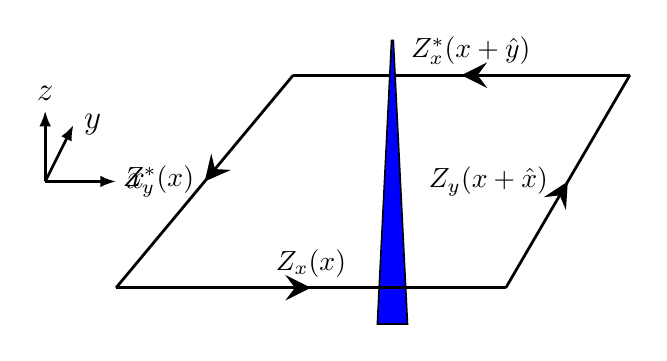
\begin{tikzpicture}[scale=0.9]
\begin{scope}[very thick,decoration={
    markings,
    mark=at position 0.5 with {\arrow[scale=2]{stealth}}}
    ] 
  % bottom right to top right                    x,y start of line    label  x,y end
  \draw[line width=1.0,postaction={decorate}](1.5,-1.5)-- node[left]{$Z_y(x+\hat x)\ $} (3.25,1.5)node(g){};
  % top right to top left
  \draw[line width=1.0,postaction={decorate}](3.25,1.5)-- node[above]{${}\ \ Z_x^*(x+\hat y)$} (-1.5,1.5);
  % top left to bottom left
  \draw[line width=1.0,postaction={decorate}](-1.5,1.5)-- node[left]{$Z_y^*(x)$}(-4,-1.5);

  % Jet triangle
  % bottom left	
  \draw (-0.3,-2) node(a){}
  -- (0.1,-2) node(b){}   % bottom right
  -- (-0.1,2) node(c){}   % top
  -- cycle;               % complete
  \fill[blue] (a.center) -- (b.center) -- (c.center);
  
  % bottom left to bottom right
  \draw[line width=1.0,postaction={decorate}](-4,-1.5)-- node[above]{$Z_x(x)$}(1.5,-1.5)node(f){};
  
  \draw[line width=1.0,-{Latex[length=2mm]}](-5,0)--(-4,0.0)node[right]{\large $x$};
  \draw[line width=1.0,-{Latex[length=2mm]}](-5,0)--(-4.6,0.8)node[right]{\large $y$};
  \draw[line width=1.0,-{Latex[length=2mm]}](-5,0)--(-5,1.0)node[above]{\large $z$};
  \end{scope}
  
\end{tikzpicture}
  \end{subfigure}
  \hfill
  \begin{subfigure}[b]{0.55\textwidth}
  \centering
  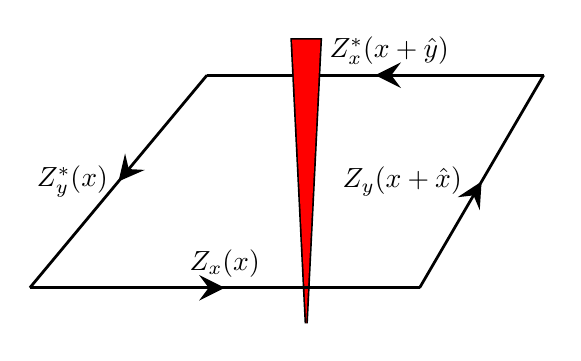
\begin{tikzpicture}[scale=0.9]
\begin{scope}[very thick,decoration={
    markings,
    mark=at position 0.5 with {\arrow[scale=2]{stealth}}}
    ] 
  % bottom right to top right                    x,y start of line    label  x,y end
  \draw[line width=1.0,postaction={decorate}](1.5,-1.5)-- node[left]{$Z_y(x+\hat x)\ $} (3.25,1.5)node(g){};
  % top right to top left
  \draw[line width=1.0,postaction={decorate}](3.25,1.5)-- node[above]{\quad $Z_x^*(x+\hat y)$} (-1.5,1.5);
  % top left to bottom left
  \draw[line width=1.0,postaction={decorate}](-1.5,1.5)-- node[left]{$Z_y^*(x)$}(-4,-1.5);

  % Jet triangle
  \draw (-0.3,2) node(a){}
  -- (0.1,2) node(b){}
  -- (-0.1,-2)node(c){}
  -- cycle;
  \fill[red] (a.center) -- (b.center) -- (c.center);
  
  % bottom left to bottom right
  \draw[line width=1.0,postaction={decorate}](-4,-1.5)-- node[above]{$Z_x(x)$}(1.5,-1.5)node(f){};
  
  % Coordinate axes       arrow head          x,y start -- x,y finish [position] label
  \end{scope}
\end{tikzpicture}
  \end{subfigure}             
  \caption{An example of the plotting convention for vortices located within a 3D time slice. \textbf{Left:} A $+1$ vortex in the $+\hat{z}$ direction. \textbf{Right:} A $-1$ vortex in the $-\hat{z}$ direction.}
  \label{fig:SpacialVortices}
\end{figure}
%
The 3D slices for $t=1,2$ with the space-oriented vortices plotted appear as in Figs.~\ref{fig:PlaqT01}, \ref{fig:PlaqT02}. At first glance the vortex structure appears highly complex, and it is difficult to identify the significant features. As such, we make use of the 3D models to hone in and isolate the important features present in these slices. We present some of these features in Fig.~\ref{fig:VortexFeatures}.\\

%
{\centering
\begin{figure}[htb!]
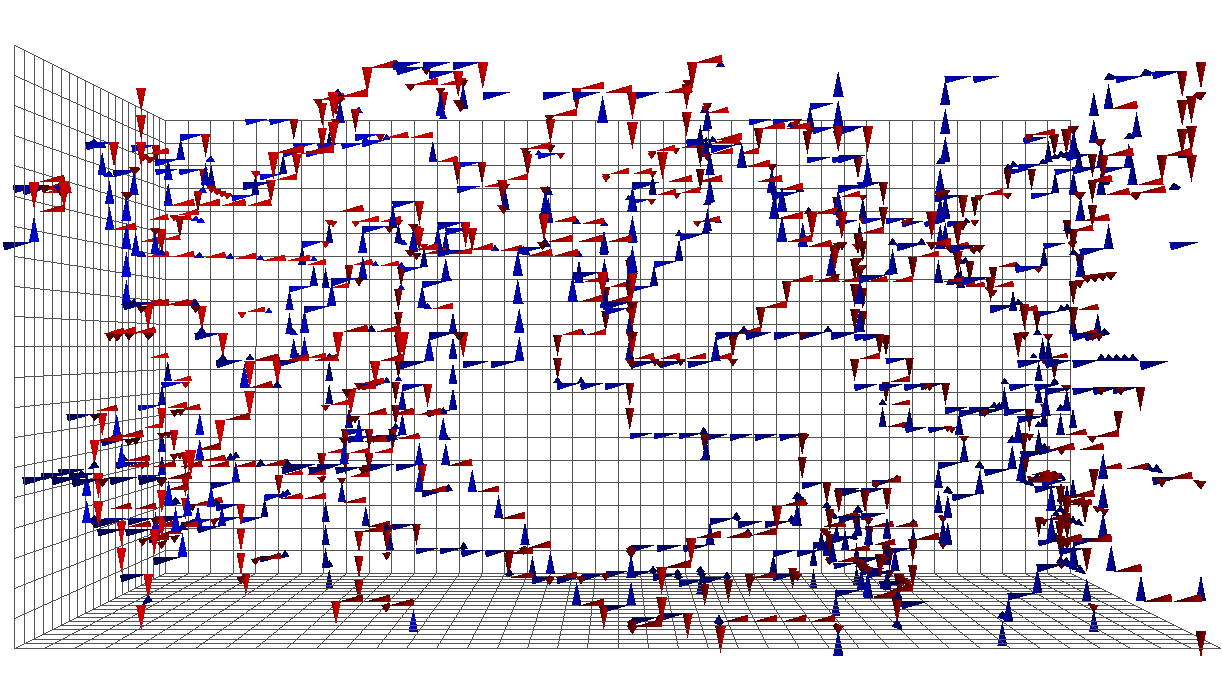
\includegraphics[width=\linewidth]{Plaq_CFG95_T01.png}
\caption{\label{fig:PlaqT01}The $t=1$ slice with all space-oriented vortices plotted.}
\end{figure}
}
%
{\centering
\begin{figure}[htb!]
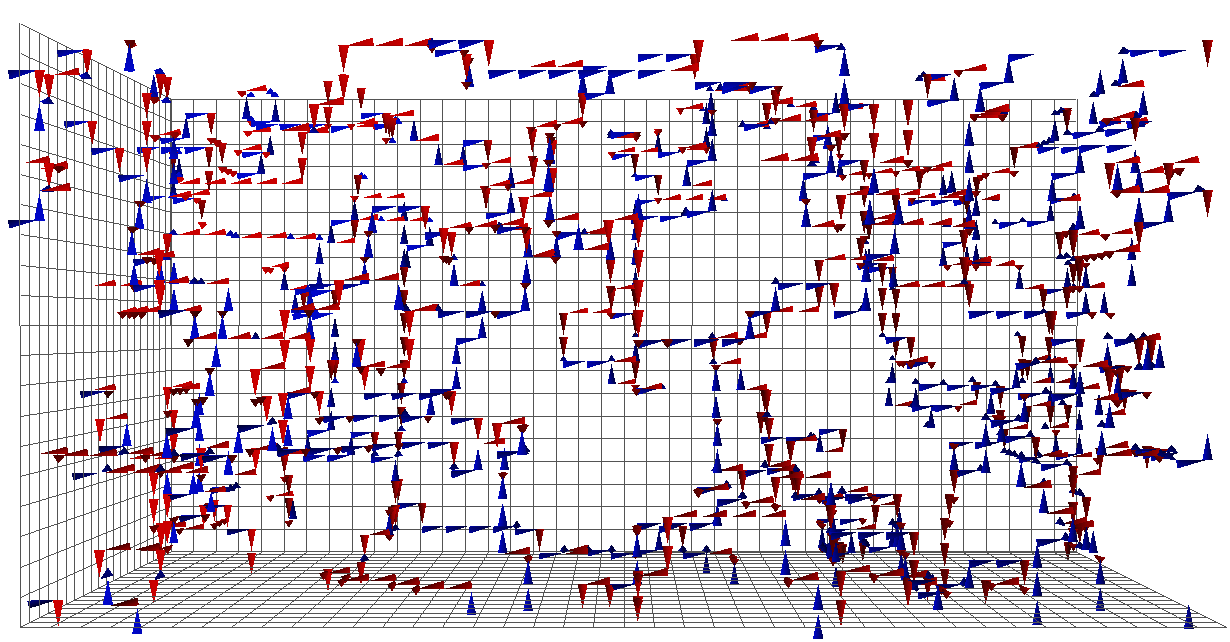
\includegraphics[width=\linewidth]{Plaq_CFG95_T02.png}
\caption{\label{fig:PlaqT02}The $t=2$ slice with all space-oriented vortices plotted.}
\end{figure}
}
%
\begin{figure}[htb!]
\centering
    \begin{subfigure}[b]{0.3\textwidth}
	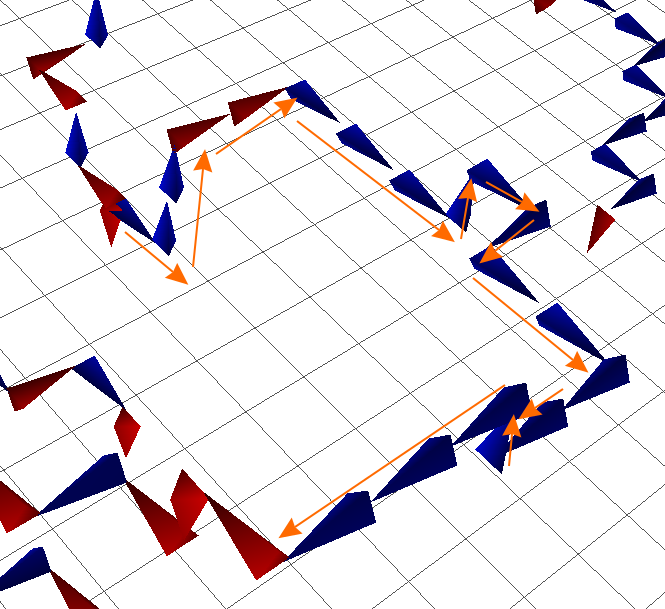
\includegraphics[width=\textwidth]{./plaqt1_line.png}
    \end{subfigure}\hfill
    \begin{subfigure}[b]{0.3\textwidth}
    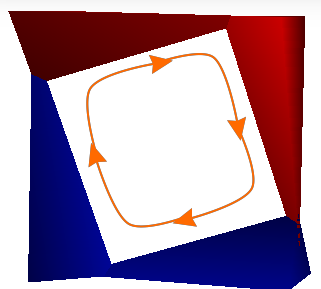
\includegraphics[width=\textwidth]{./plaqt1_loop.png}
    \end{subfigure}\hfill
    \begin{subfigure}[b]{0.3\textwidth}
	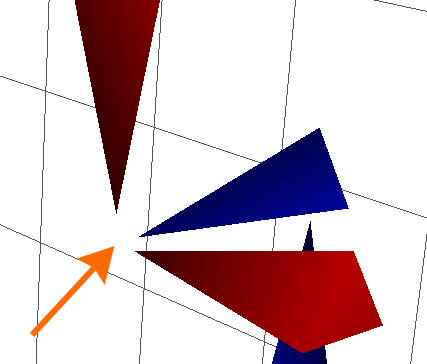
\includegraphics[width=\textwidth]{./plaqt1_monopole.png}
    \end{subfigure}
    \caption{\label{fig:VortexFeatures} \textbf{Left:} Vortices form continuous lines. Note that because of the lattice periodicity, these lines may wrap around to the opposite edge of the lattice. \textbf{Middle:} Vortices must form closed loops to conserve the vortex flux. \textbf{Right:} $SU(3)$ vortices are capable of forming monopoles or branching points where three vortices emerge or converge at a single point.}
\end{figure}
%
It is an excellent sanity check to see that the vortices do indeed form closed lines, as they must to conserve the centre flux and satisfy the Bianchi identity~\cite{Engelhardt:2003wm,Spengler:2018dxt}. We also observe that with the exception of the $1\times 1$ vortex loops (see the middle image in Fig.~\ref{fig:VortexFeatures}) which can be readily attributed to incorrectly identified centre phases, the vortex loops are large and do not form isolated loops within the 3D volume. This agrees with the observation made of $SU(2)$ vortices in Ref.~\cite{Engelhardt:1999fd} that below the critical deconfinement temperature, $T_C$, almost all vortices identified had the maximum possible extent. It will be the subject of future work to investigate whether as the temperature increases the $SU(3)$ vortices begin to shrink and cease to percolate, indicating a transition to the deconfining phase.\\

The presence of branching/monopole points is of particular interest, as previous studies have primarily focussed on $SU(2)$ theory which is free from these structures. This is because it is only in $SU(3)$ (or more generally, $SU(N)$ with $N>2$) that it is possible to conserve the centre flux at the intersection of 3 vortices, as shown in Fig.~\ref{fig:VortexBranching}. It is clear from our visualisations that these points occur frequently in the confining phase, in agreement with the findings of Ref.~\cite{Spengler:2018dxt}. The ambiguity between monopoles and branching points arises from the lack of definite orientation for the vortex line. As $P_{\mu\nu} = P_{\nu\mu}^\dagger$, the ordering by which the plaquette is calculated will invert the sign of the vortex, and as such the choice of ordering can change a monopole into a branching point, or vice-versa. The significance of this ambiguity is unclear, but it is worth emphasising its existence. The presence of these points may also be related to the non-vanishing total topological charge observed in the vacuum, and enforces an integer topological charge when they are considered to be `nexus' solutions, as described in Refs.~\cite{Cornwall:1999xw,Cornwall:1998ef}.
%
\begin{figure}[htb!]
\centering
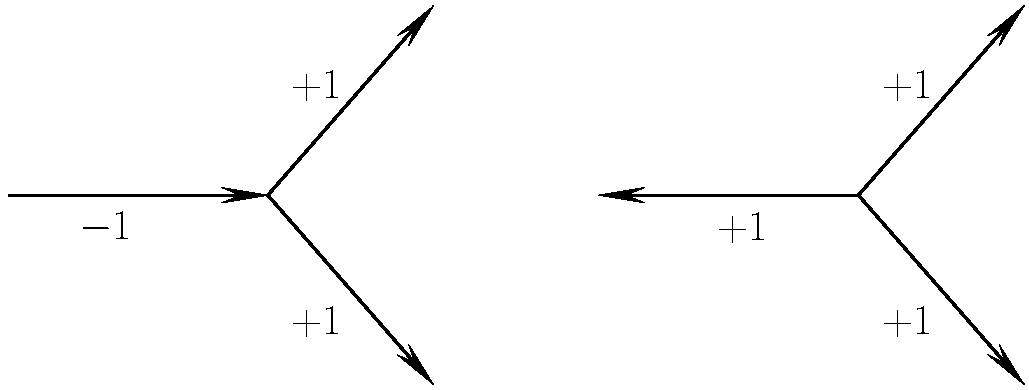
\includegraphics[width=\linewidth]{./VortexBranching.pdf}
\caption{\label{fig:VortexBranching}\textbf{Left:} A vortex branching point. \textbf{Right:} A vortex monopole. Note that for both figures, the vortex charge is conserved at the vertex. By changing the orientation of the plaquette containing the left-most vortex, these two diagrams can be interchanged.}
\end{figure}
%
\section{Time-Oriented vortices}
For each link in a given 3D slice there are two additional plaquettes that lie in the $x_i - t$ plane, pointing in the positive and negative time directions. Vortices associated with time-oriented plaquettes contain information of how the line-like vortices evolve with time, or equivalently, how the vortex surfaces appear in four dimensions. In a given 3D slice we only have access to one link associated with a time-oriented vortex, and as such we plot an arrow along this link to indicate its association with this vortex. We adopt the following plotting convention for these time-oriented vortices:
\begin{itemize}[leftmargin=*,itemsep=0pt,labelsep=12pt]
\item  \makebox[13em][l]{$+1$ vortex, forward in time}  $\implies$ cyan arrow, positively oriented.
\item  \makebox[13em][l]{$+1$ vortex, backward in time} $\implies$ cyan arrow, negatively oriented.
\item  \makebox[13em][l]{$-1$ vortex, forward in time}  $\implies$ orange arrow, positively oriented.
\item  \makebox[13em][l]{$-1$ vortex, backward in time} $\implies$ orange arrow, negatively oriented.
\end{itemize}
An example of these conventions is shown in Fig.~\ref{fig:TimeVortices}. Utilising these conventions, we see that the first two time slices now appear as Figs.~[\ref{fig:PlaqLinkT01}, \ref{fig:PlaqLinkT02}]\\
%
\begin{figure}[ht]
\centering
  \begin{subfigure}[b]{0.45\textwidth}
  \centering
  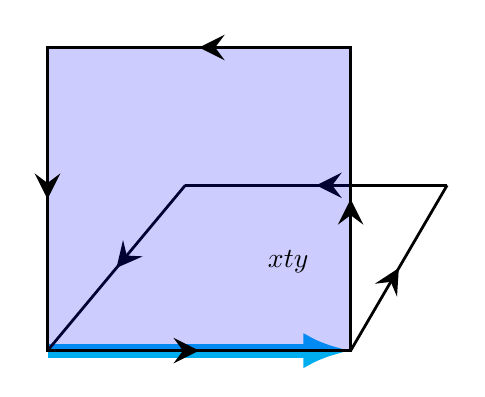
\begin{tikzpicture}[scale=0.7]
% Axes
\tkzDefPoint(-6,-1.5){ax}
\tkzDefShiftPoint[ax](1,0){axR}
\tkzDefShiftPoint[ax](0,1){axT}
\tkzDefShiftPoint[ax](0.6,0.8){axB}

\begin{scope}[very thick,decoration={
    markings,
    mark=at position 0.5 with {\arrow[scale=2]{stealth}}}
    ] 

  % cyan line first to make it look transparent
  \draw[line width=5,color=cyan,-{Latex[length=6mm]}](-4.0,-1.5)--(1.5,-1.5);

  % bottom right to top right                    x,y start of line    label  x,y end
  \draw[line width=1.0,postaction={decorate}](1.5,-1.5)--node[right]{} (3.25,1.5)node(g){};
  % top right to top left
  \draw[line width=1.0,postaction={decorate}](3.25,1.5)--node[above]{} (-1.5,1.5);
  % top left to bottom left
  \draw[line width=1.0,postaction={decorate}](-1.5,1.5)--node[left]{} (-4,-1.5);

  \filldraw[fill=blue,fill opacity=0.2] (-4,-1.5) -- (1.5,-1.5) -- (1.5,4) -- (-4,4)--cycle;

  %% % Jet triangle
  %% % bottom left	
  %% \draw (-0.3,-2) node(a){}
  %% -- (0.1,-2) node(b){}   % bottom right
  %% -- (-0.1,2) node(c){}   % top
  %% -- cycle;               % complete
  %% \fill[red] (a.center) -- (b.center) -- (c.center);
  
  % bottom left to bottom right
  \draw[line width=1.0,postaction={decorate}](-4.0,-1.5)--node[above]{}(1.5,-1.5)node(f){};
  
  % t direction  
  \draw[line width=1.0,postaction={decorate}]( 1.5,-1.5)--node[right]{} (1.5,4.0);    % width  3.25-(-1.5) = 4.75
  \draw[line width=1.0,postaction={decorate}]( 1.5, 4.0)--node[above]{}(-4.0,4.0);    % height 6.25-1.5    = 4.75
  \draw[line width=1.0,postaction={decorate}](-4.0, 4.0)--node[left]{}(-4.0,-1.5);

  \end{scope}
  
% Draw Axes
\tkzDrawSegments[thick,->, >=stealth](ax,axR)
\tkzDrawSegments[thick,->, >=stealth](ax,axT)
\tkzDrawSegments[thick,->, >=stealth](ax,axB)
\tkzLabelPoint[right](axR){$x$}
\tkzLabelPoint[above](axT){$t$}
\tkzLabelPoint[above](axB){$y$}
\end{tikzpicture}
  \end{subfigure}
  \hfill
  \begin{subfigure}[b]{0.45\textwidth}
  \centering
  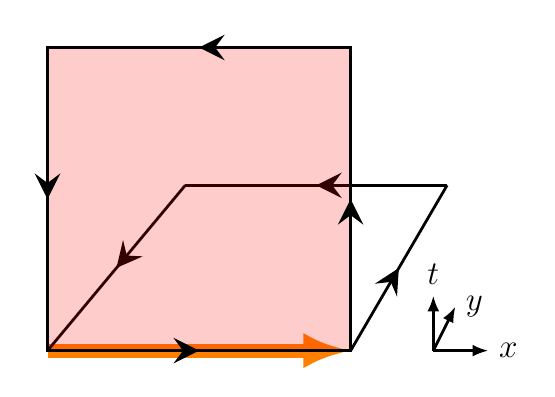
\begin{tikzpicture}[scale=0.7]
\begin{scope}[very thick,decoration={
    markings,
    mark=at position 0.5 with {\arrow[scale=2]{stealth}}}
    ] 

  % orange line first to make it look transparent
  \draw[line width=5,color=orange,-{Latex[length=6mm]}](-4.0,-1.5)--(1.5,-1.5);

  % bottom right to top right                    x,y start of line    label  x,y end
  \draw[line width=1.0,postaction={decorate}](1.5,-1.5)--node[right]{} (3.25,1.5)node(g){};
  % top right to top left
  \draw[line width=1.0,postaction={decorate}](3.25,1.5)--node[above]{} (-1.5,1.5);
  % top left to bottom left
  \draw[line width=1.0,postaction={decorate}](-1.5,1.5)--node[left]{} (-4,-1.5);

    \filldraw[fill=red,fill opacity=0.2] (-4,-1.5) -- (1.5,-1.5) -- (1.5,4) -- (-4,4)--cycle;
  
  %% % Jet triangle
  %% % bottom left	
  %% \draw (-0.3,-2) node(a){}
  %% -- (0.1,-2) node(b){}   % bottom right
  %% -- (-0.1,2) node(c){}   % top
  %% -- cycle;               % complete
  %% \fill[red] (a.center) -- (b.center) -- (c.center);
  
  % bottom left to bottom right
  \draw[line width=1.0,postaction={decorate}](-4.0,-1.5)--node[above]{}(1.5,-1.5)node(f){};
  
  % t direction  
  \draw[line width=1.0,postaction={decorate}]( 1.5,-1.5)--node[right]{} (1.5,4.0);    % width  3.25-(-1.5) = 4.75
  \draw[line width=1.0,postaction={decorate}]( 1.5, 4.0)--node[above]{}(-4.0,4.0);    % height 6.25-1.5    = 4.75
  \draw[line width=1.0,postaction={decorate}](-4.0, 4.0)--node[left]{}(-4.0,-1.5);

  % Coordinate axes       arrow head          x,y start -- x,y finish [position] label
  \draw[line width=1.0,-{Latex[length=2mm]}](3,-1.5)--(4,-1.5)node[right]{\large $x$};
  \draw[line width=1.0,-{Latex[length=2mm]}](3,-1.5)--(3.4,-0.7)node[right]{\large $y$};
  \draw[line width=1.0,-{Latex[length=2mm]}](3,-1.5)--(3,-0.5)node[above]{\large $t$};
  \end{scope}
\end{tikzpicture}
  \end{subfigure}             
  \caption{\textbf{Left:} A $+1$ vortex in the forward $x-t$ plane (shaded blue) will be plotted as a cyan arrow in the $+\hat{x}$ direction. \textbf{Right:} A $-1$ vortex in the forward $x-t$ plane (shaded red) will be plotted as an orange arrow in the $+\hat{x}$ direction.}
  \label{fig:TimeVortices}
\end{figure}
%
\begin{figure}[htb!]
\centering
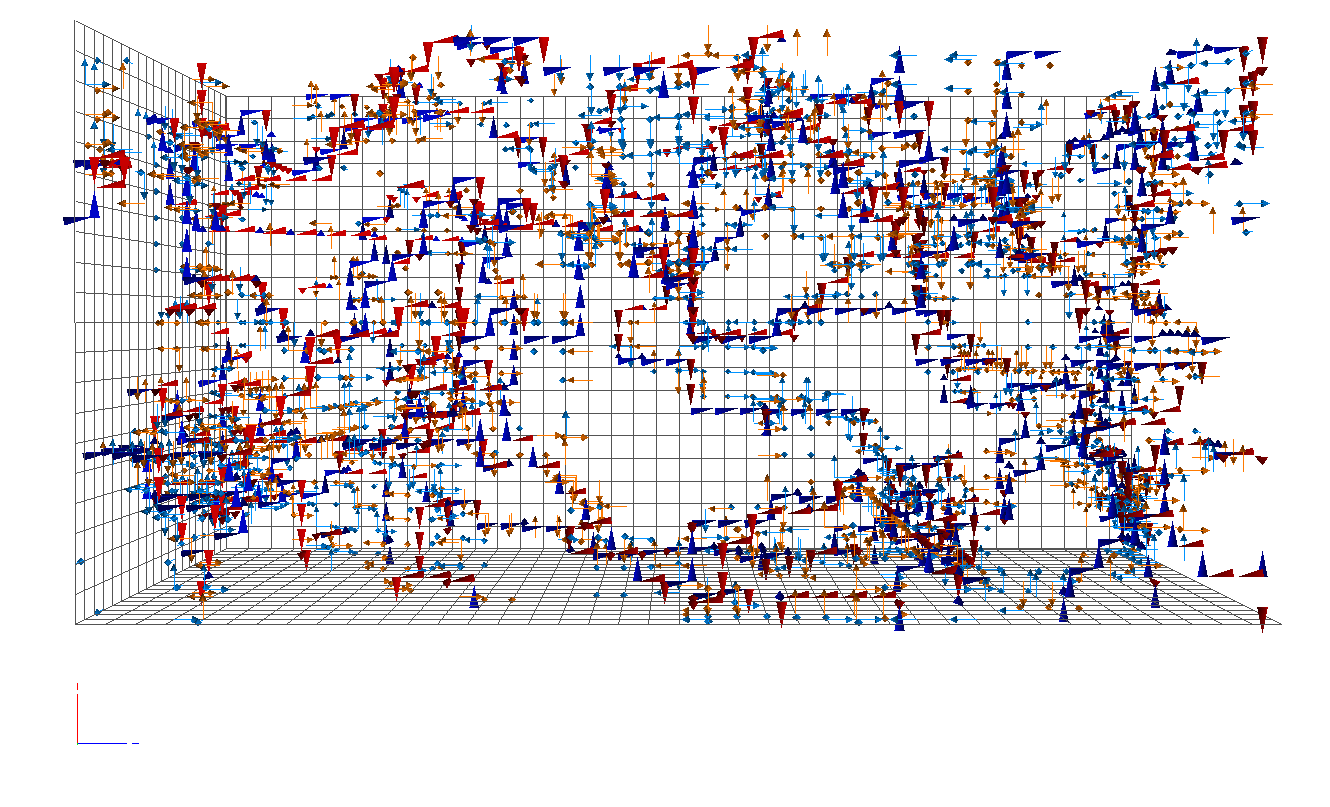
\includegraphics[width=\linewidth]{PlaqLink_CFG95_T01.png}
\caption{\label{fig:PlaqLinkT01}The $t=1$ slice with all space-oriented and time-oriented vortices plotted.}
\end{figure}
%
\begin{figure}[htb!]
\centering
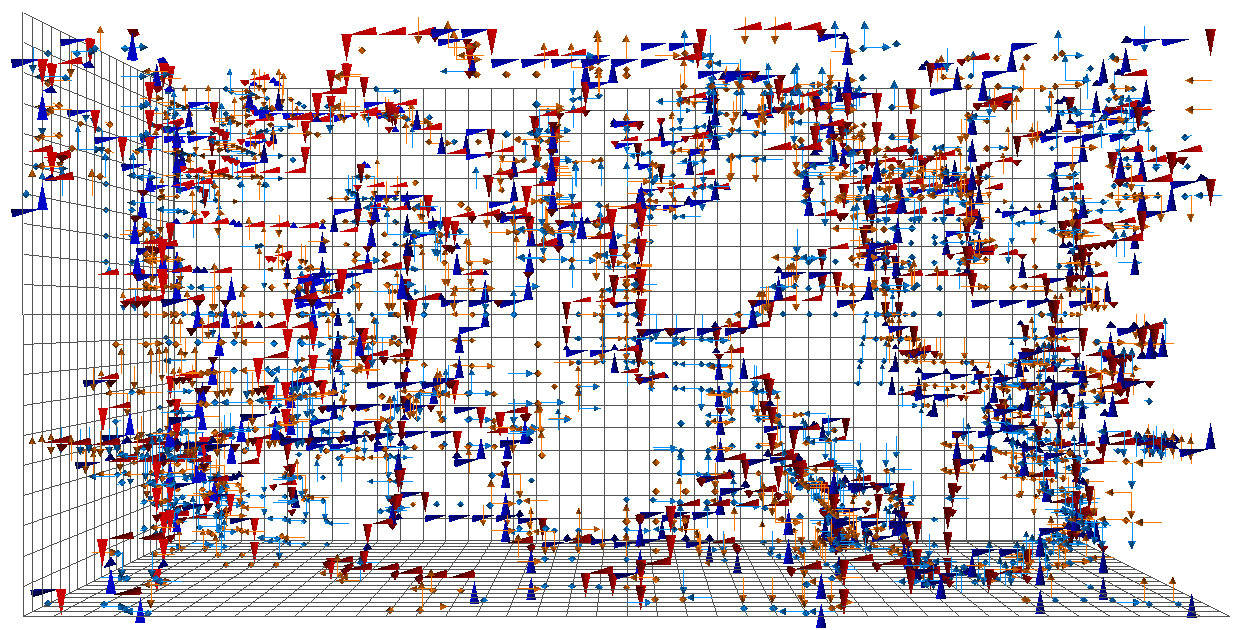
\includegraphics[width=\linewidth]{PlaqLink_CFG95_T02.png}
\caption{\label{fig:PlaqLinkT02}The $t=2$ slice with all space-oriented and time-oriented vortices plotted.}
\end{figure}
%

As we step through time, we expect to see the positively oriented vortices swap direction as they transition from being forwards in time to backwards in time, as shown in Fig.~\ref{fig:VortexArrows}. The time-oriented vortices act as predictors of vortex motion between slices. To see this, consider Fig.~\ref{fig:VortexMotion}. In Fig.~\ref{fig:VortexMotion1}, we observe a line of four $-1$ (red) vortices with no time-oriented links associated with them, indicating that this line should remain fixed as we step through time. Alternatively, towards the top of the red line we observe a branching point with two associated $-1$ time-oriented arrows, indicating that this branching point should move in the direction of the time-oriented vortices. Observing the same region at $t=2$ in Fig.~\ref{fig:VortexMotion2}, we see that this is precisely what occurs. The vortex line has remained fixed, whereas the branching point has shifted one lattice spacing to the left, in accordance with the direction indicated by the time-oriented vortex.\\
%
\begin{figure}[htb!]
\centering
\begin{subfigure}[b]{0.45\textwidth}
\centering
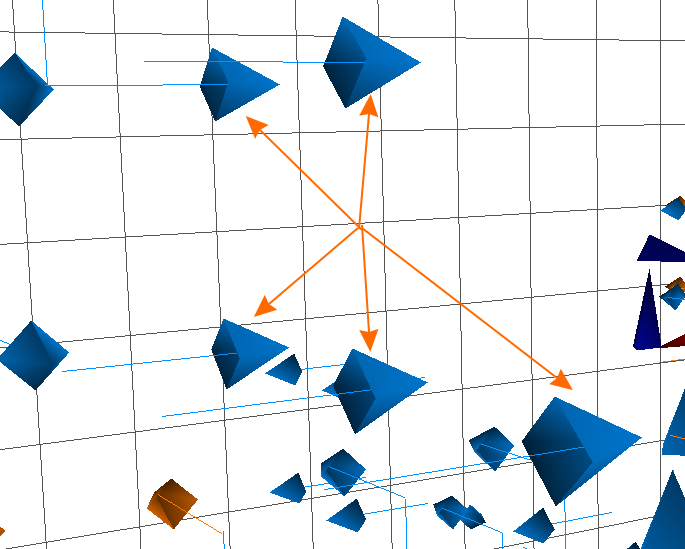
\includegraphics[height=0.2\textheight]{./plaqlinet1_forwardarrows.png}
\subcaption{\label{fig:VortexArrows1}$t=1$}
\end{subfigure}
\hfill
\begin{subfigure}[b]{0.45\textwidth}
\centering
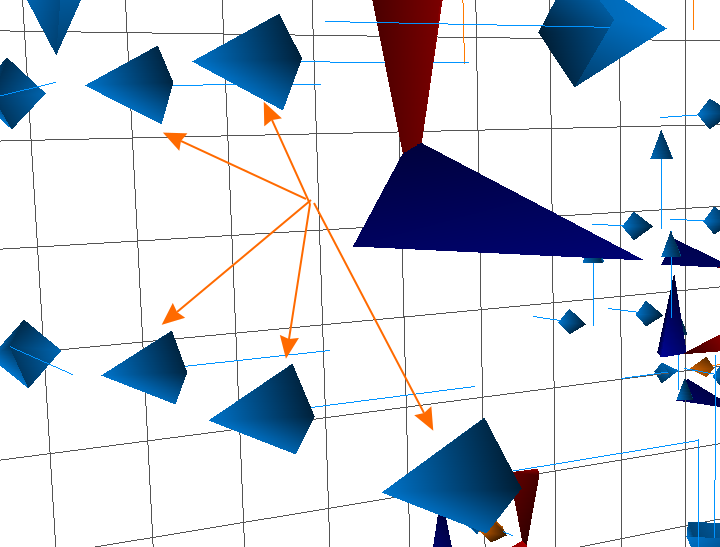
\includegraphics[height=0.2\textheight]{./plaqlinet2_backwardarrows.png}
\caption{\label{fig:VortexArrows2}$t=2$}
\end{subfigure}
\caption{\label{fig:VortexArrows}As we step through time we observe the time-oriented arrows change direction, however the phase (colour) of the vortex remains the same.}
\end{figure}
%
\begin{figure}[htb!]
\centering
\begin{subfigure}[b]{0.45\textwidth}
\centering
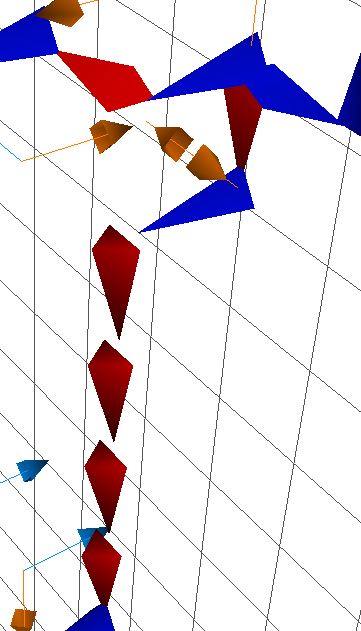
\includegraphics[height=0.4\textheight]{./plaqlinet1_line&monopole.png}
\subcaption{\label{fig:VortexMotion1}$t=1$}
\end{subfigure}
\hfill
\begin{subfigure}[b]{0.45\textwidth}
\centering
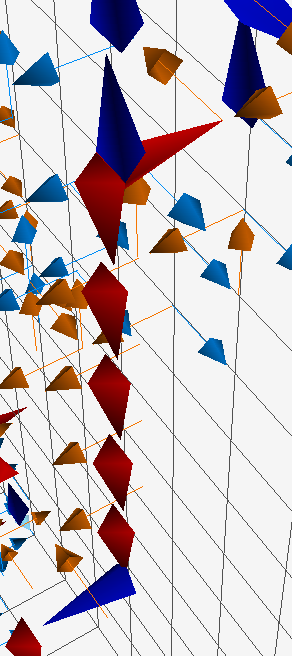
\includegraphics[height=0.4\textheight]{./plaqlinet2_line&monopole.png}
\caption{\label{fig:VortexMotion2}$t=2$}
\end{subfigure}
\caption{\label{fig:VortexMotion}An example of time-oriented vortices predicting the motion of the space-oriented vortices.}
\end{figure}
%

Another example of time-oriented vortices predicting the motion of vortices is shown in Fig.~\ref{fig:VortexLineMotion}. Here we see in Fig.~\ref{fig:VortexLineMotion1} a line of three $+1$ space-oriented vortices each with an associated $-1$ time-oriented vortex below them. As we step to $t=2$ in Fig.~\ref{fig:VortexLineMotion2} we observe the time-oriented arrows change direction as expected, and the space-oriented vortex line shifts one lattice spacing down such that the time-oriented vortices are now above them.\\
\begin{figure}[htb!]
\centering
\begin{subfigure}[b]{0.45\textwidth}
\centering
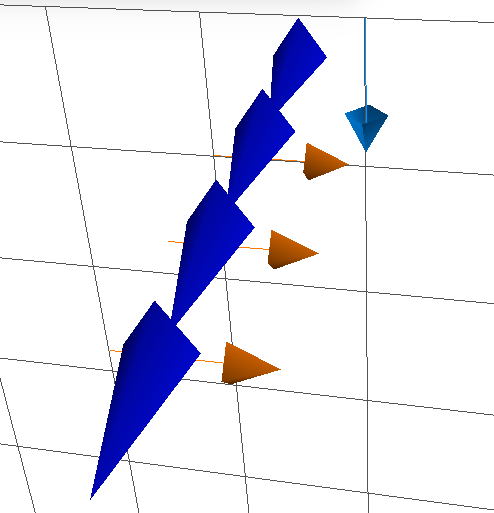
\includegraphics[height=0.3\textheight]{./plaqlinet1_SW8_line.png}
\subcaption{\label{fig:VortexLineMotion1}$t=1$}
\end{subfigure}
\hfill
\begin{subfigure}[b]{0.45\textwidth}
\centering
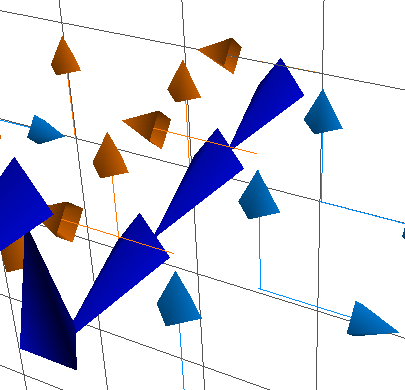
\includegraphics[height=0.3\textheight]{./plaqlinet2_SW8_line.png}
\caption{\label{fig:VortexLineMotion2}$t=2$}
\end{subfigure}
\caption{\label{fig:VortexLineMotion}A second example of time-oriented vortices predicting the motion of the space-oriented vortices. Here we see the $+1$ (blue) vortex line transition one lattice spacing down as we step from $t=1$ to $t=2$.}
\end{figure}
%

The cases presented in Fig.~\ref{fig:VortexMotion} and Fig.~\ref{fig:VortexLineMotion} are ideal, where the space-oriented vortex shifts only one lattice spacing between time slices. However, it is frequently the case where the space-oriented vortices shift multiple lattice spacings per time step. To see how this occurs diagrammatically, consider Fig.~\ref{fig:ComplexStructure}. The shaded red plaquettes indicate the location of a space-oriented vortex which would be plotted in the suppressed $\hat{x}$ direction. The red line demonstrates how the vortex line pierces between the two time slices. Within each slice we would observe the time-oriented links shown, however the space-oriented vortex appears to move three plaquettes in one time step. These multiple transitions make it harder to track the motion of vortices between time slices; nevertheless, the time-oriented vortices are a useful tool for understanding how centre vortices evolve with time. It is worth making clear that if a space-oriented vortex has no associated time-oriented vortices then it is guaranteed to remain stationary. In this respect, the lack of time-oriented vortices is a clear and valuable indicator of vortex behaviour.
%
\begin{figure}[htb!]
\centering
\def\angThe{30}
\def\angPhi{0}

\tdplotsetmaincoords{\angThe}{\angPhi}
\scalebox{0.6}{\begin{tikzpicture}[tdplot_main_coords]

% Axes
\tkzDefPoint(-5,2){ax}
\tkzDefShiftPoint[ax](2,0){axR}
\tkzDefShiftPoint[ax](0,2){axT}
\tkzDefShiftPoint[ax](1.2,1.6){axB}

\begin{scope}[very thick,decoration={
    markings,
    mark=at position 0.5 with {\arrow[scale=2]{stealth}}}
    ] 
% Vortex line part 1
	\draw[line width=2,color=red,postaction={decorate}] (-3.6, -2.15) -- (-0.25,0);
	
% Bottom left red plaquette 
	\path[fill=red,opacity=0.3] (1,-1.5)--(3.5,1.5)--(-1.5,1.5)--(-4,-1.5)--cycle;
	\draw[line width=6,color=orange,-{Latex[length=6mm]}](1,-1.5)--(3.5,1.5);	
	
	\draw[line width=0.75,postaction={decorate}] (1,-1.5)-- node{} (3.5,1.5)node(g){};
	\draw[line width=0.75,postaction={decorate}](3.5,1.5)-- node{} (-1.5,1.5);
		
	\draw[pattern=north west lines, pattern color=orange](3.5,6.5) -- (1,3.5) -- (1,-1.5) -- (3.5,1.5) -- cycle;
	
	% Vortex line part 2
	\draw[line width=2,color=red,postaction={decorate}] (-0.25,0) -- (12.25,8);	
	
	\draw[line width=0.75,postaction={decorate}](-1.5,1.5)--node{}(-4,-1.5);  
	\draw[line width=0.75,postaction={decorate}] (-4,-1.5) --node{}(1,-1.5)node(f){};

% Top left empty plaquette
	\draw[line width=0.75](-1.5,1.5) -- (1,4.5);
	\draw[line width=0.75](1,4.5) -- (6,4.5);
	\draw[line width=0.75](3.5,1.5) -- (6,4.5);
	
% Bottom of dotted cubes
	\draw[line width=6,color=orange,-{Latex[length=6mm]}](8.5,1.5) -- (11,4.5);
	\draw[line width=6,color=cyan,-{Latex[length=6mm]}](3.5,1.5) -- (8.5,1.5);
	\draw[line width=0.75,dashed] (1,-1.5) -- (6,-1.5);
	\draw[line width=0.75,dashed] (3.5,1.5) -- (8.5,1.5);
	\draw[line width=0.75,dashed] (6,4.5) -- (11,4.5);
	
	\draw[line width=0.75,dashed] (6,-1.5) -- (8.5,1.5);
	\draw[line width=0.75,dashed] (8.5,1.5) -- (11,4.5);
	
% Left side of dotted cubes
	\draw[line width=6,color=orange,-{Latex[length=6mm]}](3.5,6.5) -- (1,3.5);
	
	\draw[line width=0.75,dashed] (1,-1.5) -- (1,3.5);
	\draw[line width=0.75,dashed] (3.5,1.5) -- (3.5,6.5);
	\draw[line width=0.75,dashed] (6,4.5) -- (6,9.5);
	
	\draw[line width=0.75,dashed] (1,3.5) -- (3.5,6.5);
	\draw[line width=0.75,dashed] (3.5,6.5) -- (6,9.5);
	
% Top of dotted cubes
	\draw[line width=6,color=orange,-{Latex[length=6mm]}](11,9.5) -- (8.5,6.5);	
	\draw[line width=6,color=cyan,-{Latex[length=6mm]}](8.5,6.5) -- (3.5,6.5);
	\draw[pattern=north west lines, pattern color=cyan] (8.5,6.5) -- (3.5,6.5) -- (3.5,1.5) -- (8.5,1.5) -- cycle;
	
	\draw[line width=0.75,dashed] (1,3.5) -- (6,3.5);
	\draw[line width=0.75,dashed] (3.5,6.5) -- (8.5,6.5);
	\draw[line width=0.75,dashed] (6,9.5) -- (11,9.5);
	
	\draw[line width=0.75,dashed] (6,3.5)-- (8.5,6.5);
	\draw[line width=0.75,dashed] (8.5,6.5) -- (11,9.5);
	
% Right side of dotted cubes
	\draw[pattern=north west lines, pattern color=orange] (11,9.5) -- (8.5,6.5) --  (8.5,1.5) -- (11,4.5) -- cycle;
	
	\draw[line width=0.75,dashed] (6,3.5) -- (6,-1.5);
	\draw[line width=0.75,dashed] (8.5,6.5) -- (8.5,1.5);
	\draw[line width=0.75,dashed] (11,9.5) -- (11,4.5);
	
% Bottom right empty plaquette
	\draw[line width=0.75] (6,3.5) -- (11,3.5);
	\draw[line width=0.75] (11,3.5) -- (13.5,6.5);
	
% Top right red plaquette
	\path[fill=red,opacity=0.3] (8.5,6.5)--(13.5,6.5)--(16,9.5)--(11,9.5)--cycle;
	\draw[line width=0.75,postaction={decorate}] (8.5,6.5) -- (13.5,6.5);
	\draw[line width=0.75,postaction={decorate}] (13.5,6.5) -- (16,9.5);
	\draw[line width=0.75,postaction={decorate}] (16,9.5) -- (11,9.5);
	
% Vortex line part 3
	\draw[line width=2,color=red,postaction={decorate}] (12.25,8) -- (15.6,10.15);

% t labels
	\draw[line width=1,loosely dotted] (6,-1.5) -- (14,-1.5)node[right]{$\resizebox{1.5cm}{!}{t=1}$};
	\draw[line width=1,loosely dotted] (11,3.5) -- (14,3.5)node[right]{$\resizebox{1.5cm}{!}{t=2}$};
	
% Draw Axes
\tkzDrawSegments[thick,->, >=stealth](ax,axR)
\tkzDrawSegments[thick,->, >=stealth](ax,axT)
\tkzDrawSegments[thick,->, >=stealth](ax,axB)
\tkzLabelPoint[right](axR){$\resizebox{0.3cm}{!}{y}$}
\tkzLabelPoint[above](axT){$\resizebox{0.3cm}{!}{t}$}
\tkzLabelPoint[above](axB){$\resizebox{0.3cm}{!}{z}$}
  \end{scope}
\end{tikzpicture}}

\caption{\label{fig:ComplexStructure}A demonstration of how space-oriented vortices can transition multiple lattice spacings in a single time step.}
\end{figure}

\section{Topological Charge}\label{sec:TopChargeVis}

%!TEX root = ../thesis.tex
%*******************************************************************************
%*********************************** Eighth Chapter *****************************
%*******************************************************************************

\chapter{Conclusion}

\ifpdf
    \graphicspath{{Chapter8/Figs/Raster/}{Chapter8/Figs/PDF/}{Chapter8/Figs/}}
\else
    \graphicspath{{Chapter8/Figs/Vector/}{Chapter8/Figs/}}
\fi




% ********************************** Back Matter *******************************
% Backmatter should be commented out, if you are using appendices after References
%\backmatter

% ********************************** Bibliography ******************************
\begin{spacing}{0.9}

% To use the conventional natbib style referencing
% Bibliography style previews: http://nodonn.tipido.net/bibstyle.php
% Reference styles: http://sites.stat.psu.edu/~surajit/present/bib.htm

\bibliographystyle{apalike}
%\bibliographystyle{unsrt} % Use for unsorted references  
%\bibliographystyle{plainnat} % use this to have URLs listed in References
\cleardoublepage
\bibliography{References/references} % Path to your References.bib file


% If you would like to use BibLaTeX for your references, pass `custombib' as
% an option in the document class. The location of 'reference.bib' should be
% specified in the preamble.tex file in the custombib section.
% Comment out the lines related to natbib above and uncomment the following line.

%\printbibliography[heading=bibintoc, title={References}]


\end{spacing}

% ********************************** Appendices ********************************

\begin{appendices} % Using appendices environment for more functunality

%%!TEX root = ../thesis.tex
% ******************************* Thesis Appendix A ****************************
\chapter{How to install \LaTeX} 

\section*{Windows OS}

\subsection*{TeXLive package - full version}
\begin{enumerate}
\item	Download the TeXLive ISO (2.2GB) from\\
\href{https://www.tug.org/texlive/}{https://www.tug.org/texlive/}
\item	Download WinCDEmu (if you don't have a virtual drive) from \\
\href{http://wincdemu.sysprogs.org/download/}
{http://wincdemu.sysprogs.org/download/}
\item	To install Windows CD Emulator follow the instructions at\\
\href{http://wincdemu.sysprogs.org/tutorials/install/}
{http://wincdemu.sysprogs.org/tutorials/install/}
\item	Right click the iso and mount it using the WinCDEmu as shown in \\
\href{http://wincdemu.sysprogs.org/tutorials/mount/}{
http://wincdemu.sysprogs.org/tutorials/mount/}
\item	Open your virtual drive and run setup.pl
\end{enumerate}

or

\subsection*{Basic MikTeX - \TeX~ distribution}
\begin{enumerate}
\item	Download Basic-MiK\TeX (32bit or 64bit) from\\
\href{http://miktex.org/download}{http://miktex.org/download}
\item	Run the installer 
\item	To add a new package go to Start >> All Programs >> MikTex >> Maintenance (Admin) and choose Package Manager
\item	Select or search for packages to install
\end{enumerate}

\subsection*{TexStudio - \TeX~ editor}
\begin{enumerate}
\item	Download TexStudio from\\
\href{http://texstudio.sourceforge.net/\#downloads}
{http://texstudio.sourceforge.net/\#downloads} 
\item	Run the installer
\end{enumerate}

\section*{Mac OS X}
\subsection*{MacTeX - \TeX~ distribution}
\begin{enumerate}
\item	Download the file from\\
\href{https://www.tug.org/mactex/}{https://www.tug.org/mactex/}
\item	Extract and double click to run the installer. It does the entire configuration, sit back and relax.
\end{enumerate}

\subsection*{TexStudio - \TeX~ editor}
\begin{enumerate}
\item	Download TexStudio from\\
\href{http://texstudio.sourceforge.net/\#downloads}
{http://texstudio.sourceforge.net/\#downloads} 
\item	Extract and Start
\end{enumerate}


\section*{Unix/Linux}
\subsection*{TeXLive - \TeX~ distribution}
\subsubsection*{Getting the distribution:}
\begin{enumerate}
\item	TexLive can be downloaded from\\
\href{http://www.tug.org/texlive/acquire-netinstall.html}
{http://www.tug.org/texlive/acquire-netinstall.html}.
\item	TexLive is provided by most operating system you can use (rpm,apt-get or yum) to get TexLive distributions
\end{enumerate}

\subsubsection*{Installation}
\begin{enumerate}
\item	Mount the ISO file in the mnt directory
\begin{verbatim}
mount -t iso9660 -o ro,loop,noauto /your/texlive####.iso /mnt
\end{verbatim}

\item	Install wget on your OS (use rpm, apt-get or yum install)
\item	Run the installer script install-tl.
\begin{verbatim}
	cd /your/download/directory
	./install-tl
\end{verbatim}
\item	Enter command `i' for installation

\item	Post-Installation configuration:\\
\href{http://www.tug.org/texlive/doc/texlive-en/texlive-en.html\#x1-320003.4.1}
{http://www.tug.org/texlive/doc/texlive-en/texlive-en.html\#x1-320003.4.1} 
\item	Set the path for the directory of TexLive binaries in your .bashrc file
\end{enumerate}

\subsubsection*{For 32bit OS}
For Bourne-compatible shells such as bash, and using Intel x86 GNU/Linux and a default directory setup as an example, the file to edit might be \begin{verbatim}
edit $~/.bashrc file and add following lines
PATH=/usr/local/texlive/2011/bin/i386-linux:$PATH; 
export PATH 
MANPATH=/usr/local/texlive/2011/texmf/doc/man:$MANPATH;
export MANPATH 
INFOPATH=/usr/local/texlive/2011/texmf/doc/info:$INFOPATH;
export INFOPATH
\end{verbatim}
\subsubsection*{For 64bit OS}
\begin{verbatim}
edit $~/.bashrc file and add following lines
PATH=/usr/local/texlive/2011/bin/x86_64-linux:$PATH;
export PATH 
MANPATH=/usr/local/texlive/2011/texmf/doc/man:$MANPATH;
export MANPATH 
INFOPATH=/usr/local/texlive/2011/texmf/doc/info:$INFOPATH;
export INFOPATH

\end{verbatim}



%\subsection{Installing directly using Linux packages} 
\subsubsection*{Fedora/RedHat/CentOS:}
\begin{verbatim} 
sudo yum install texlive 
sudo yum install psutils 
\end{verbatim}


\subsubsection*{SUSE:}
\begin{verbatim}
sudo zypper install texlive
\end{verbatim}


\subsubsection*{Debian/Ubuntu:}
\begin{verbatim} 
sudo apt-get install texlive texlive-latex-extra 
sudo apt-get install psutils
\end{verbatim}

%%!TEX root = ../thesis.tex
% ******************************* Thesis Appendix B ********************************

\chapter{Installing the CUED class file}

\LaTeX.cls files can be accessed system-wide when they are placed in the
<texmf>/tex/latex directory, where <texmf> is the root directory of the user’s \TeX installation. On systems that have a local texmf tree (<texmflocal>), which
may be named ``texmf-local'' or ``localtexmf'', it may be advisable to install packages in <texmflocal>, rather than <texmf> as the contents of the former, unlike that of the latter, are preserved after the \LaTeX system is reinstalled and/or upgraded.

It is recommended that the user create a subdirectory <texmf>/tex/latex/CUED for all CUED related \LaTeX class and package files. On some \LaTeX systems, the directory look-up tables will need to be refreshed after making additions or deletions to the system files. For \TeX Live systems this is accomplished via executing ``texhash'' as root. MIK\TeX users can run ``initexmf -u'' to accomplish the same thing.

Users not willing or able to install the files system-wide can install them in their personal directories, but will then have to provide the path (full or relative) in addition to the filename when referring to them in \LaTeX.

\end{appendices}

% *************************************** Index ********************************
\printthesisindex % If index is present

\end{document}
